


\newcommand\scaleSLIJICF{0.15}


\subsection{Spray structures}

Once the global sprays have been studied, the discretization process described in $\S$\ref{subsec:SLI_spatial_discretization} can be applied to obtain spatially discretized sprays that conform the SLI for dispersed-phase simulations. The resulting SLIs are from Figures \ref{fig:injectors_sli_uG75_dx10_x05} to \ref{fig:injectors_sli_uG100_dx20_x10_NT}. All sprays have been discretized with grids composed of square probes, hence the convergence-driven discretization process is not applied (it will be done in Chapter \ref{ch6:jicf_lgs_simulations} to illustrate the differences between the convergence-driven and ad-hoc injectors), since the objective here is to describe the spray states for the different sampled sprays. Each probe contains then a spray represented by the characteristics from Table \ref{tab:ch4_sli_injection_parameters_master_slide}: the magnitudes shown in the figures are the SMD, volume flux $q_l$, convergence map and mean velocities in axial, lateral and vertical directions ($u, v, w$ respectively). All magnitudes except for the convergence maps have been interpolated in the grid to generate the contour maps displayed in order to ease visual interpretation of the spray, while the convergence grids are shown through pixel maps. The discretizing grids in each case are shown in the volume-flux map and convergence maps.

Qualitatively, all maps show similar structures in terms of SMD, flux and velocities. The SMD distributions show low values at the bottom of the planes (droplets generated mainly through the surface breakup phenomenon) and higher values at the top part, which are attributed to the ligaments and large droplets emanating from the dense core due to column breakup. A decrease in SMD in the top part of the spray is observed, which is attributed to small droplets being shed from the column ligaments, as it can be observed in the jet view of Figures \ref{fig:JICF_establishment_UG100_lateral} and \ref{fig:JICF_establishment_UG75_lateral}. The liquid volume flux maps $q_l$ exhibit circular patterns where the maximum flux location is located at the spray center around the symmetry plane $y = 0$ and decreases radially outwards towards the spray boundaries. These fluxes maps represent the same magnitude as the fluxes obtained from the IBs and shown in Figure \ref{fig:ibs_spatial_distributions}: the structures are similar both qualitatively and quantitatively when comparing among cases each lagrangian sampling plane with its homonym IB plane, indicating the suitability of the lagrangian tracking algorithm for obtaining spray characteritics from the resolved simulations. The main differences among lagrangian sampling planes and IBs are found when filming is present, which seemps to be captured by the former but not by the latter as shown in the flux maps. The mean axial velocity maps $\overline{u}$ exhibit low velocities at the central, bottom part of the spray plume and larger velocities at the sides. The former region of low axial velocity is the area affected by the wake generated by the dense core, causing droplet's deceleration, while the higher velocities at the sides are attributed to acceleration by the crossflow of the small droplets generated  by surface breakup, since they have a lower relaxation time than big droplets located at the top part. The lateral velocity $\overline{v}$ shows in all cases a symmetric behaviour with respect to the axis $y = 0$ where positive velocities are found for $y > 0$ and negative ones for $y < 0$, reflecting the spray opening along the lateral direction. Regarding the vertical velocities $\overline{w}$, these ones show a layered structure where the magnitude increases from the bottom (sometimes negative values are found, which correspond to the droplets that later will impinge the bottom wall and film) to the top of the spray, indicating that the sprays increases its penetration along the axial direction (as reflected by the trajectories analyzed in $\S$\ref{subsec:ch5_jet_trajectories_results}). The spray boundaries increase along the lateral and vertical directions with increasing axial distance, which is coherent with the shape of the velocity maps in those directions. All these structures are characteristic of liquid JICFs and have been similarly observed in several experimental studies \citemColor[wu_spray_1998,becker_breakup_2002].

The convergence maps for all cases show that local converged sprays are obtained at the probes located around the maximum fuel flux location. The convergence criterion, which was introduced in $\S$\ref{subsec:SLI_spray_convergence}, only considers the droplets size distributions and does not take into account other magnitudes such as velocities: the areas with large fluxes contain more droplets, hence their distributions are closer to convergence than the probes at the spray edges which in some cases might contain only even one or two droplets (and hence are not converged). Furthermore, some cases (such as the spray at x = 15 mm in case UG100\_DX20, Figure \ref{fig:injectors_sli_uG100_dx20_x15}) show converged sprays in the probes that are close to the wall, where filming is present. Their equivalent fluxes maps show that these are higher than the fluxes obtained in the same regions through the interior boundaries methodology (Figure \ref{fig:ibs_spatial_distributions}) or even at the edges of the bottom region: it is believed that these higher local fluxes (which create converged sprays) are created by filming droplets, since the lagrangian tracking projects each liquid structures considering it to be a point particle without mass while in reality the filming liquid entities are complex, deformed structures which displace along the wall (hence viscosity becomes important) and which are not properly represented through the point-particle assumption. Such structures would be sampled twice with the lagrangian tracking algorithm, since they would be projected through the plane at several time instants while in reality they do not move as fast due to their slower displacement along the wall, and hence they would also make the local spray probes to converge faster. The point particle assumptiong was not done with the IBs methodology, which consider only the actual liquid presence at each time instant in the plane, which explains why some filming regions present large fluxes when obtained through the lagrangian sampling methodology but not with the IBs one. A last important observation is the effect of resolution on the convergence maps: for both operating points, the fine resolution maps show more converged probes (i.e. a more converged local spray) than the coarse resolution ones even though the accumulation times sampled are lower (see Table \ref{tab:jicf_SLI_t_prime_accumulation}). This is due to the fact that the fine resolutions resolved better the breakup phenomena and generate more droplets which are better resolved: converged distributions are obtained faster with fine resolutions due to the larger amount of droplets per timestep sampled (despite a lower total amount of droplets sampled in the whole simulation, as Table \ref{tab:jicf_SLI_Ndr_accumulated} shows). 


\subsubsection*{Case UG75\_DX10}



%%%%%%%%%%%%%%%% UG75_DX10, x = 5 mm


\begin{figure}[h!]
\centering
\begin{subfigure}[b]{0.3\textwidth}
	\centering
   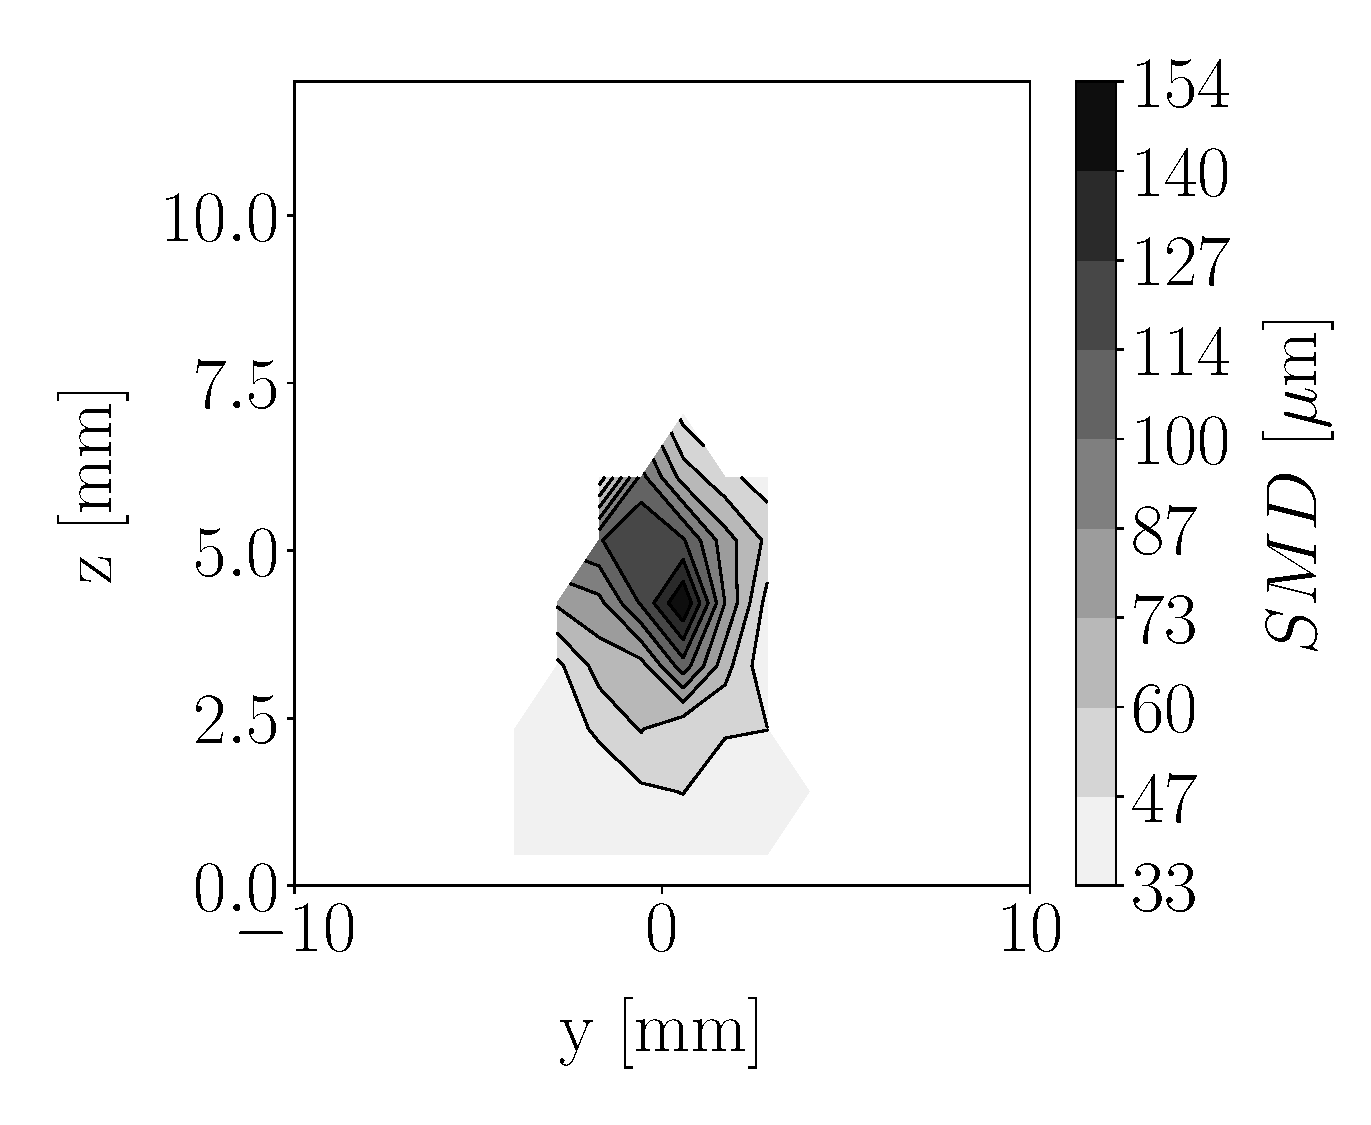
\includegraphics[scale=\scaleSLIJICF]{./part2_developments/figures_ch5_resolved_JICF/injectors_SLI/uG75_dx10_x05_SMD_map}
   %\caption{Case UG100\_DX20: crossflow planes}
   %\label{} 
\end{subfigure}
   \hspace{0.17in}
\begin{subfigure}[b]{0.3\textwidth}
	\centering
   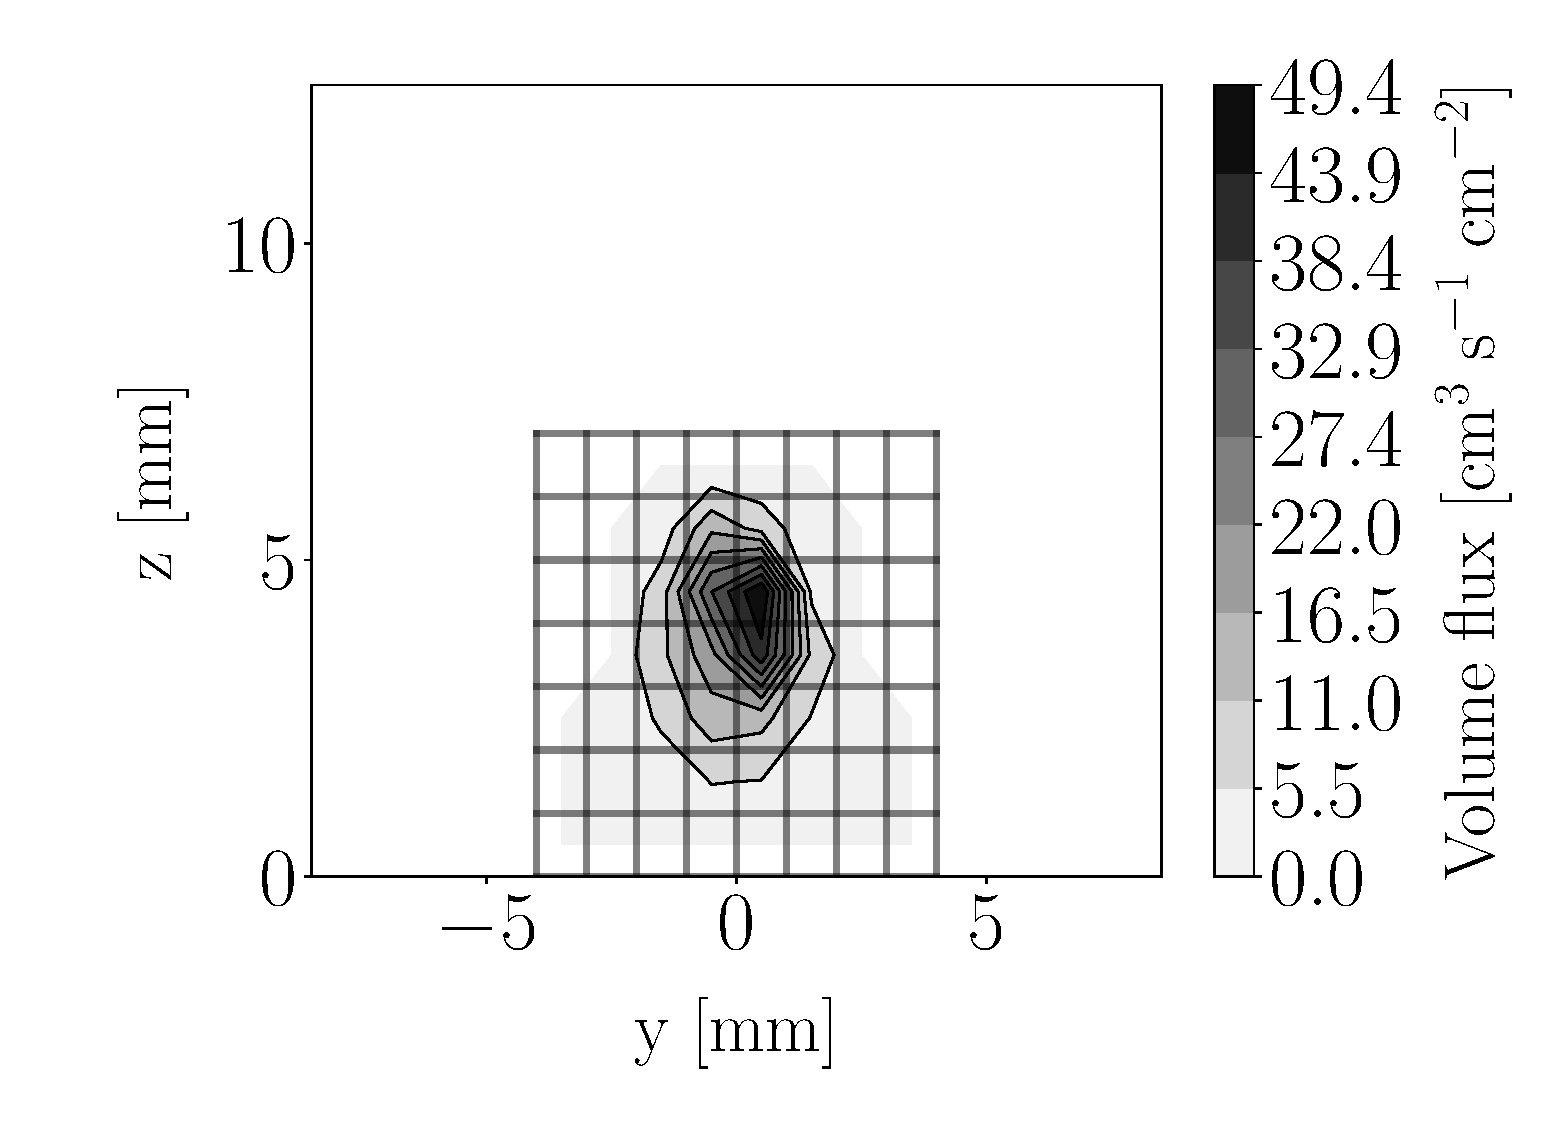
\includegraphics[scale=\scaleSLIJICF]{./part2_developments/figures_ch5_resolved_JICF/injectors_SLI/uG75_dx10_x05_volume_flux_map}
   %\caption{Case UG100\_DX20: filming planes}
   %\label{}
\end{subfigure}
   \hspace{0.17in}
\begin{subfigure}[b]{0.3\textwidth}
	\centering
   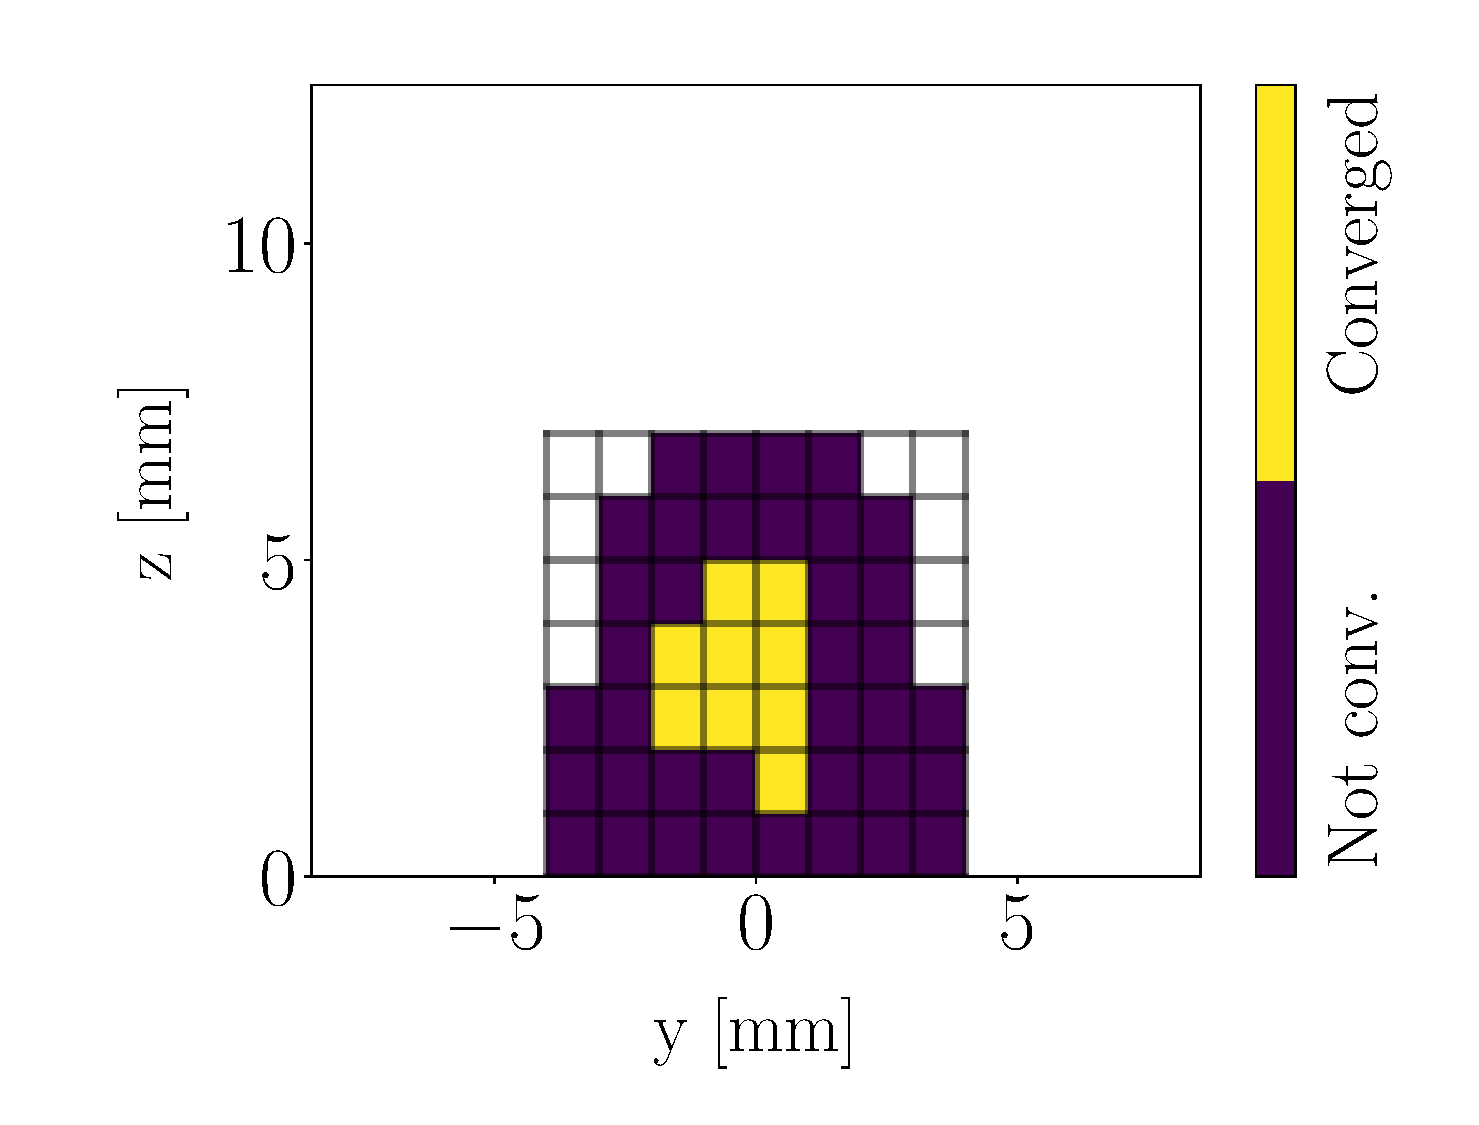
\includegraphics[scale=\scaleSLIJICF]{./part2_developments/figures_ch5_resolved_JICF/injectors_SLI/uG75_dx10_x05_convergence_map}
   %\caption{Case UG100\_DX10: crossflow planes}
   %\label{} 
\end{subfigure}

\vskip\baselineskip

\begin{subfigure}[b]{0.3\textwidth}
	\centering
   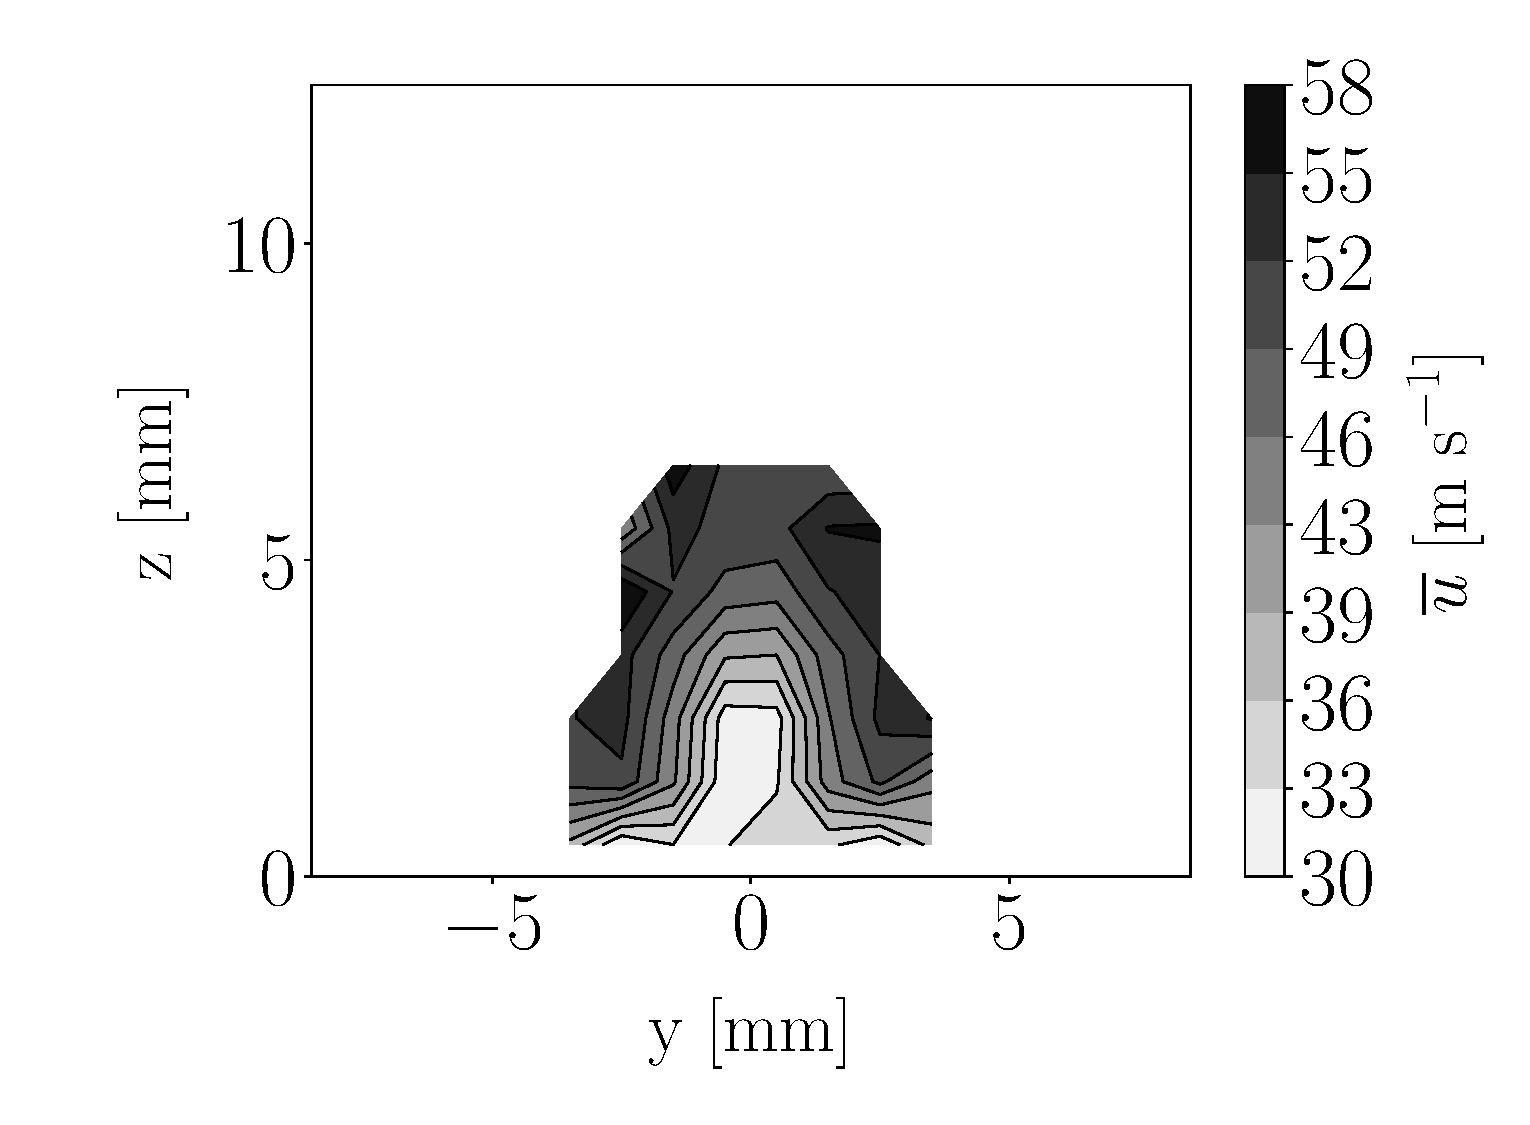
\includegraphics[scale=\scaleSLIJICF]{./part2_developments/figures_ch5_resolved_JICF/injectors_SLI/uG75_dx10_x05_ux_mean_map}
   %\caption{Case UG100\_DX20: crossflow planes}
   %\label{} 
\end{subfigure}
   \hspace{0.17in}
\begin{subfigure}[b]{0.3\textwidth}
	\centering
   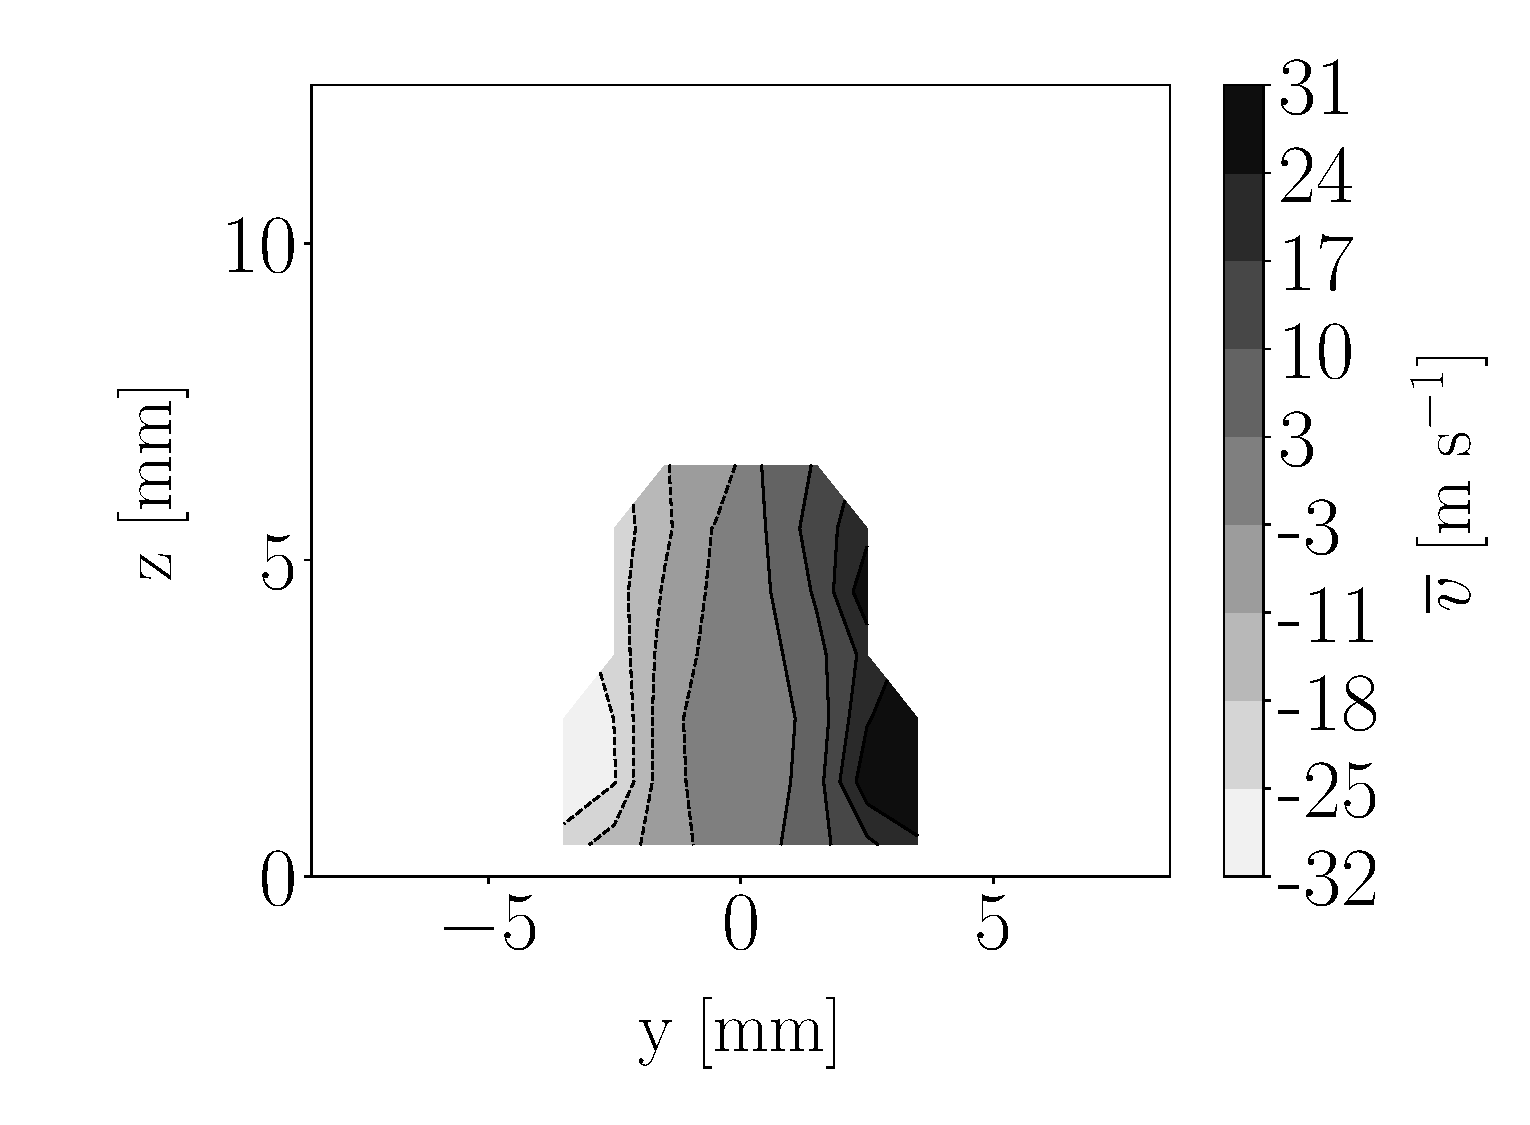
\includegraphics[scale=\scaleSLIJICF]{./part2_developments/figures_ch5_resolved_JICF/injectors_SLI/uG75_dx10_x05_uy_mean_map}
   %\caption{Case UG100\_DX20: filming planes}
   %\label{}
\end{subfigure}
   \hspace{0.17in}
\begin{subfigure}[b]{0.3\textwidth}
	\centering
   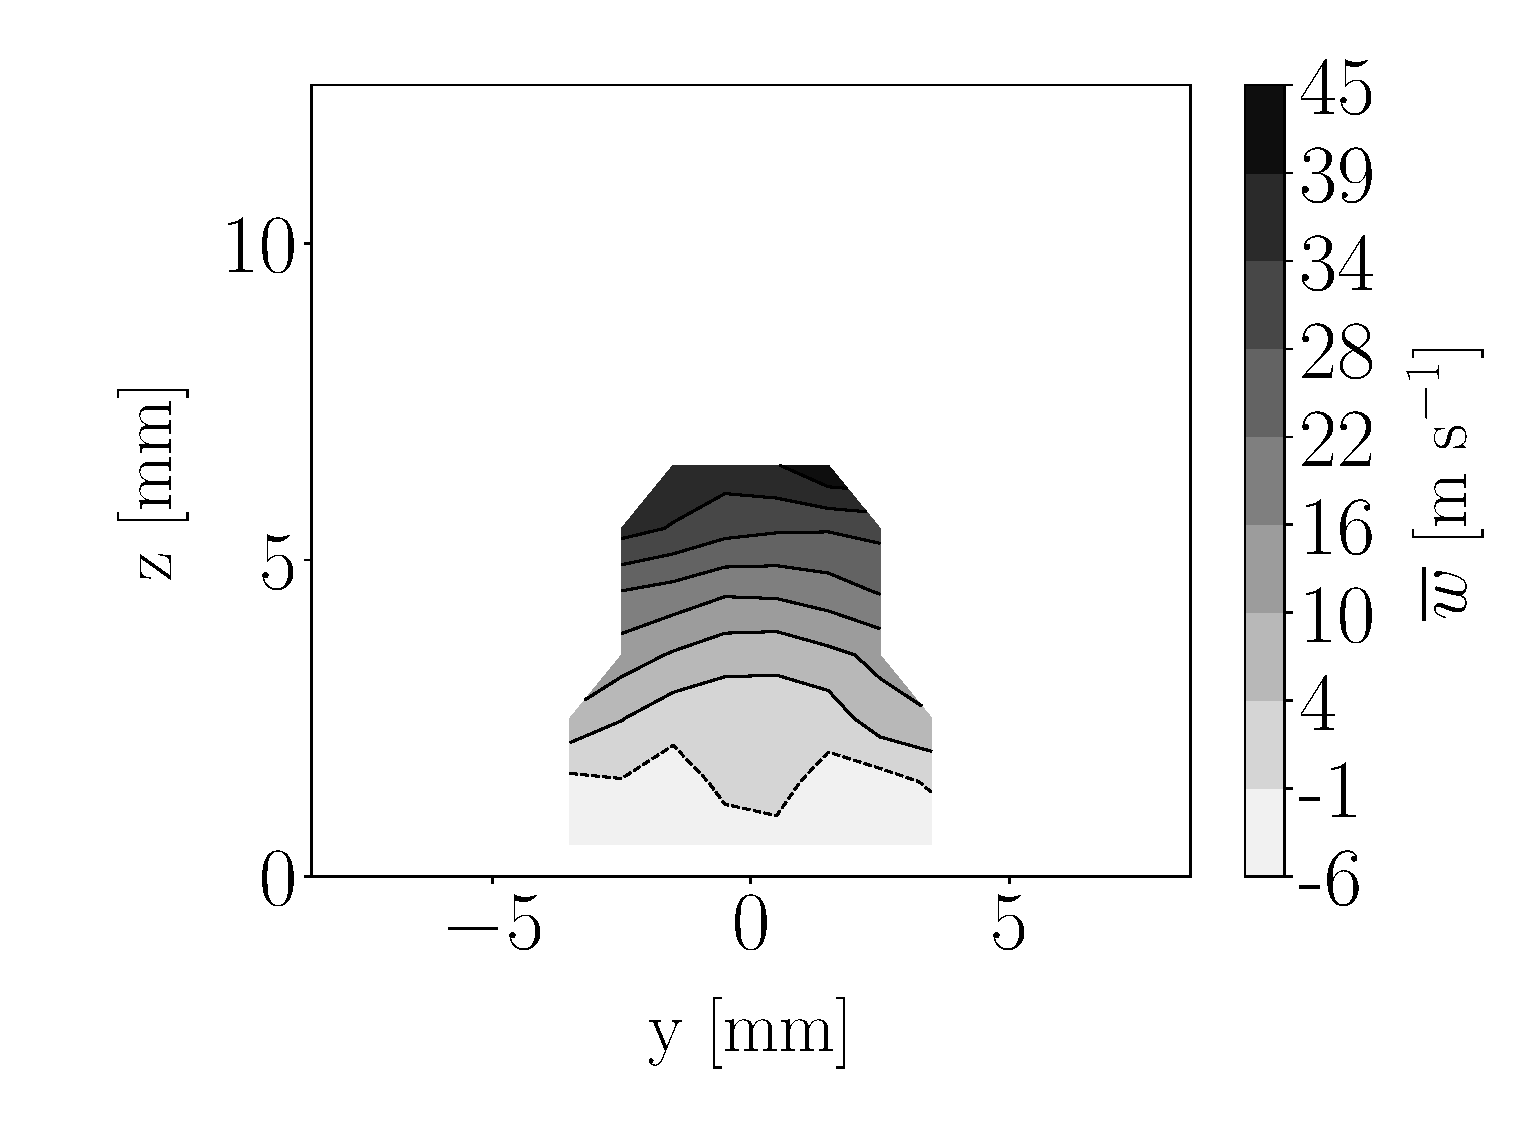
\includegraphics[scale=\scaleSLIJICF]{./part2_developments/figures_ch5_resolved_JICF/injectors_SLI/uG75_dx10_x05_uz_mean_map}
   %\caption{Case UG100\_DX10: crossflow planes}
   %\label{} 
\end{subfigure}
\caption{Spray states at x = 5 mm for case UG75\_DX10}
\label{fig:injectors_sli_uG75_dx10_x05}
\end{figure}


%%%%%%%%%%%%%%%% UG75_DX10, x = 10 mm


\begin{figure}[h!]
\centering
\begin{subfigure}[b]{0.3\textwidth}
	\centering
   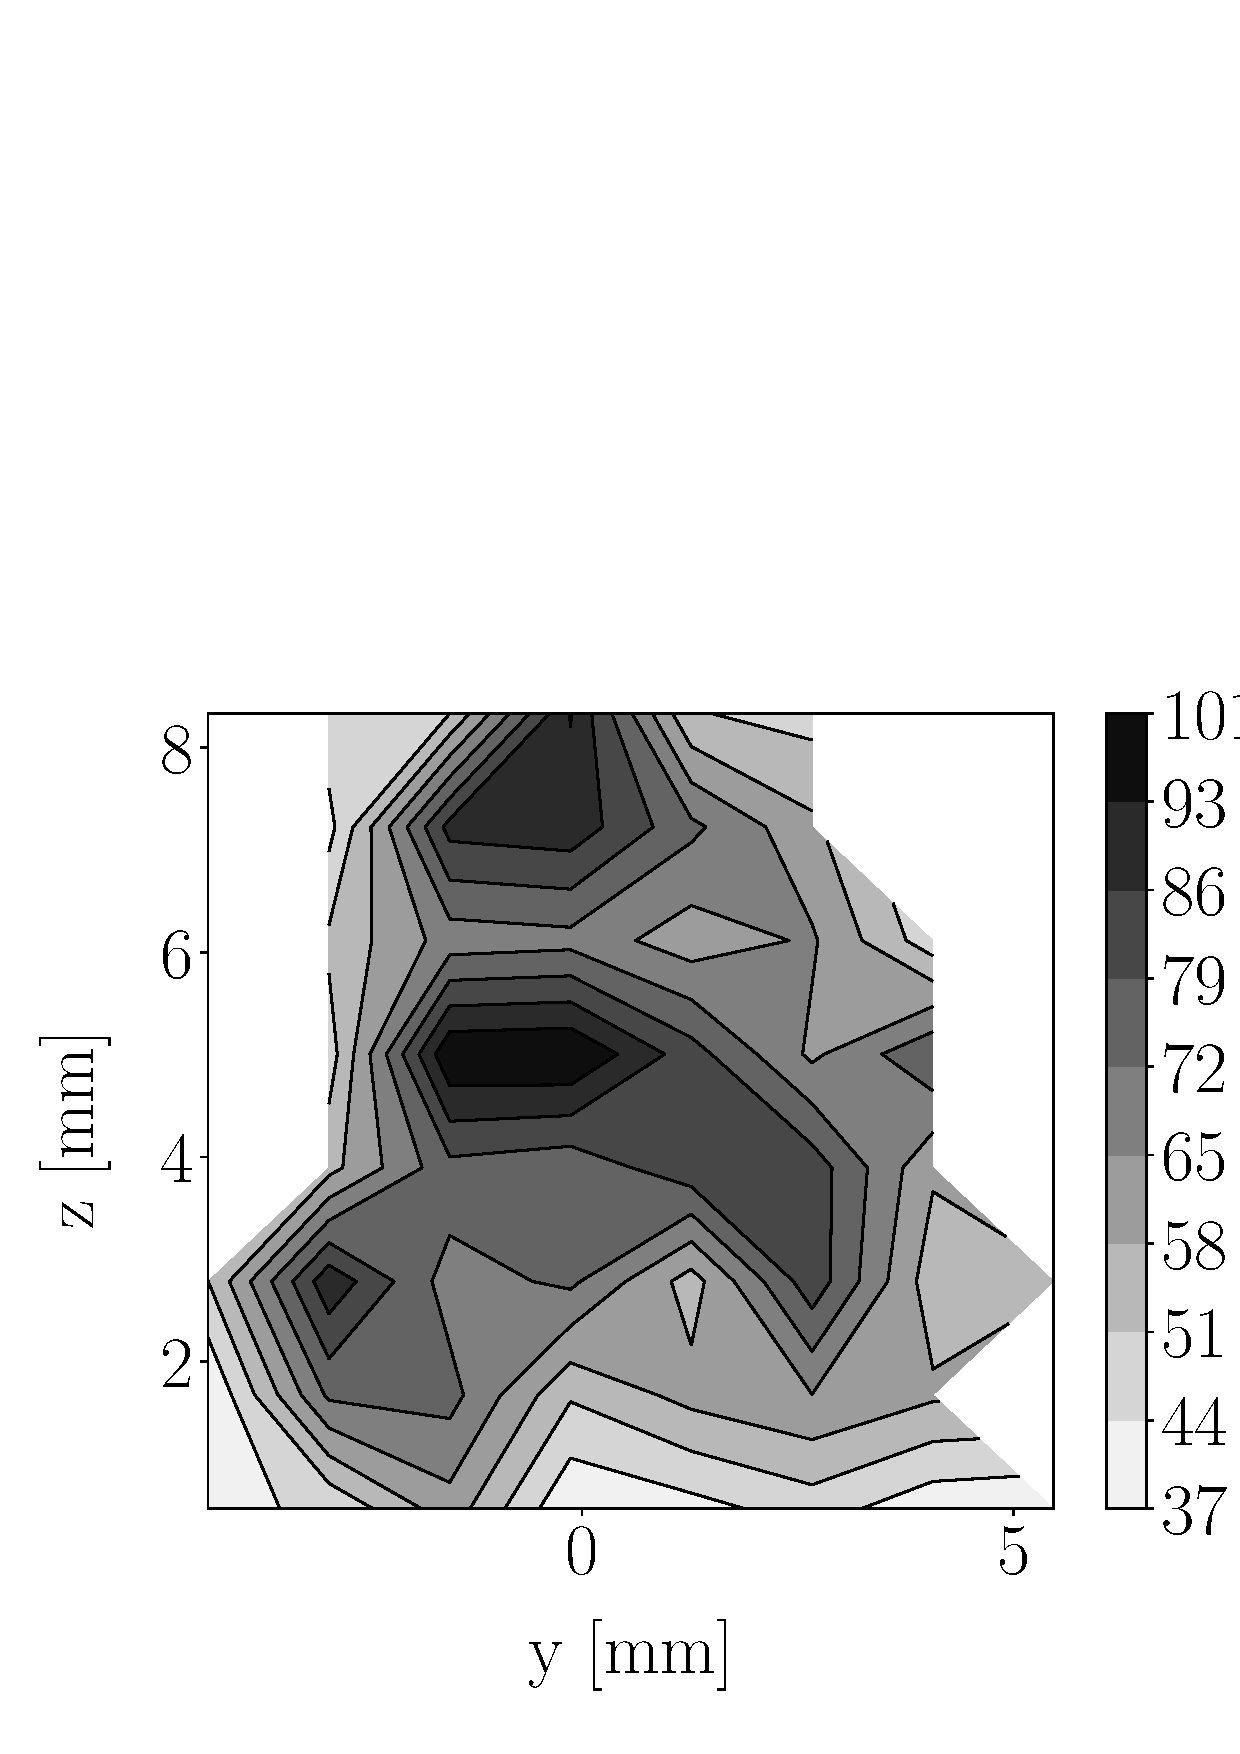
\includegraphics[scale=\scaleSLIJICF]{./part2_developments/figures_ch5_resolved_JICF/injectors_SLI/uG75_dx10_x10_SMD_map}
   %\caption{Case UG100\_DX20: crossflow planes}
   %\label{} 
\end{subfigure}
   \hspace{0.17in}
\begin{subfigure}[b]{0.3\textwidth}
	\centering
   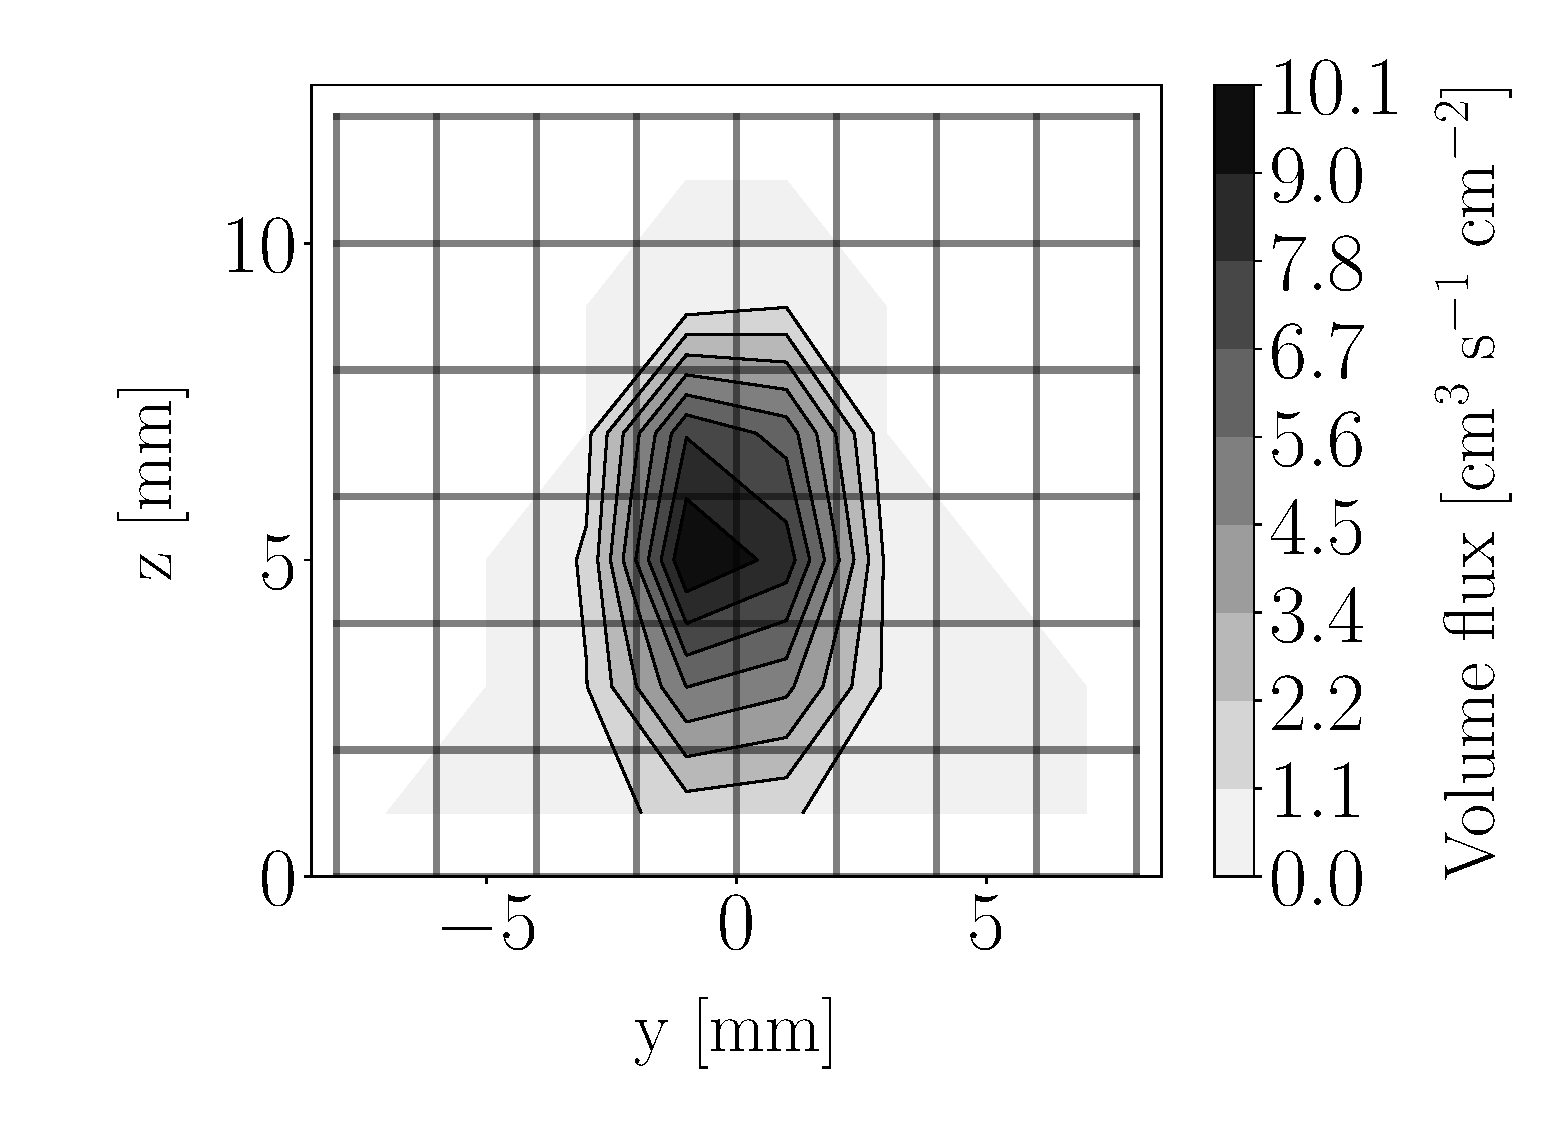
\includegraphics[scale=\scaleSLIJICF]{./part2_developments/figures_ch5_resolved_JICF/injectors_SLI/uG75_dx10_x10_volume_flux_map}
   %\caption{Case UG100\_DX20: filming planes}
   %\label{}
\end{subfigure}
   \hspace{0.17in}
\begin{subfigure}[b]{0.3\textwidth}
	\centering
   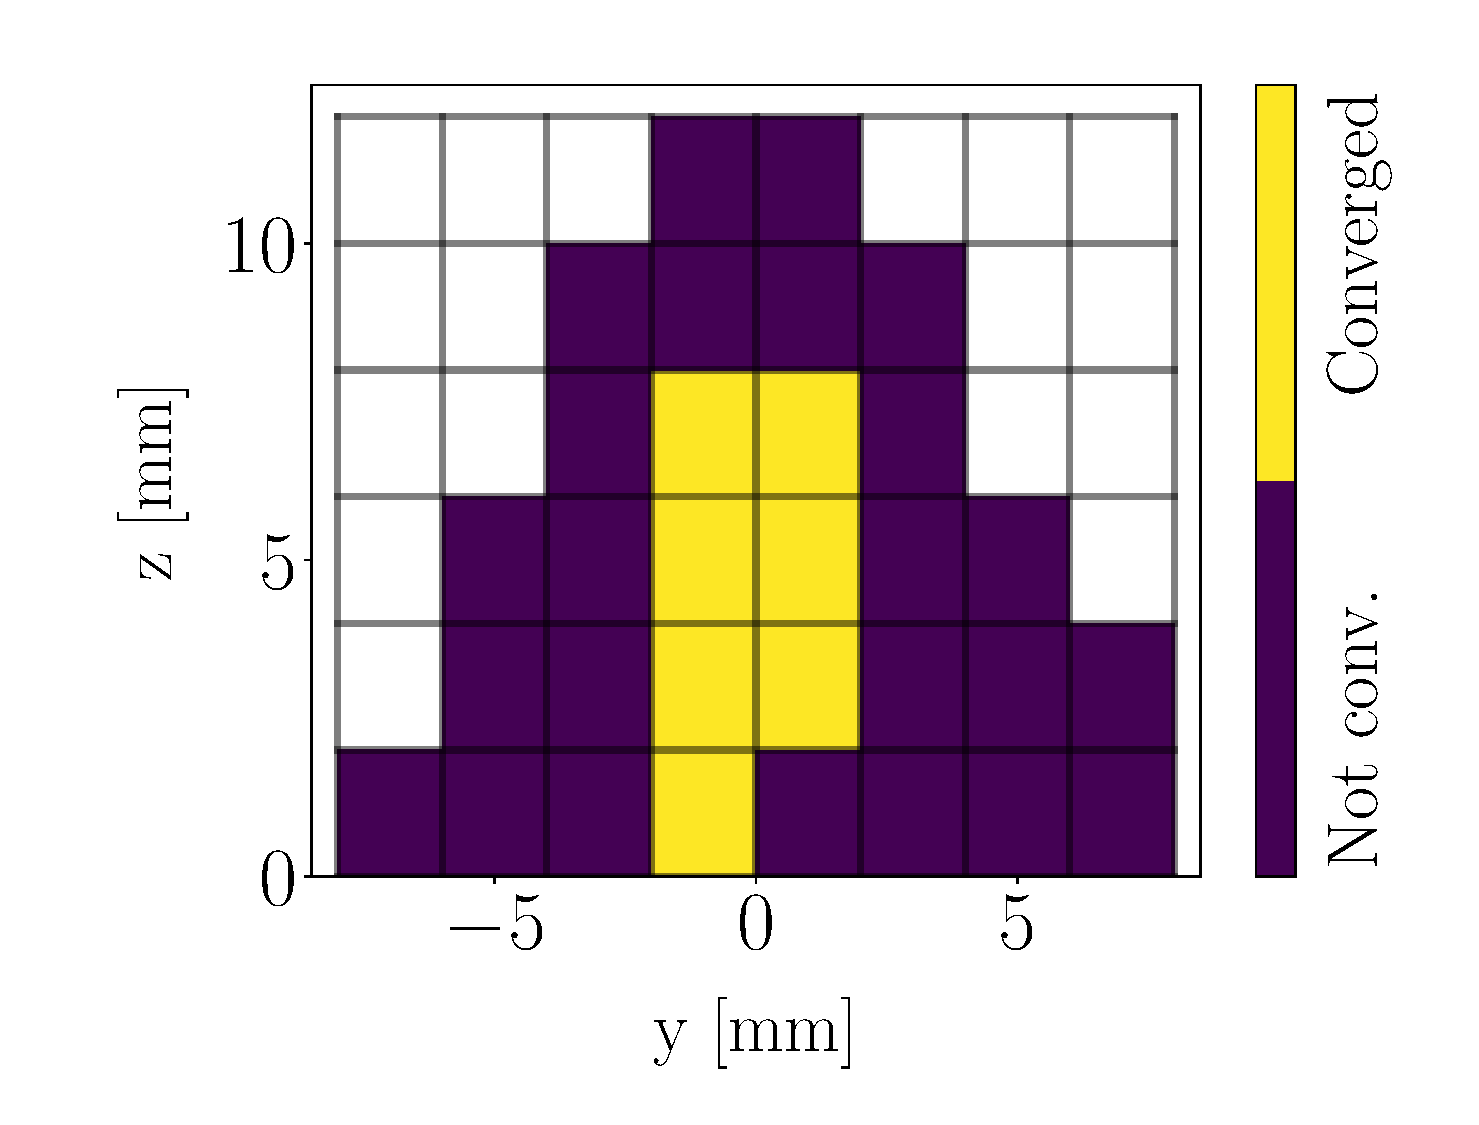
\includegraphics[scale=\scaleSLIJICF]{./part2_developments/figures_ch5_resolved_JICF/injectors_SLI/uG75_dx10_x10_convergence_map}
   %\caption{Case UG100\_DX10: crossflow planes}
   %\label{} 
\end{subfigure}

\vskip\baselineskip

\begin{subfigure}[b]{0.3\textwidth}
	\centering
   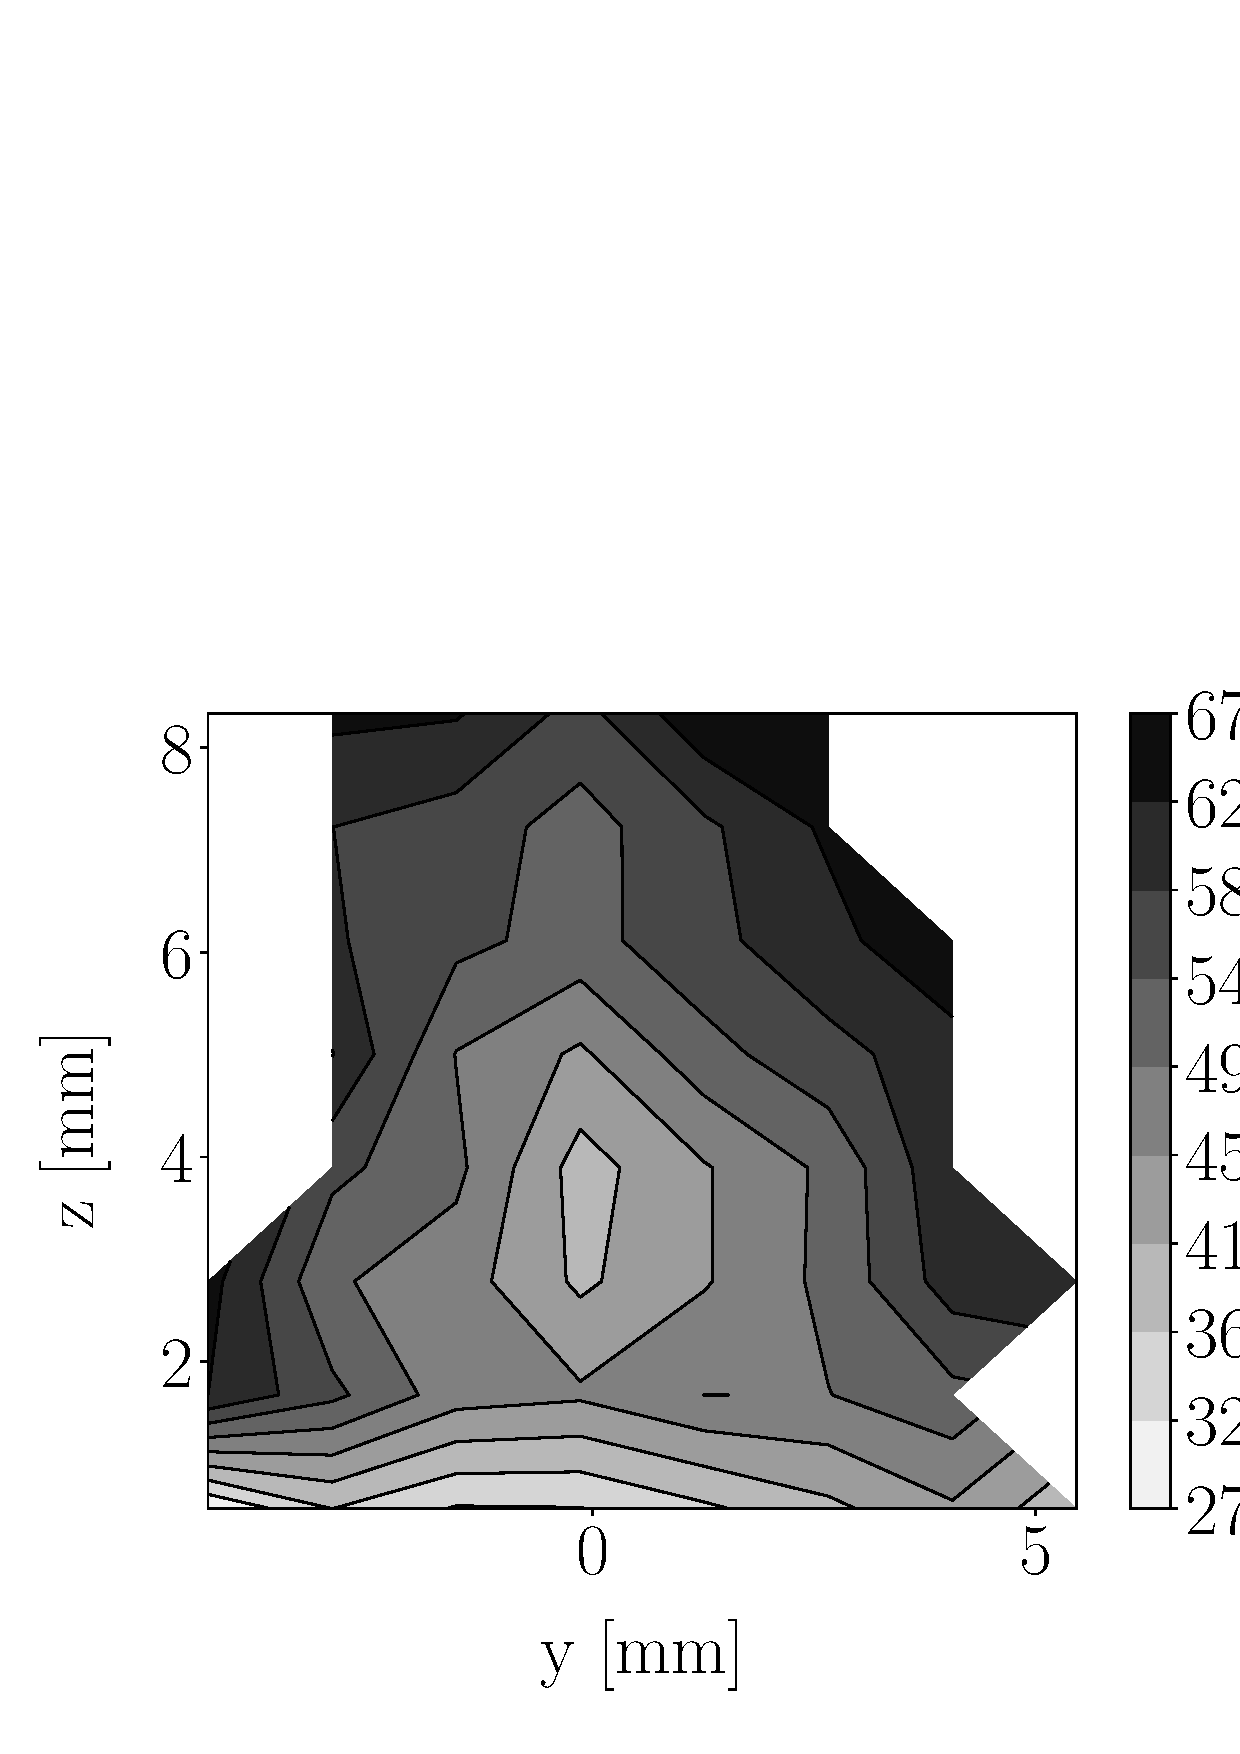
\includegraphics[scale=\scaleSLIJICF]{./part2_developments/figures_ch5_resolved_JICF/injectors_SLI/uG75_dx10_x10_ux_mean_map}
   %\caption{Case UG100\_DX20: crossflow planes}
   %\label{} 
\end{subfigure}
   \hspace{0.17in}
\begin{subfigure}[b]{0.3\textwidth}
	\centering
   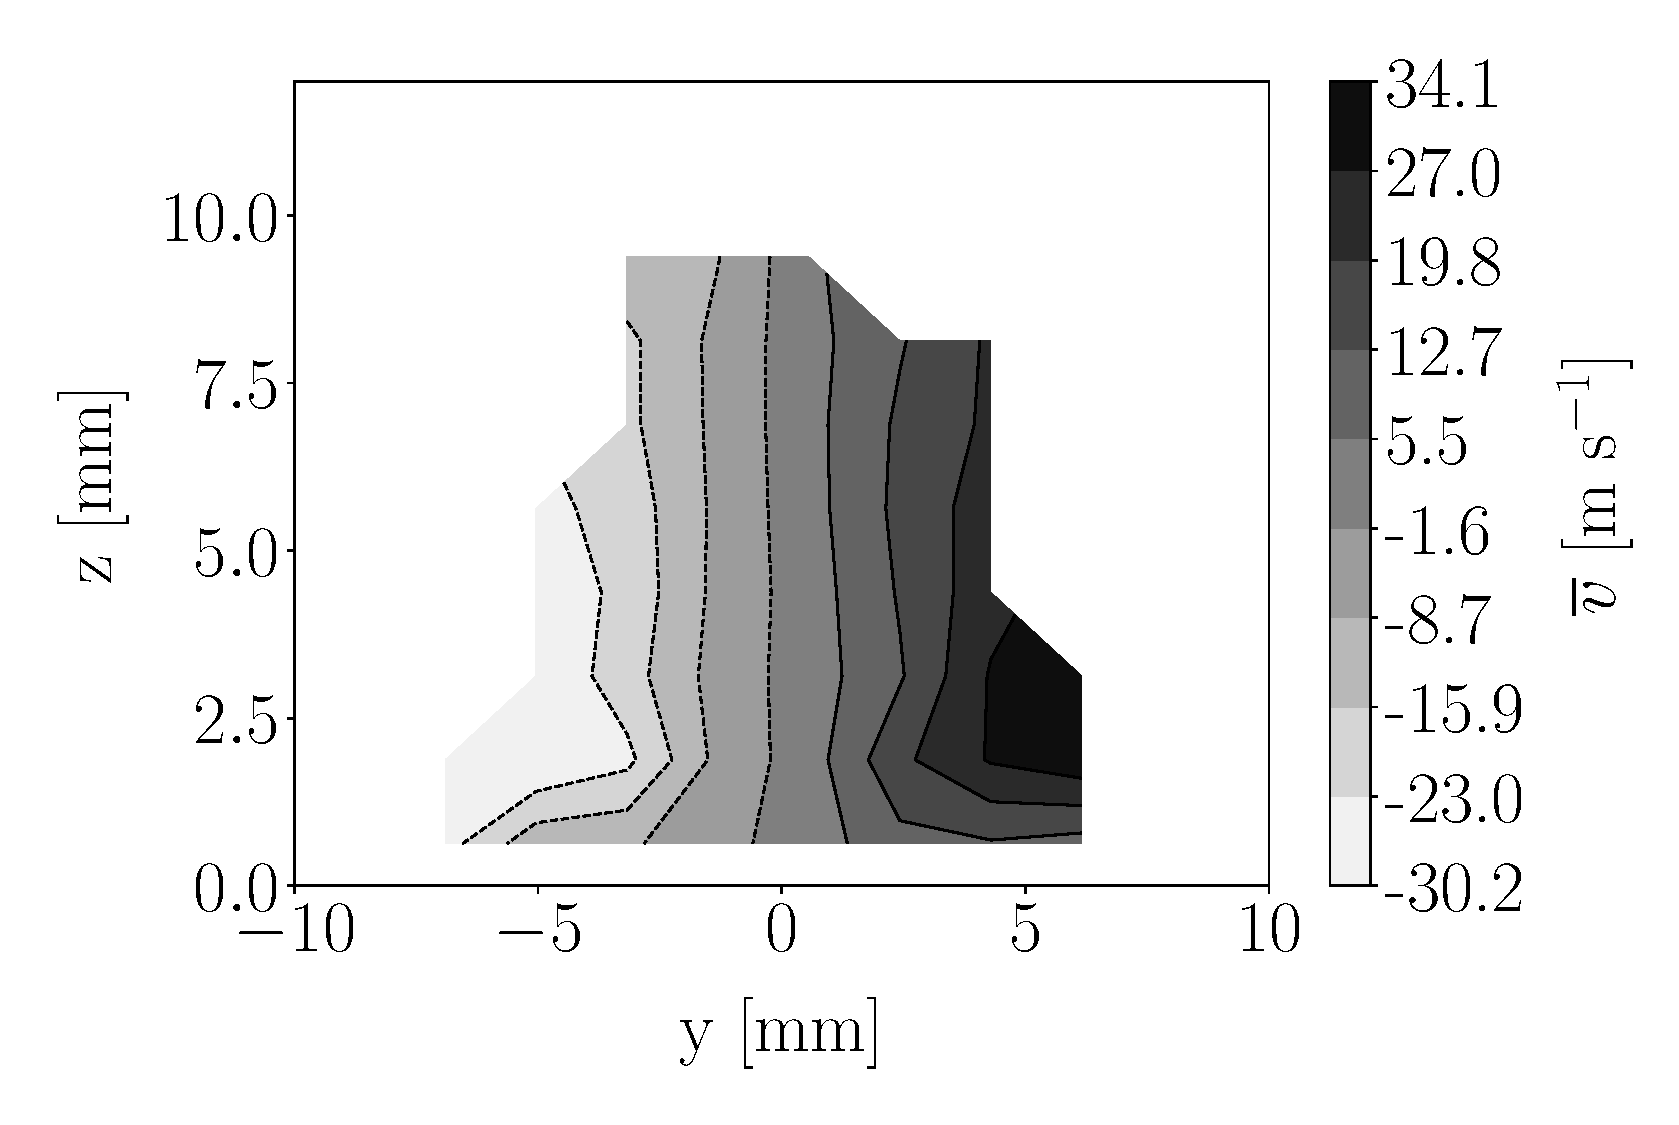
\includegraphics[scale=\scaleSLIJICF]{./part2_developments/figures_ch5_resolved_JICF/injectors_SLI/uG75_dx10_x10_uy_mean_map}
   %\caption{Case UG100\_DX20: filming planes}
   %\label{}
\end{subfigure}
   \hspace{0.17in}
\begin{subfigure}[b]{0.3\textwidth}
	\centering
   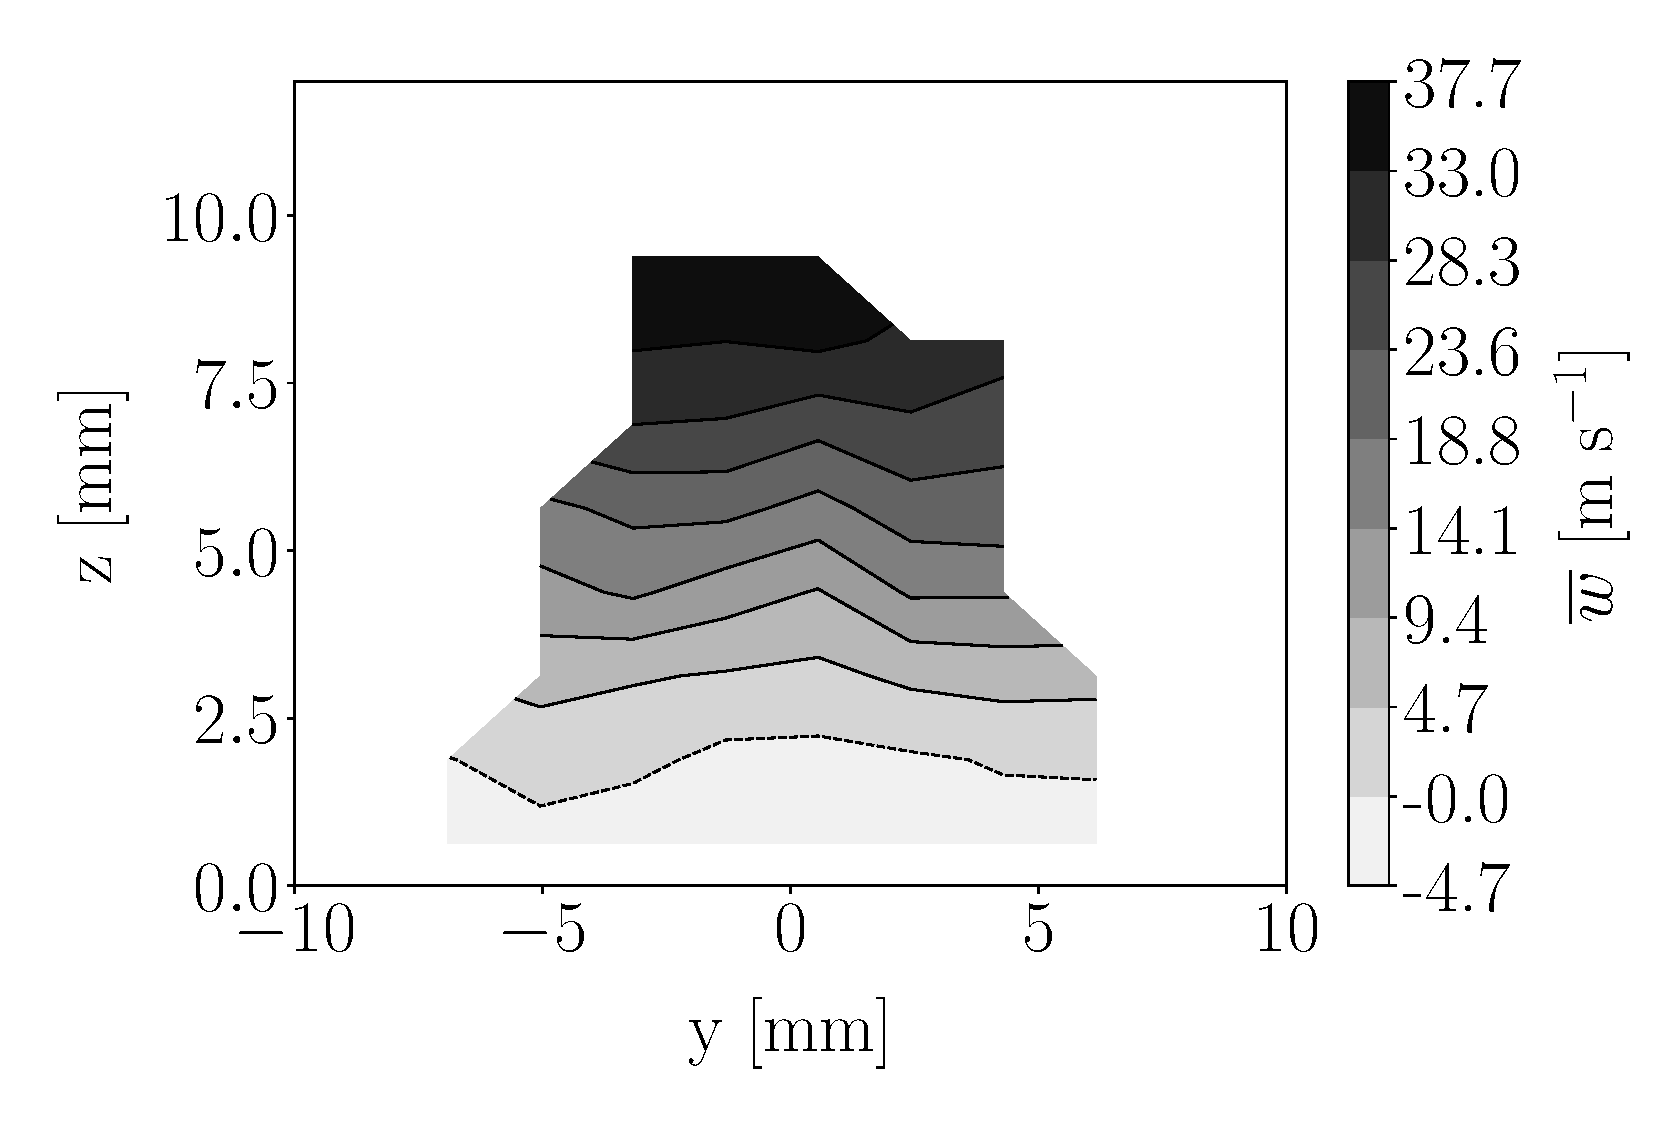
\includegraphics[scale=\scaleSLIJICF]{./part2_developments/figures_ch5_resolved_JICF/injectors_SLI/uG75_dx10_x10_uz_mean_map}
   %\caption{Case UG100\_DX10: crossflow planes}
   %\label{} 
\end{subfigure}
\caption{Spray states at x = 10 mm for case UG75\_DX10}
\label{fig:injectors_sli_uG75_dx10_x10}
\end{figure}


\clearpage

\subsubsection*{Case UG75\_DX20}


%%%%%%%%%%%%%%%% UG75_DX20, x = 5 mm


\begin{figure}[h!]
\centering
\begin{subfigure}[b]{0.3\textwidth}
	\centering
   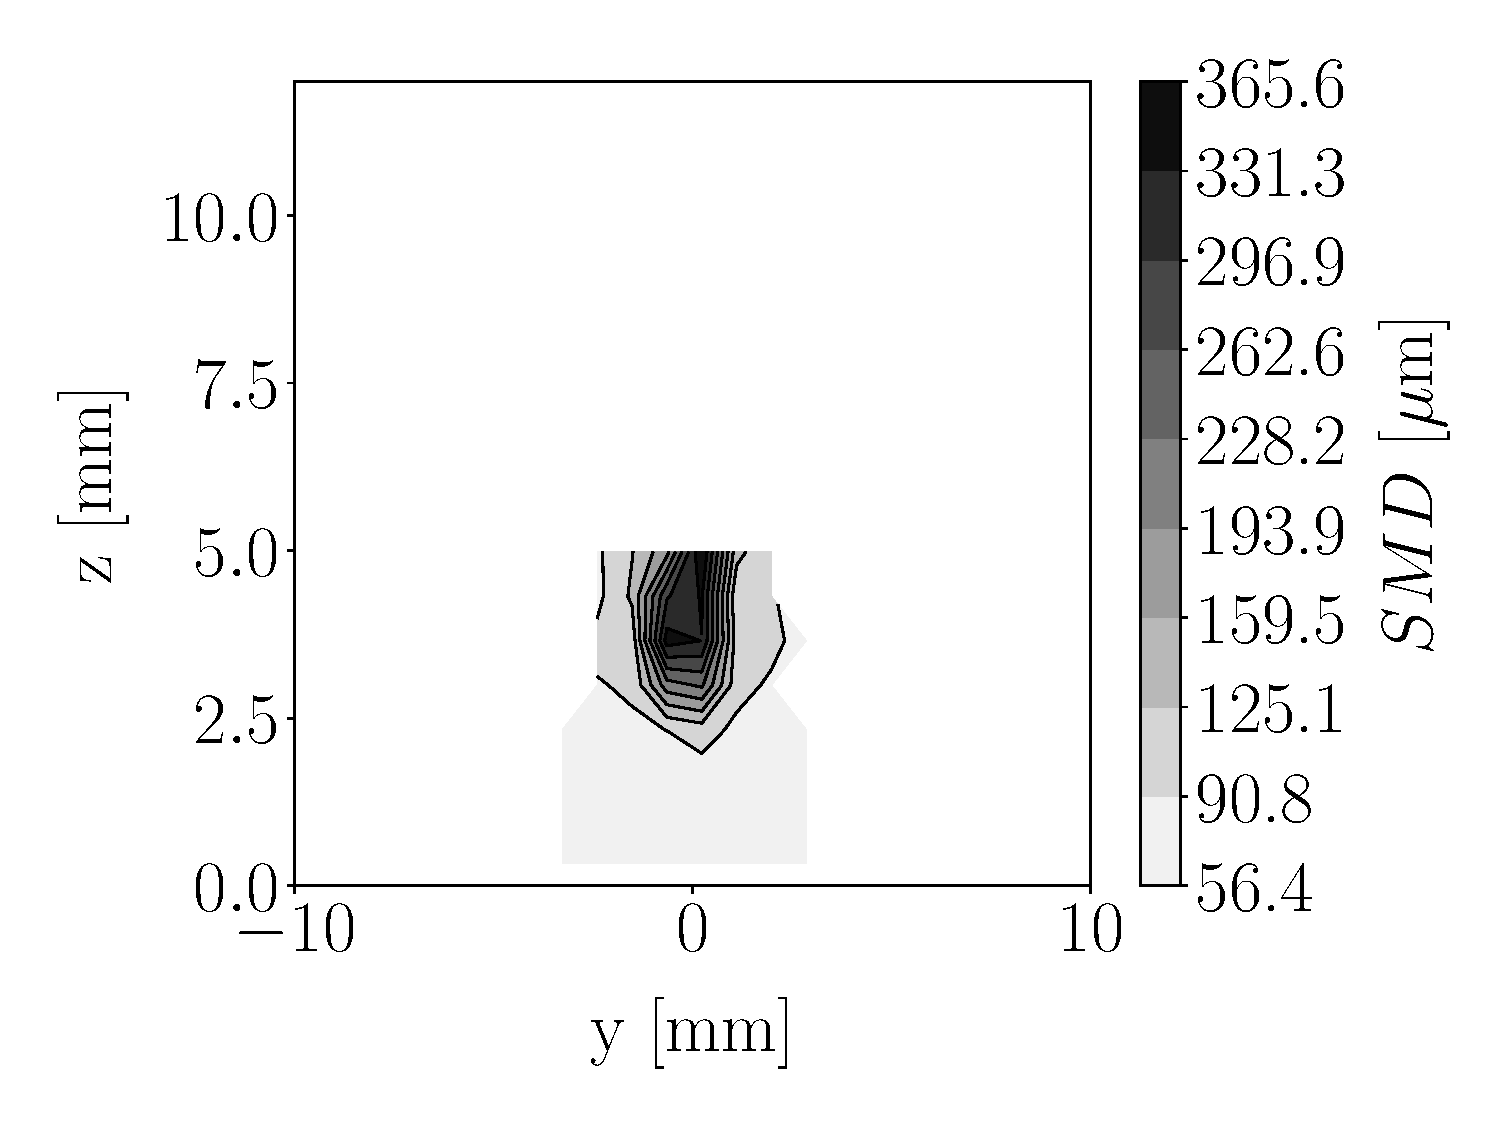
\includegraphics[scale=\scaleSLIJICF]{./part2_developments/figures_ch5_resolved_JICF/injectors_SLI/uG75_dx20_x05_SMD_map}
   %\caption{Case UG100\_DX20: crossflow planes}
   %\label{} 
\end{subfigure}
   \hspace{0.17in}
\begin{subfigure}[b]{0.3\textwidth}
	\centering
   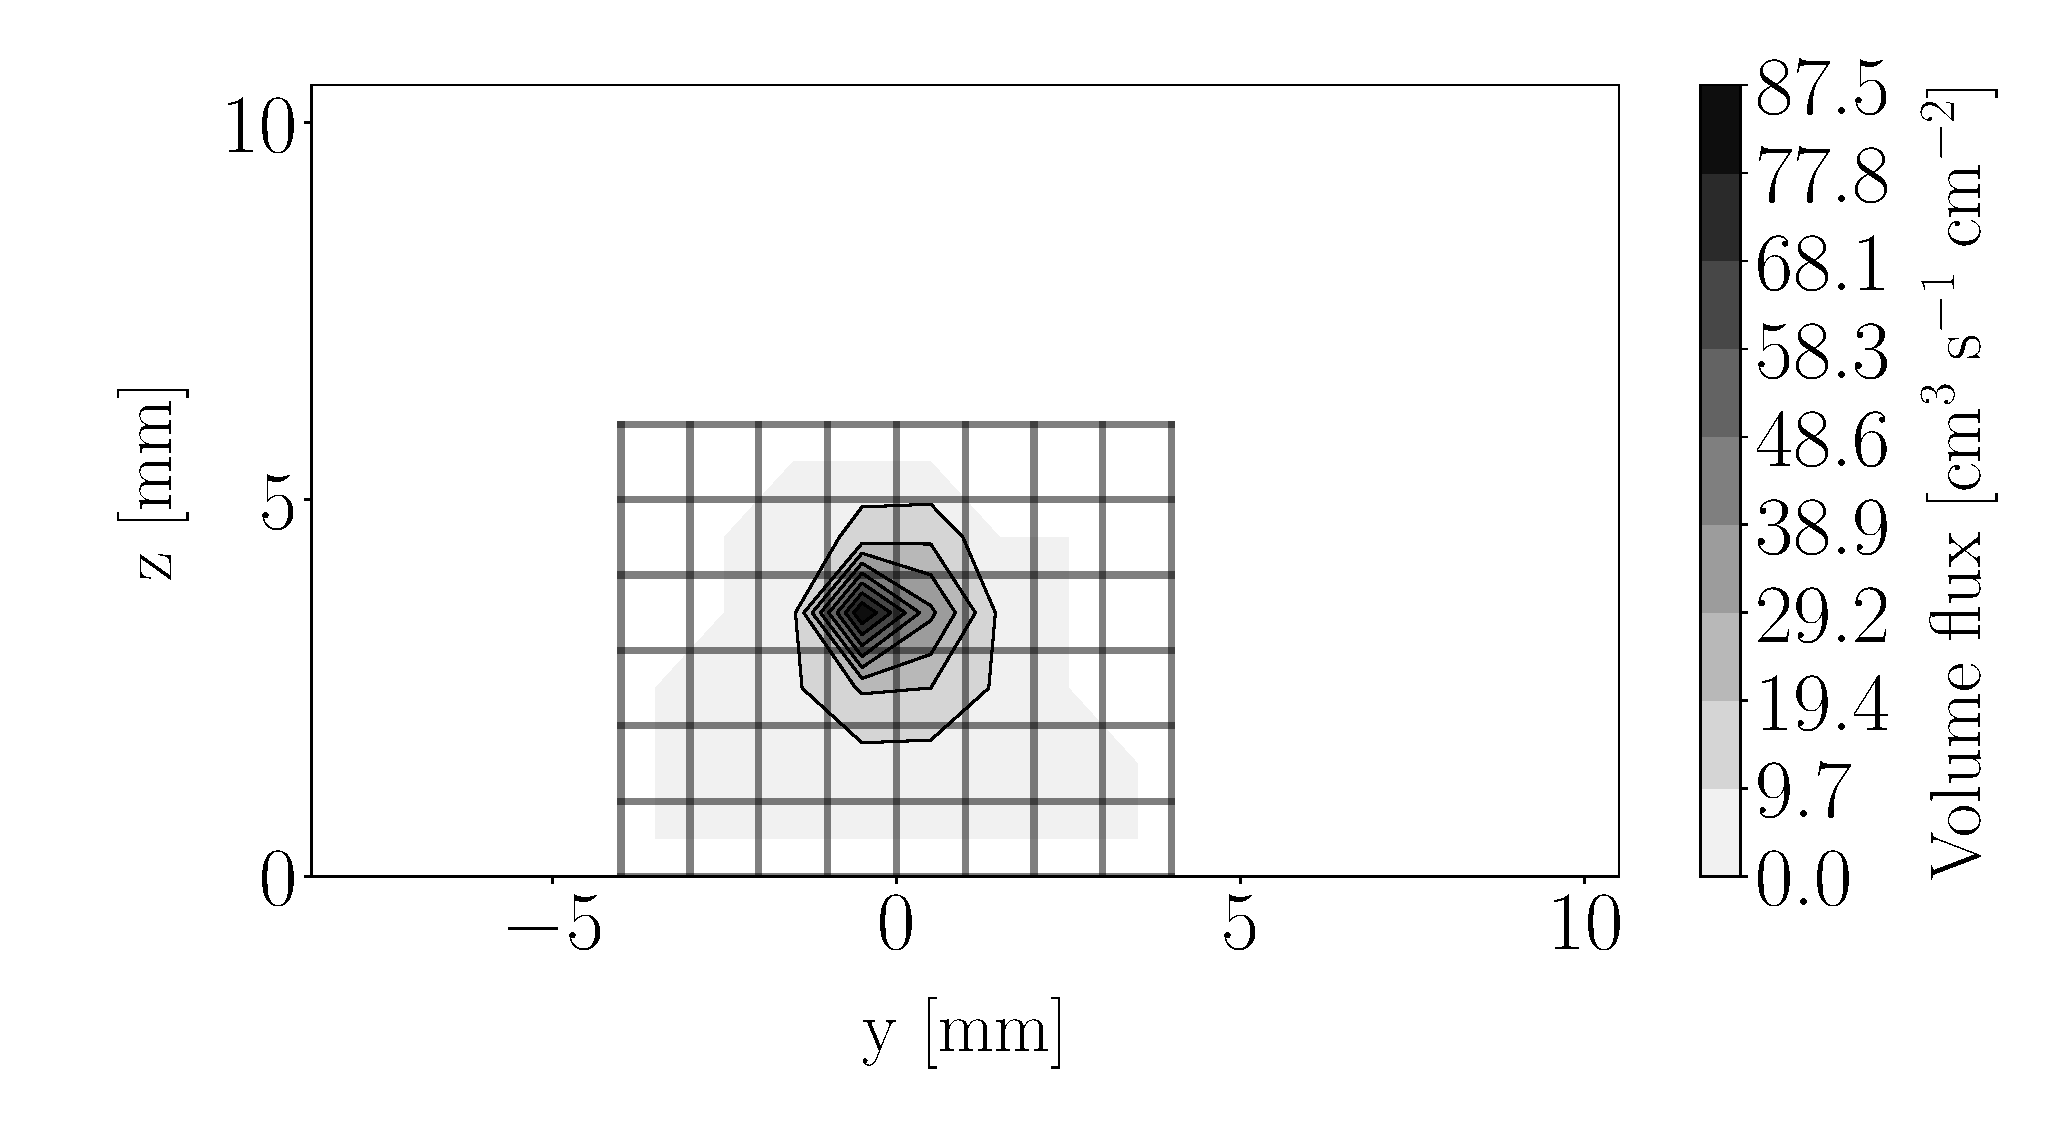
\includegraphics[scale=\scaleSLIJICF]{./part2_developments/figures_ch5_resolved_JICF/injectors_SLI/uG75_dx20_x05_volume_flux_map}
   %\caption{Case UG100\_DX20: filming planes}
   %\label{}
\end{subfigure}
   \hspace{0.17in}
\begin{subfigure}[b]{0.3\textwidth}
	\centering
   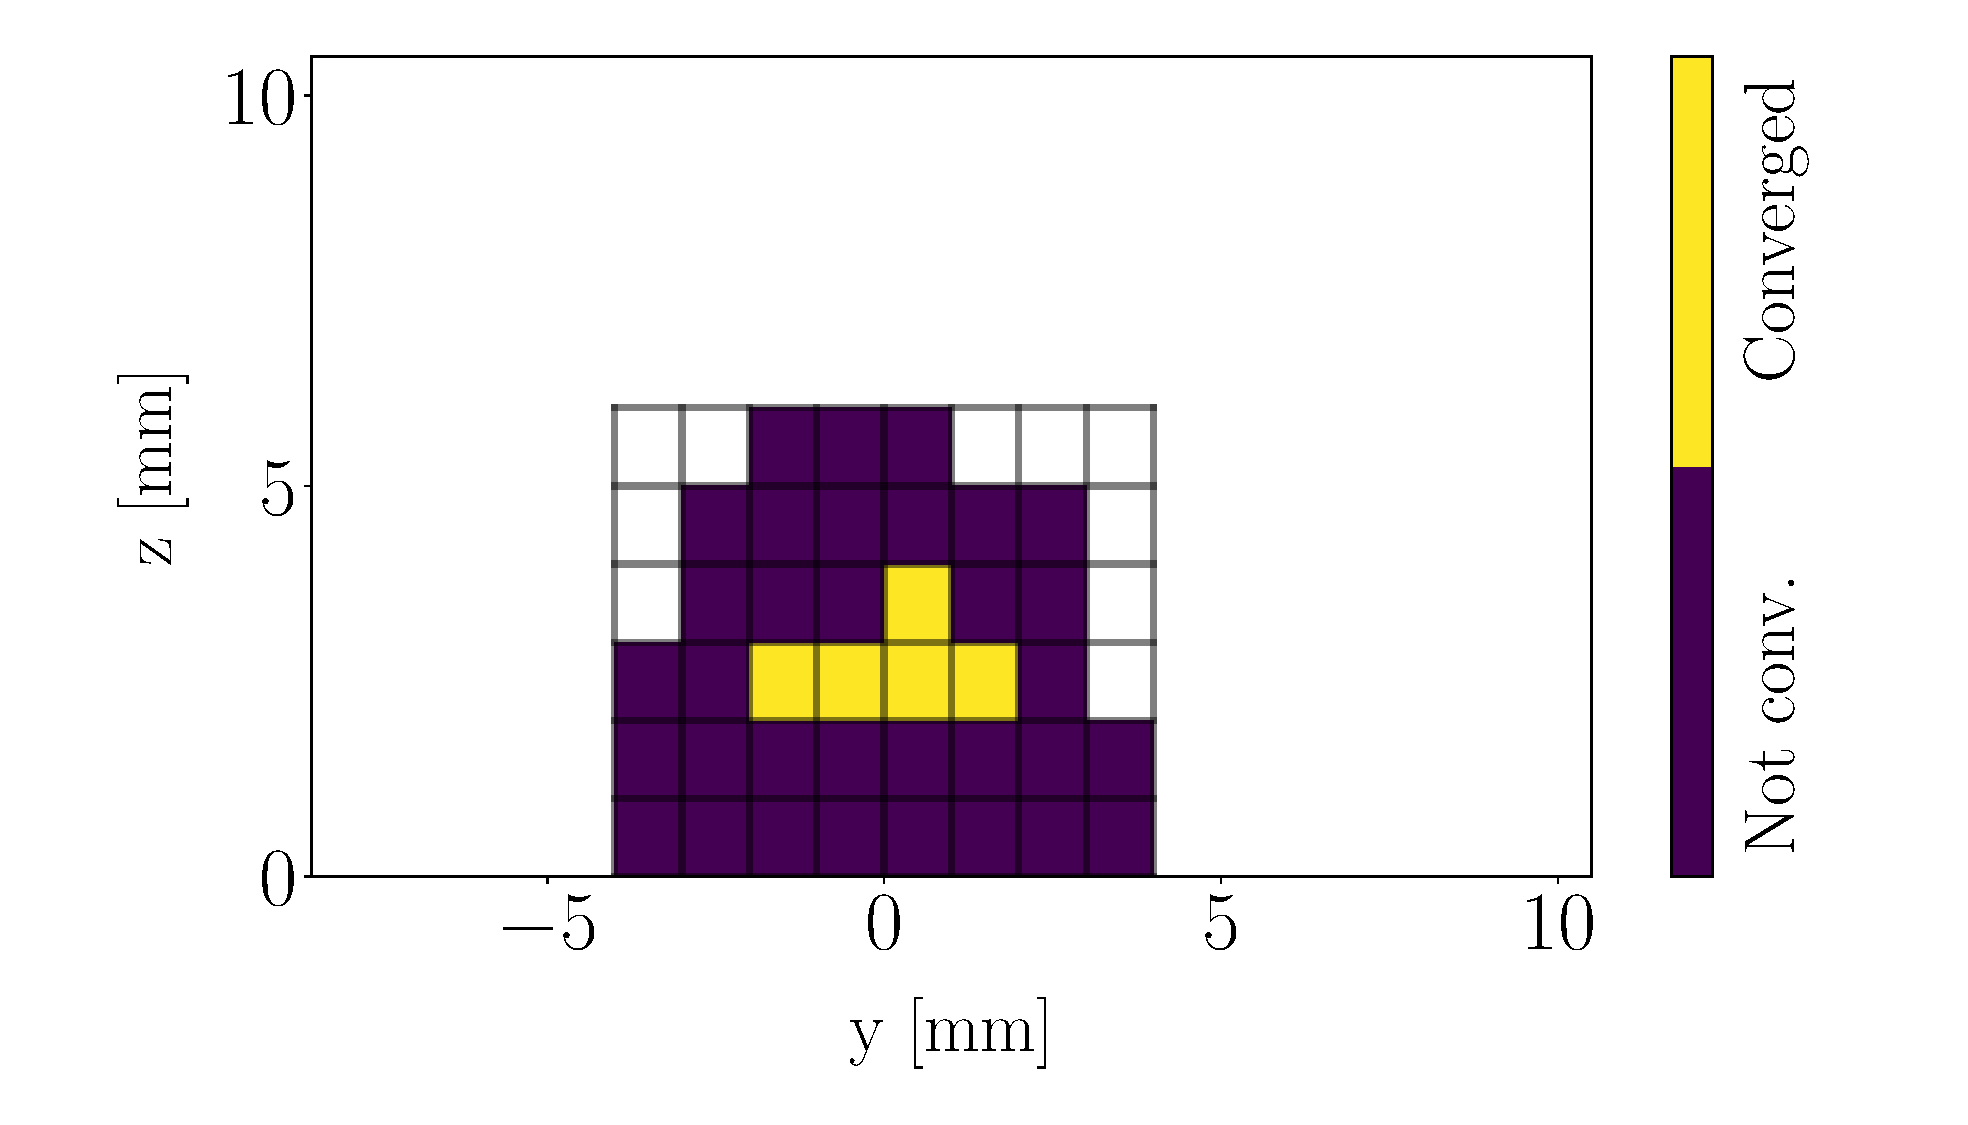
\includegraphics[scale=\scaleSLIJICF]{./part2_developments/figures_ch5_resolved_JICF/injectors_SLI/uG75_dx20_x05_convergence_map}
   %\caption{Case UG100\_DX10: crossflow planes}
   %\label{} 
\end{subfigure}

\vskip\baselineskip

\begin{subfigure}[b]{0.3\textwidth}
	\centering
   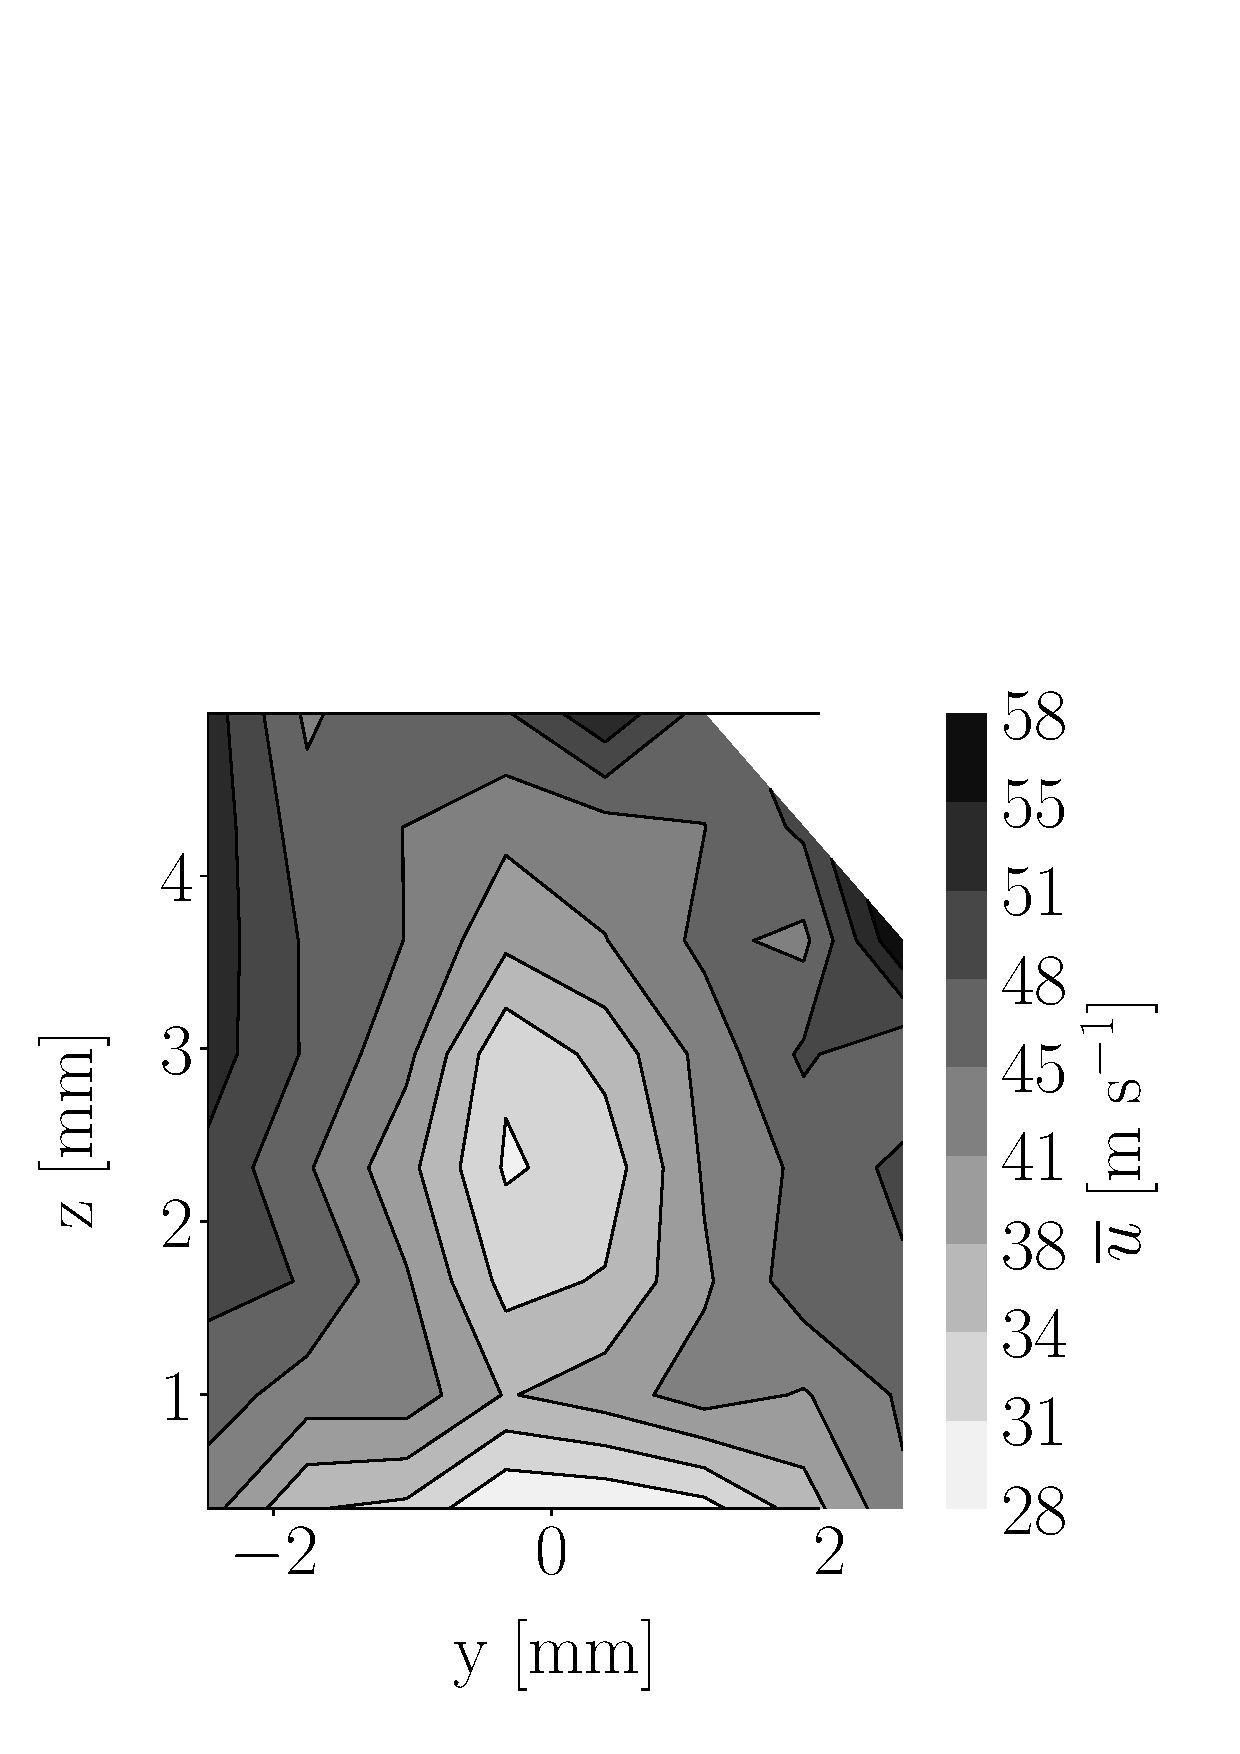
\includegraphics[scale=\scaleSLIJICF]{./part2_developments/figures_ch5_resolved_JICF/injectors_SLI/uG75_dx20_x05_ux_mean_map}
   %\caption{Case UG100\_DX20: crossflow planes}
   %\label{} 
\end{subfigure}
   \hspace{0.17in}
\begin{subfigure}[b]{0.3\textwidth}
	\centering
   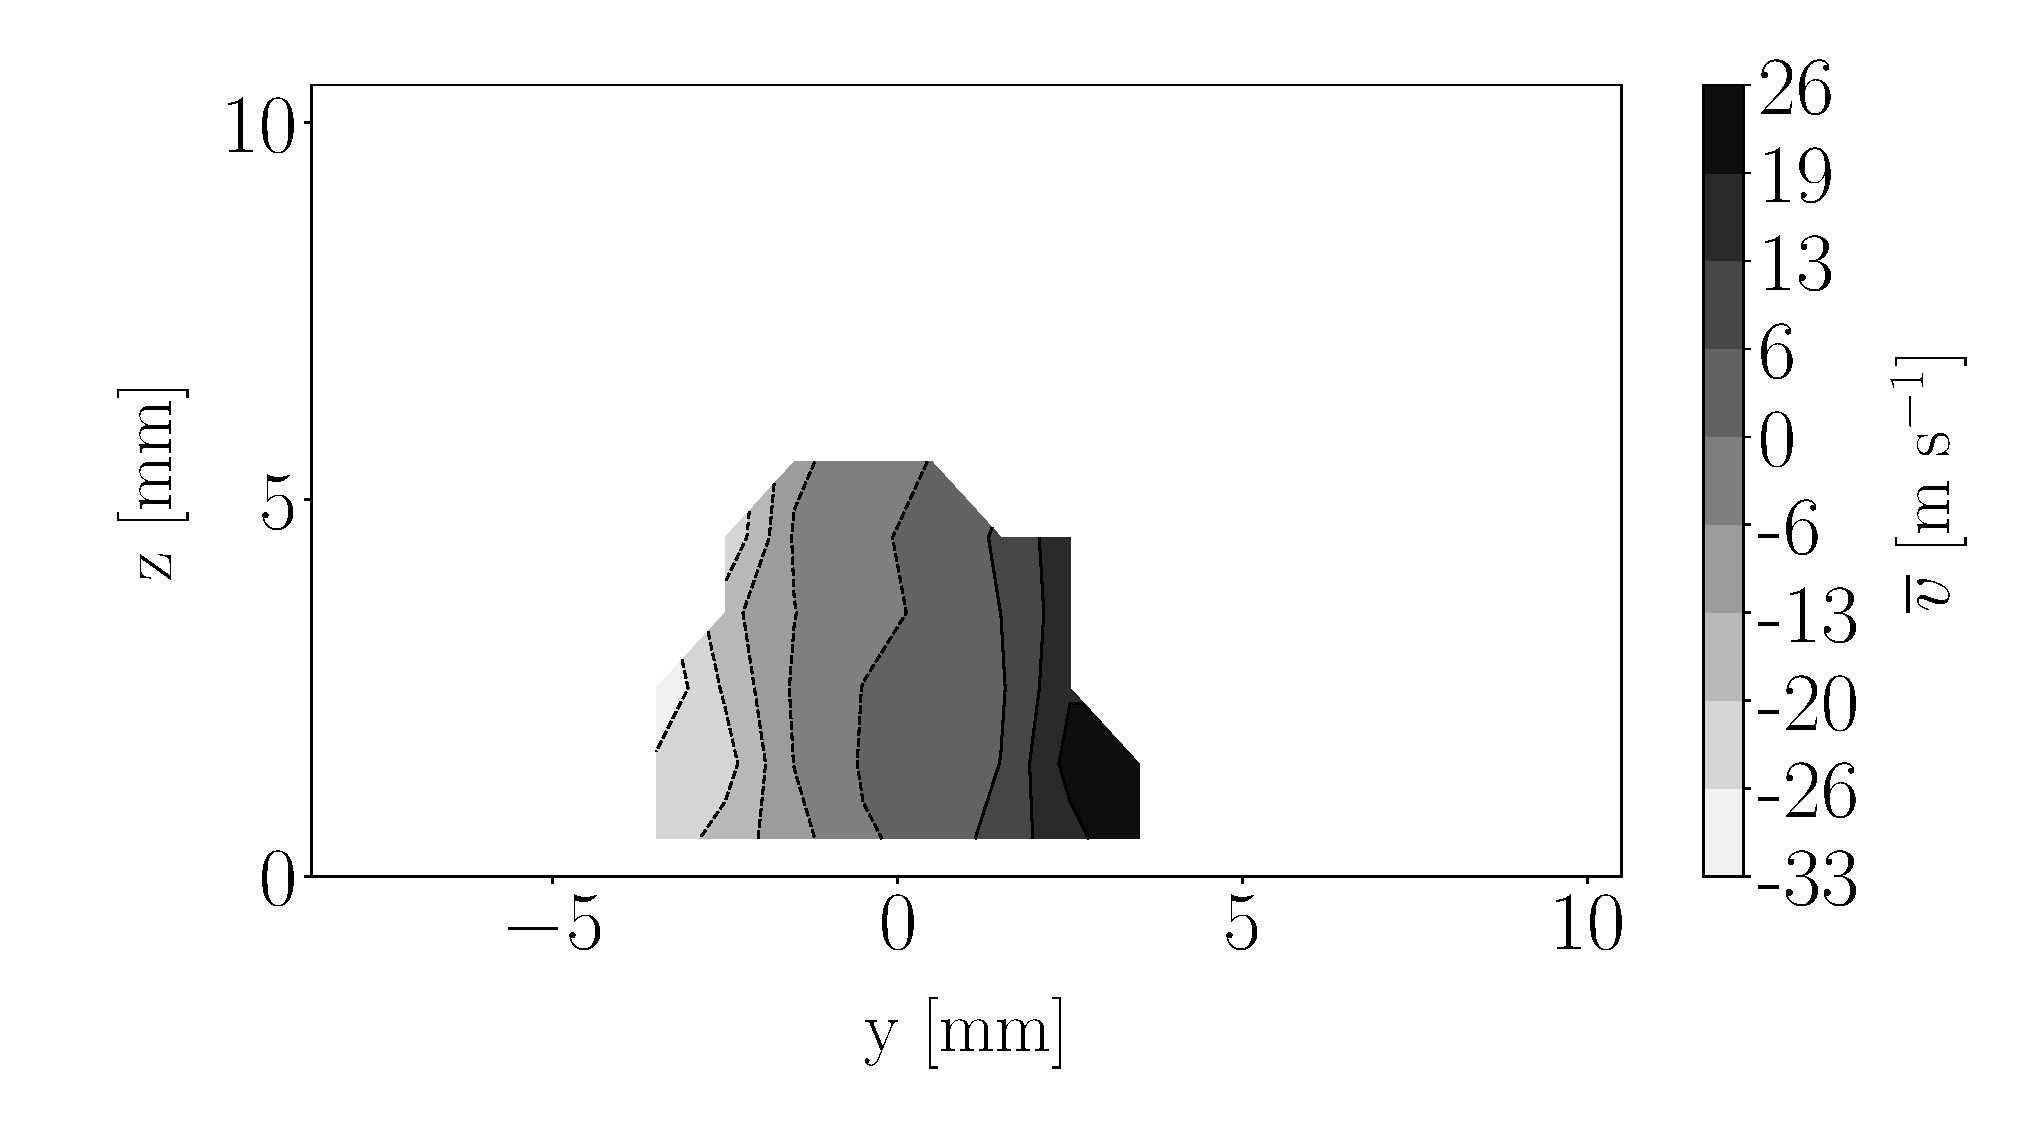
\includegraphics[scale=\scaleSLIJICF]{./part2_developments/figures_ch5_resolved_JICF/injectors_SLI/uG75_dx20_x05_uy_mean_map}
   %\caption{Case UG100\_DX20: filming planes}
   %\label{}
\end{subfigure}
   \hspace{0.17in}
\begin{subfigure}[b]{0.3\textwidth}
	\centering
   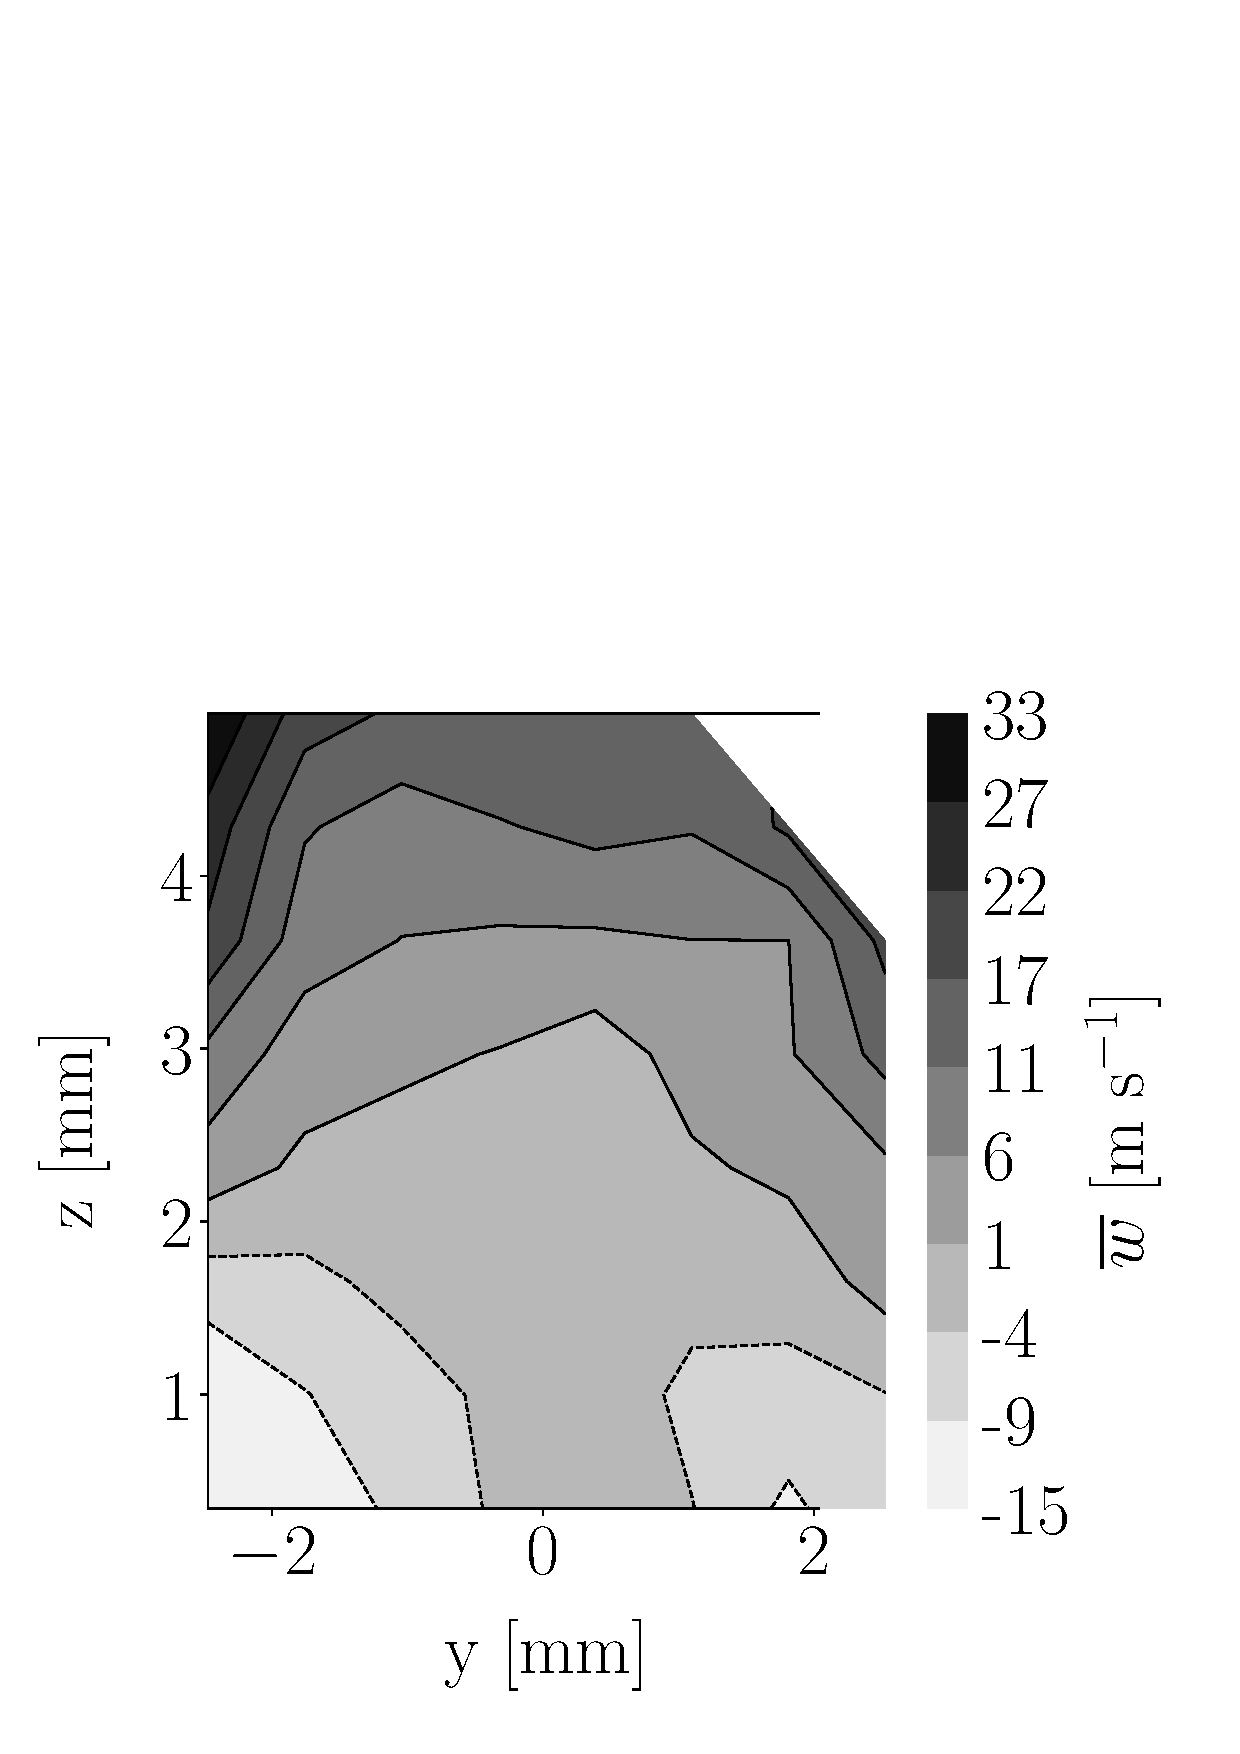
\includegraphics[scale=\scaleSLIJICF]{./part2_developments/figures_ch5_resolved_JICF/injectors_SLI/uG75_dx20_x05_uz_mean_map}
   %\caption{Case UG100\_DX10: crossflow planes}
   %\label{} 
\end{subfigure}
\caption{Spray states at x = 5 mm for case UG75\_DX20}
\label{fig:injectors_sli_uG75_dx20_x05}
\end{figure}


%%%%%%%%%%%%%%%% UG75_DX20, x = 10 mm


\begin{figure}[h!]
\centering
\begin{subfigure}[b]{0.3\textwidth}
	\centering
   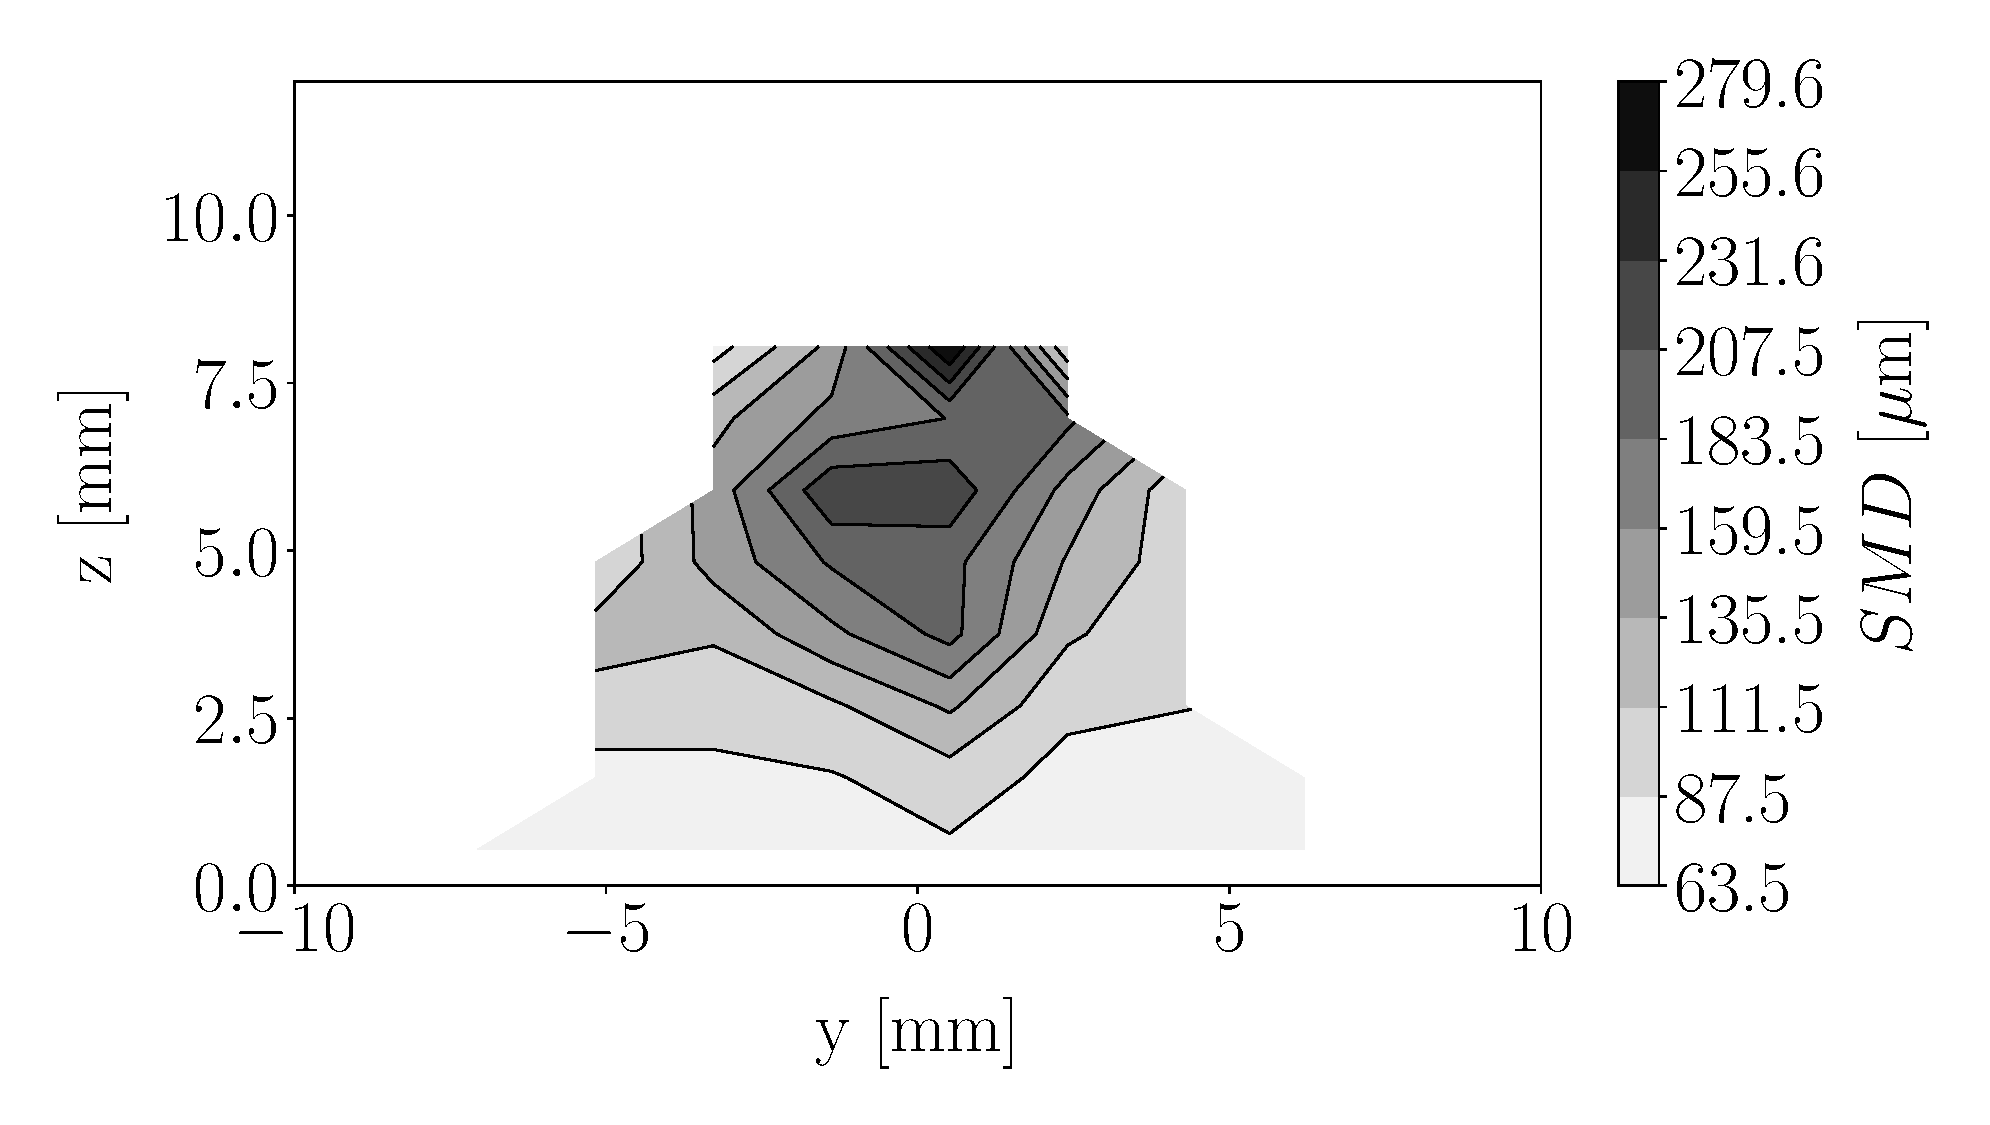
\includegraphics[scale=0.15]{./part2_developments/figures_ch5_resolved_JICF/injectors_SLI/uG75_dx20_x10_SMD_map}
   %\caption{Case UG100\_DX20: crossflow planes}
   %\label{} 
\end{subfigure}
   \hspace{0.17in}
\begin{subfigure}[b]{0.3\textwidth}
	\centering
   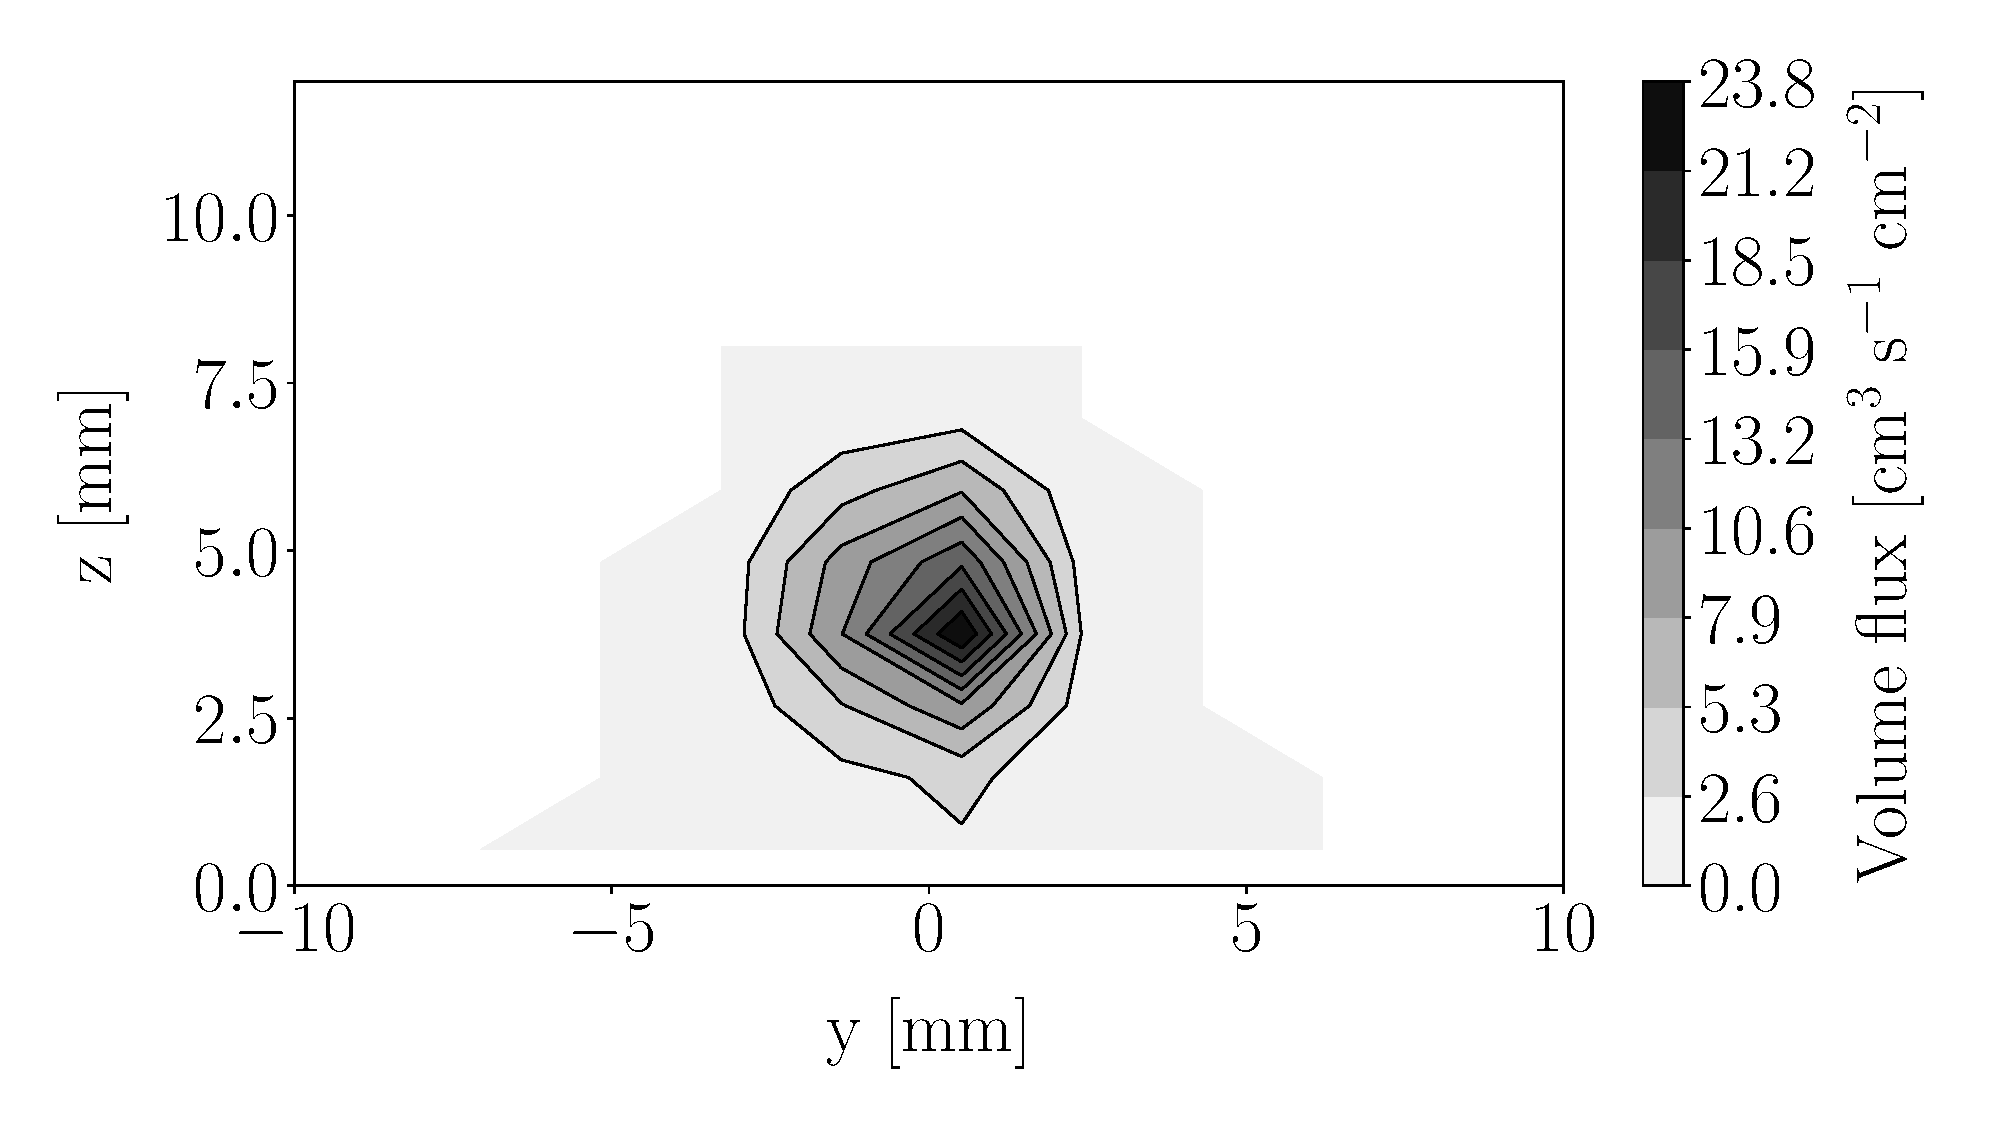
\includegraphics[scale=0.15]{./part2_developments/figures_ch5_resolved_JICF/injectors_SLI/uG75_dx20_x10_volume_flux_map}
   %\caption{Case UG100\_DX20: filming planes}
   %\label{}
\end{subfigure}
   \hspace{0.17in}
\begin{subfigure}[b]{0.3\textwidth}
	\centering
   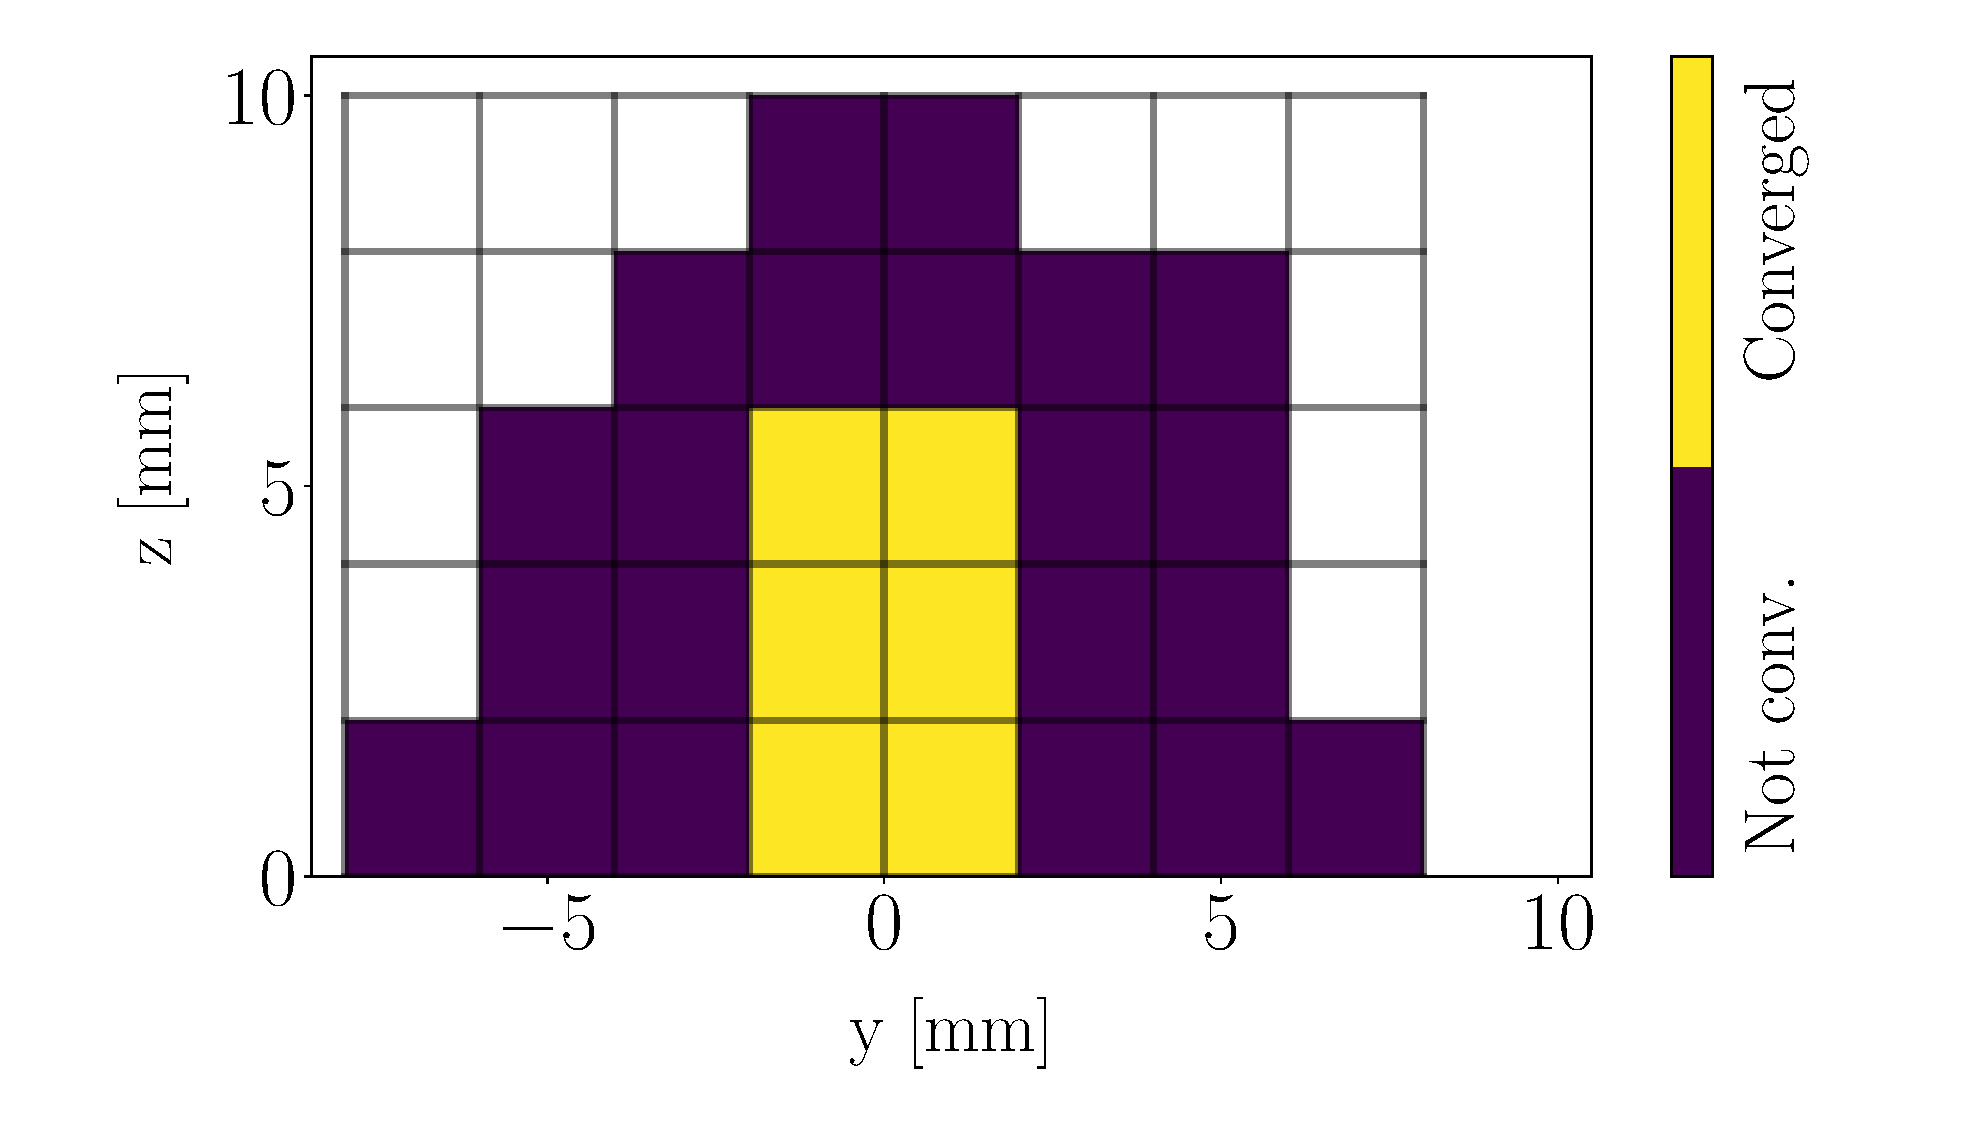
\includegraphics[scale=0.15]{./part2_developments/figures_ch5_resolved_JICF/injectors_SLI/uG75_dx20_x10_convergence_map}
   %\caption{Case UG100\_DX10: crossflow planes}
   %\label{} 
\end{subfigure}

\vskip\baselineskip

\begin{subfigure}[b]{0.3\textwidth}
	\centering
   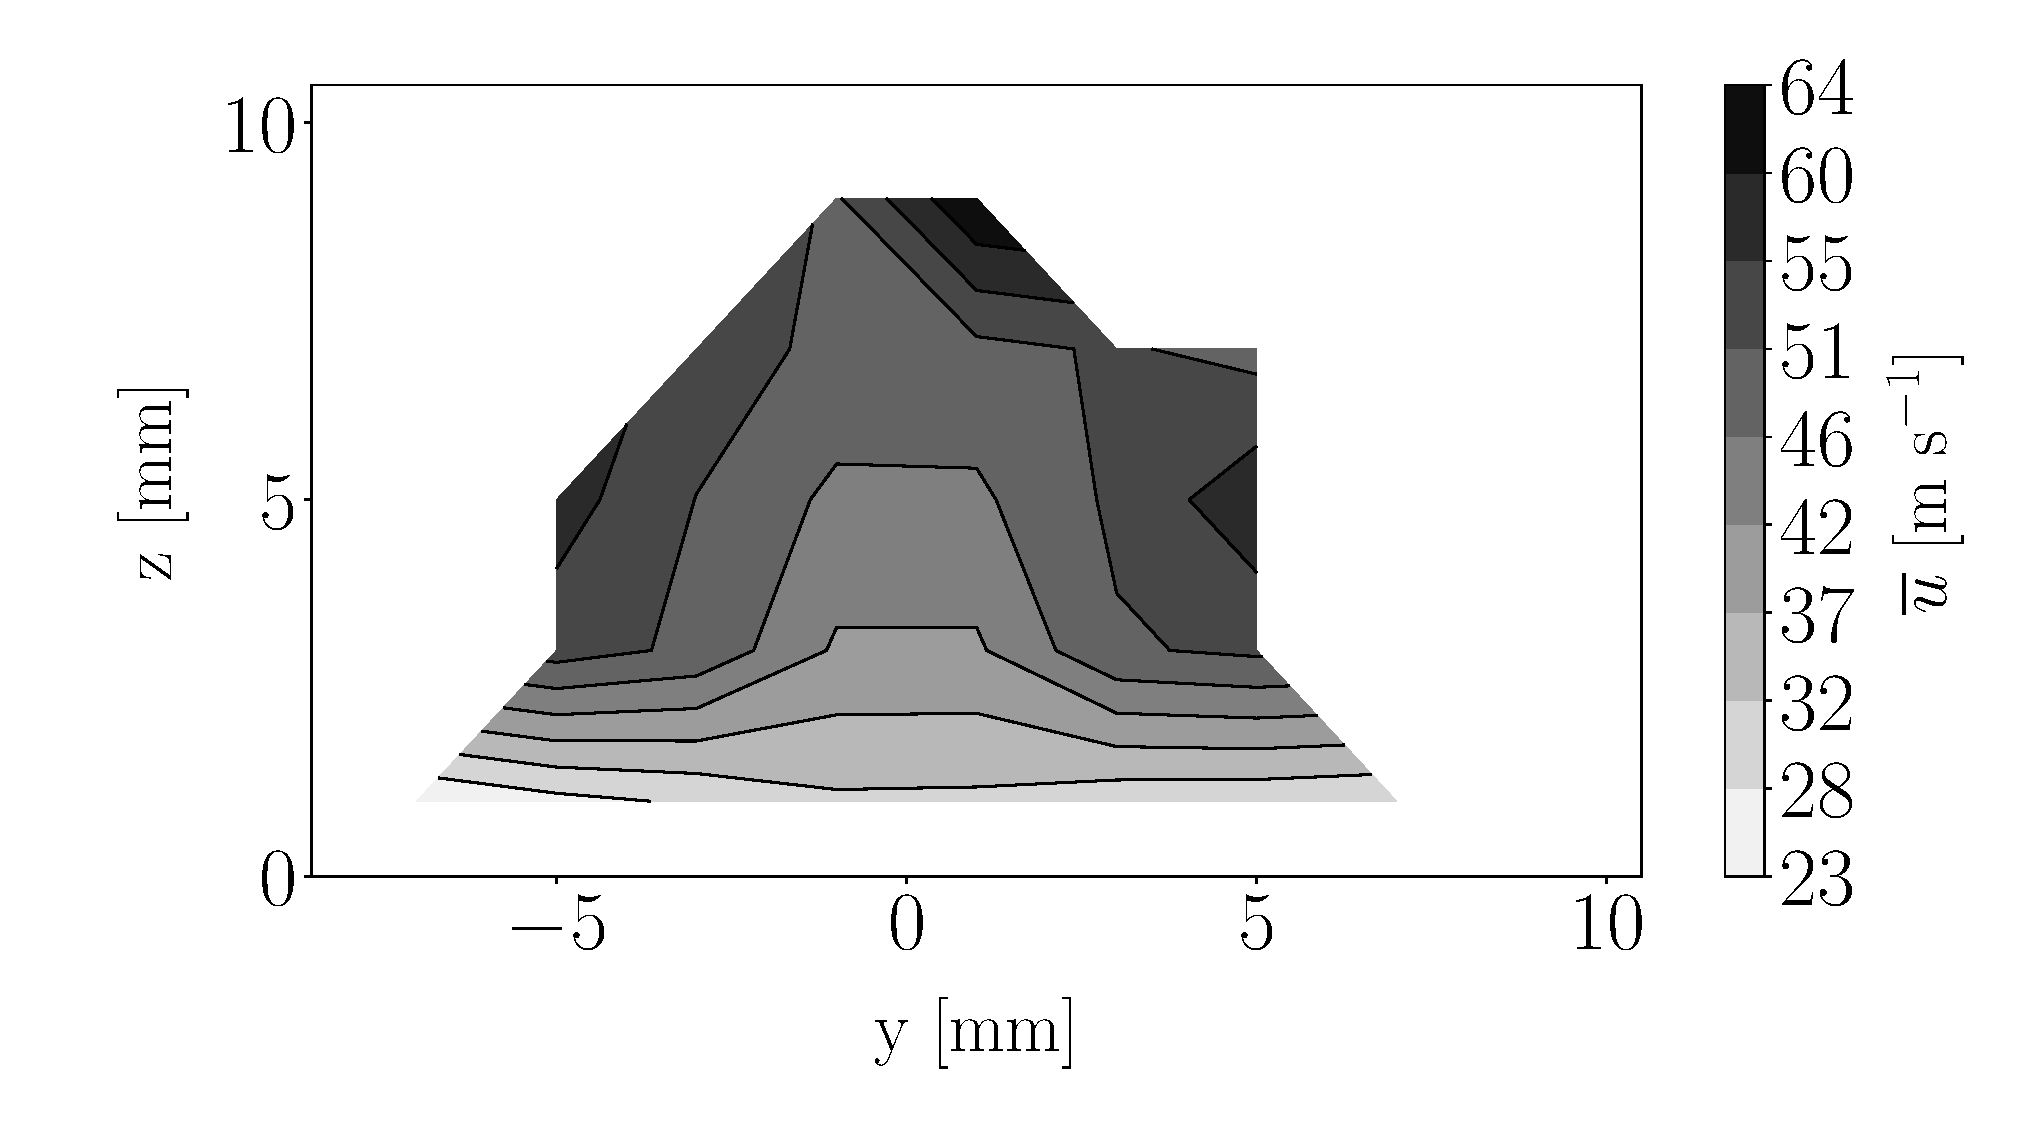
\includegraphics[scale=0.15]{./part2_developments/figures_ch5_resolved_JICF/injectors_SLI/uG75_dx20_x10_ux_mean_map}
   %\caption{Case UG100\_DX20: crossflow planes}
   %\label{} 
\end{subfigure}
   \hspace{0.17in}
\begin{subfigure}[b]{0.3\textwidth}
	\centering
   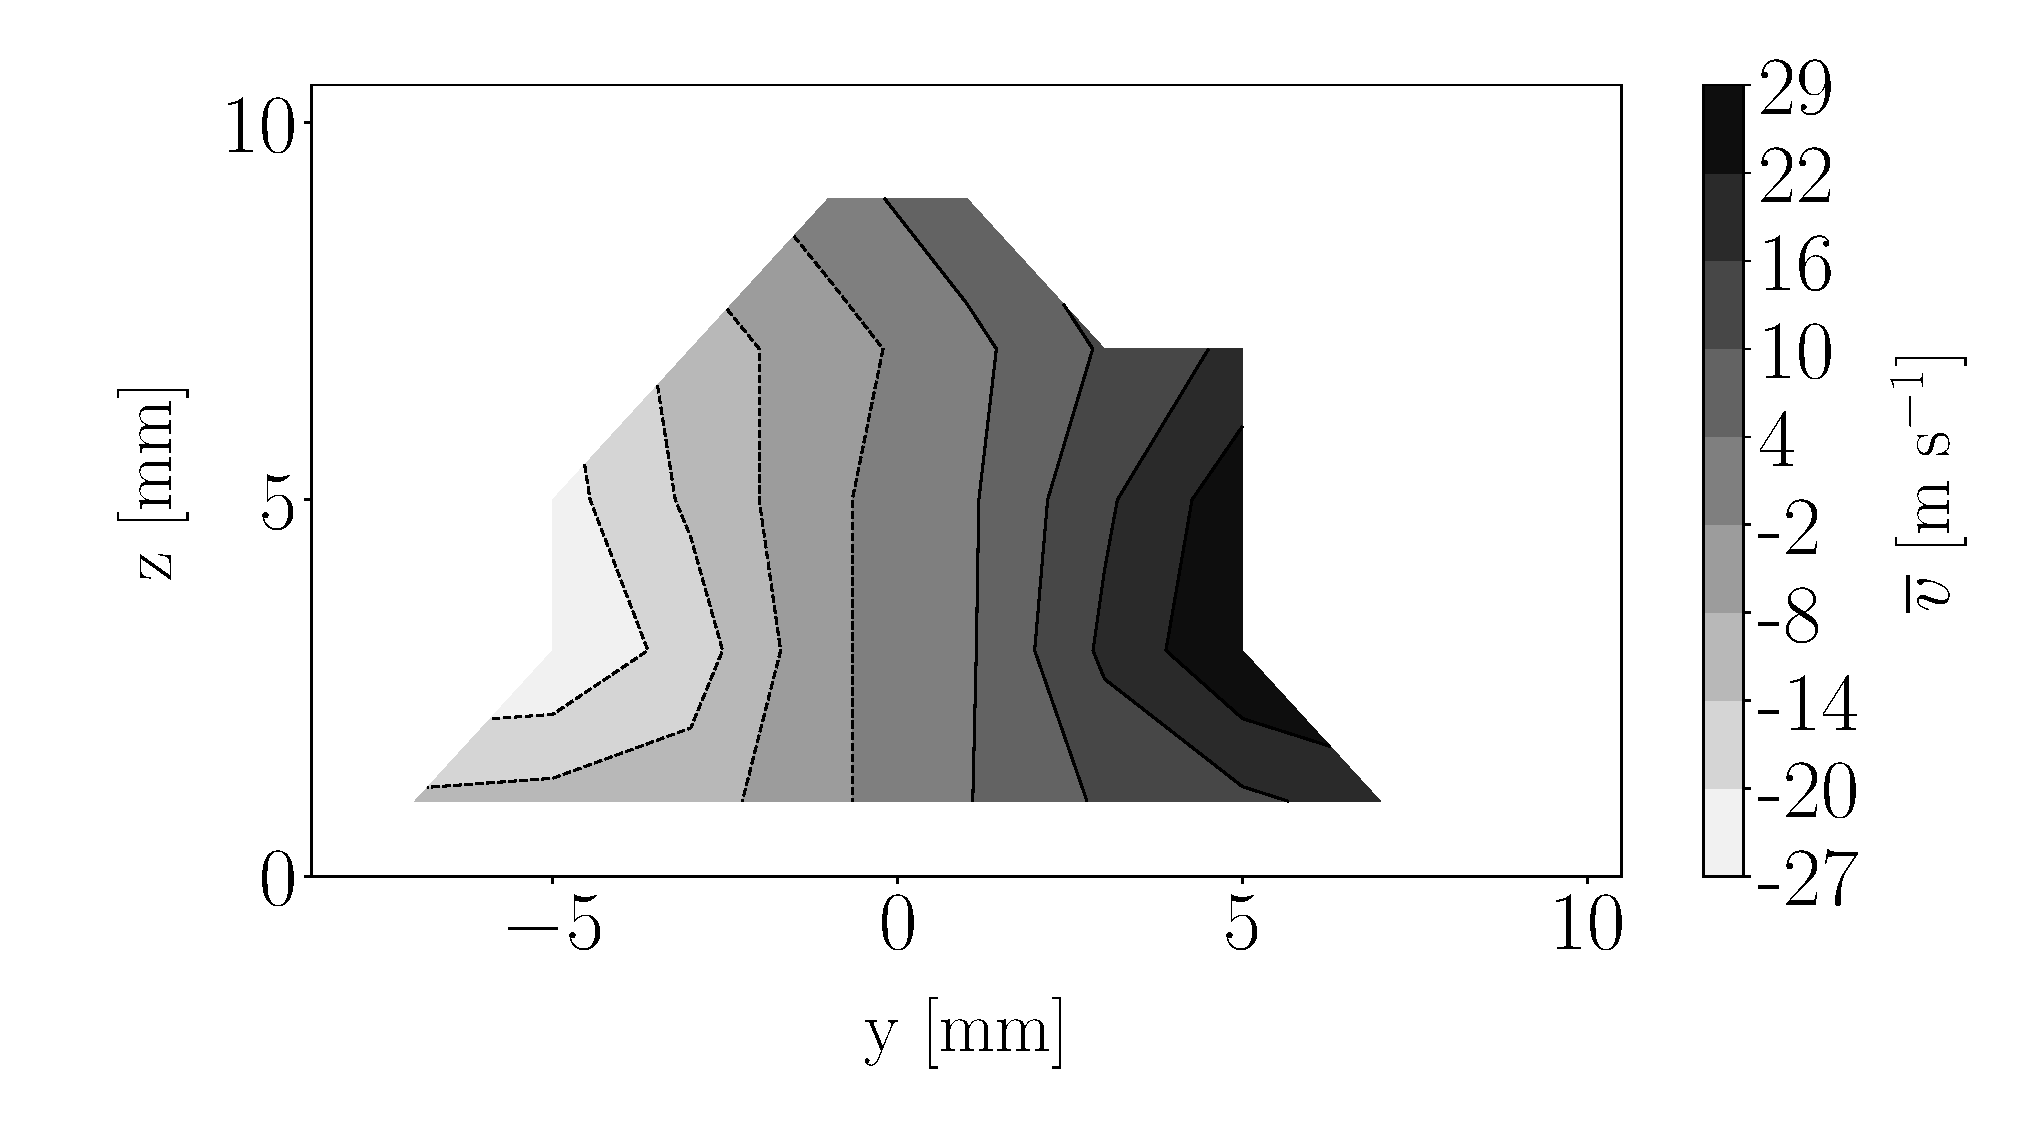
\includegraphics[scale=0.15]{./part2_developments/figures_ch5_resolved_JICF/injectors_SLI/uG75_dx20_x10_uy_mean_map}
   %\caption{Case UG100\_DX20: filming planes}
   %\label{}
\end{subfigure}
   \hspace{0.17in}
\begin{subfigure}[b]{0.3\textwidth}
	\centering
   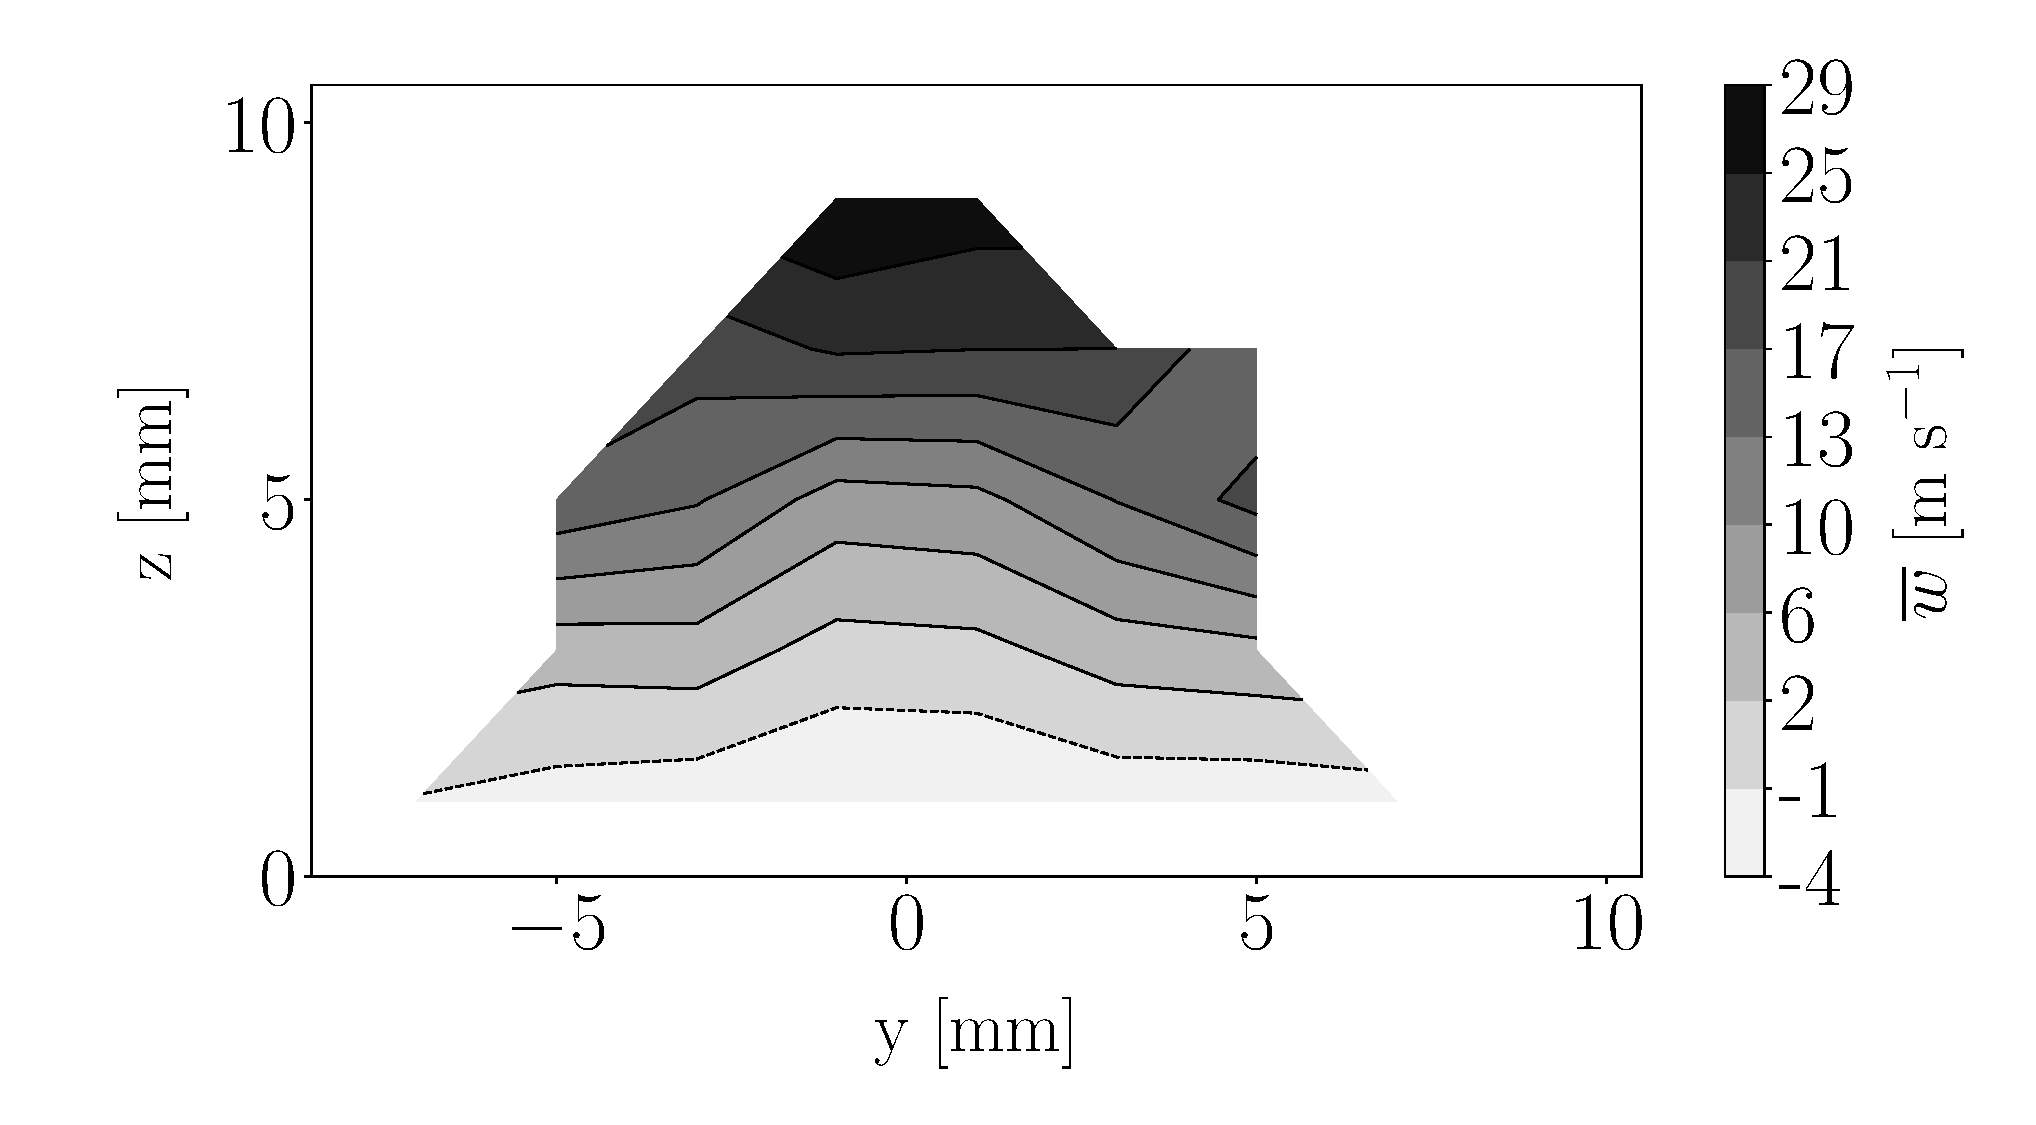
\includegraphics[scale=0.15]{./part2_developments/figures_ch5_resolved_JICF/injectors_SLI/uG75_dx20_x10_uz_mean_map}
   %\caption{Case UG100\_DX10: crossflow planes}
   %\label{} 
\end{subfigure}
\caption{Spray states at x = 10 mm for case UG75\_DX20}
\label{fig:injectors_sli_uG75_dx20_x10}
\end{figure}


%%%%%%%%%%%%%%%% UG75_DX10, x = 15 mm


\begin{figure}[h!]
\centering
\begin{subfigure}[b]{0.3\textwidth}
	\centering
   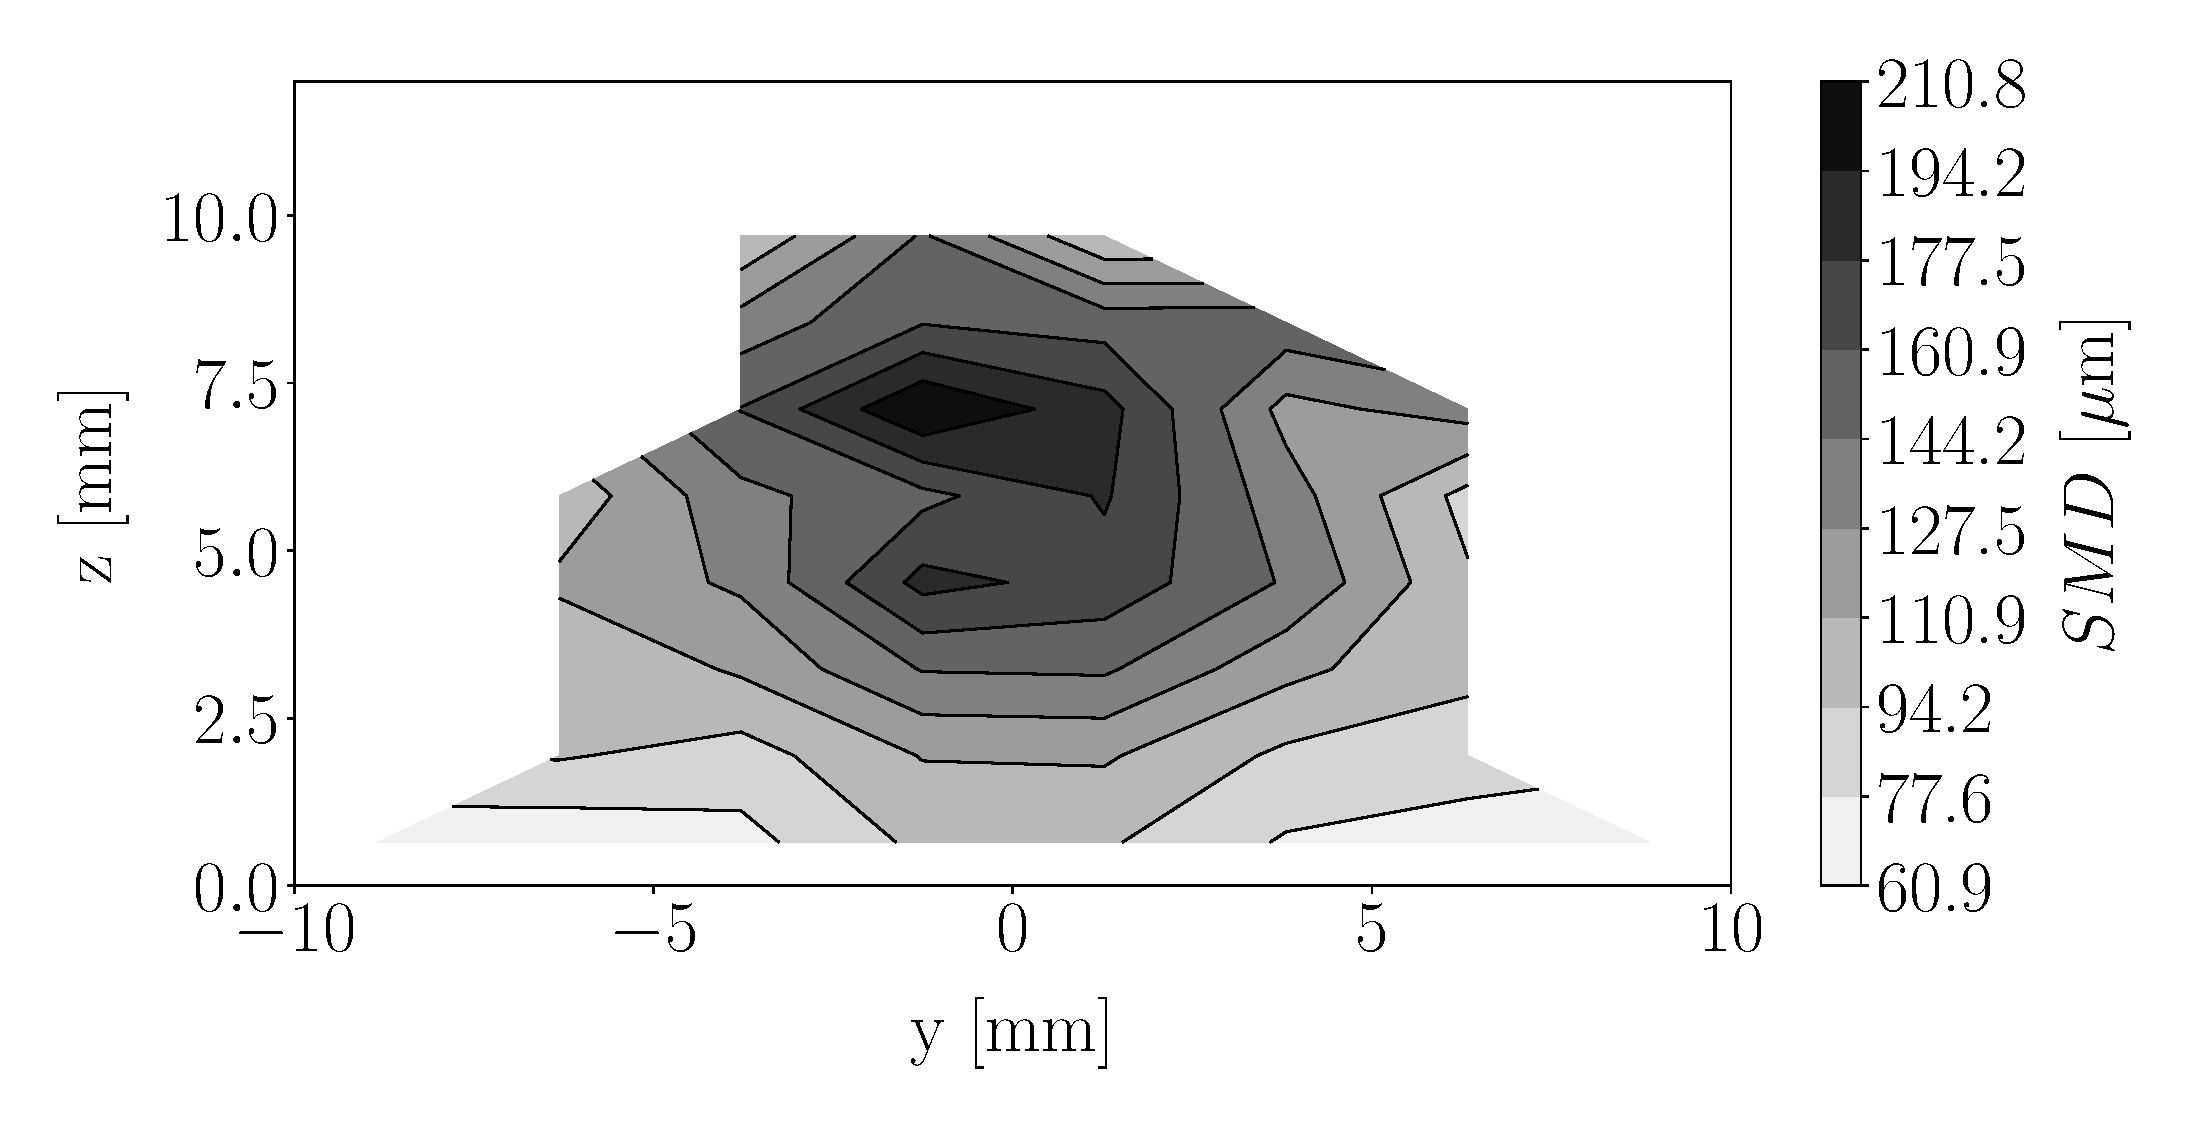
\includegraphics[scale=\scaleSLIJICF]{./part2_developments/figures_ch5_resolved_JICF/injectors_SLI/uG75_dx20_x15_SMD_map}
   %\caption{Case UG100\_DX20: crossflow planes}
   %\label{} 
\end{subfigure}
   \hspace{0.17in}
\begin{subfigure}[b]{0.3\textwidth}
	\centering
   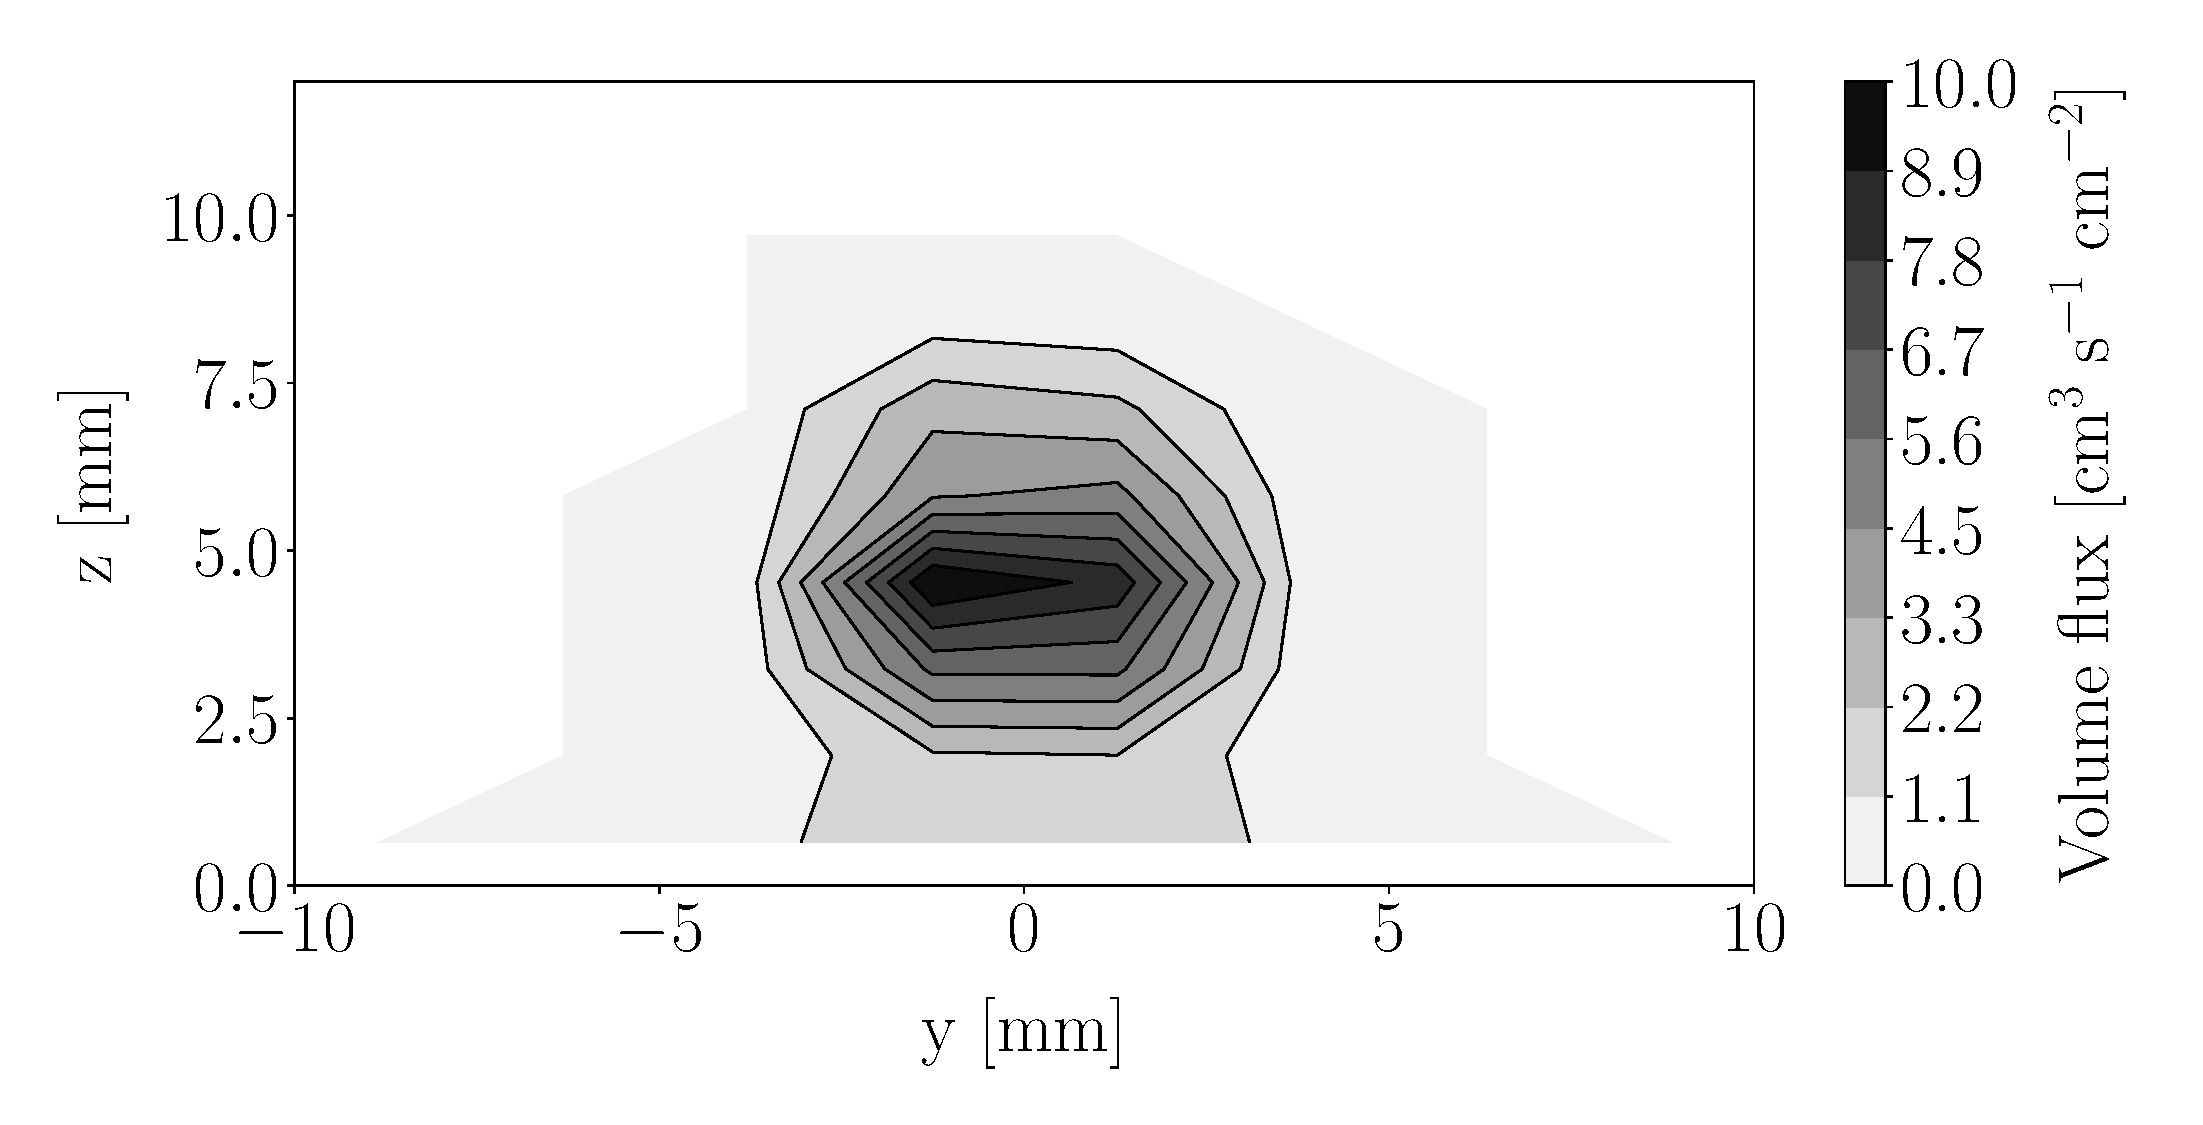
\includegraphics[scale=\scaleSLIJICF]{./part2_developments/figures_ch5_resolved_JICF/injectors_SLI/uG75_dx20_x15_volume_flux_map}
   %\caption{Case UG100\_DX20: filming planes}
   %\label{}
\end{subfigure}
   \hspace{0.17in}
\begin{subfigure}[b]{0.3\textwidth}
	\centering
   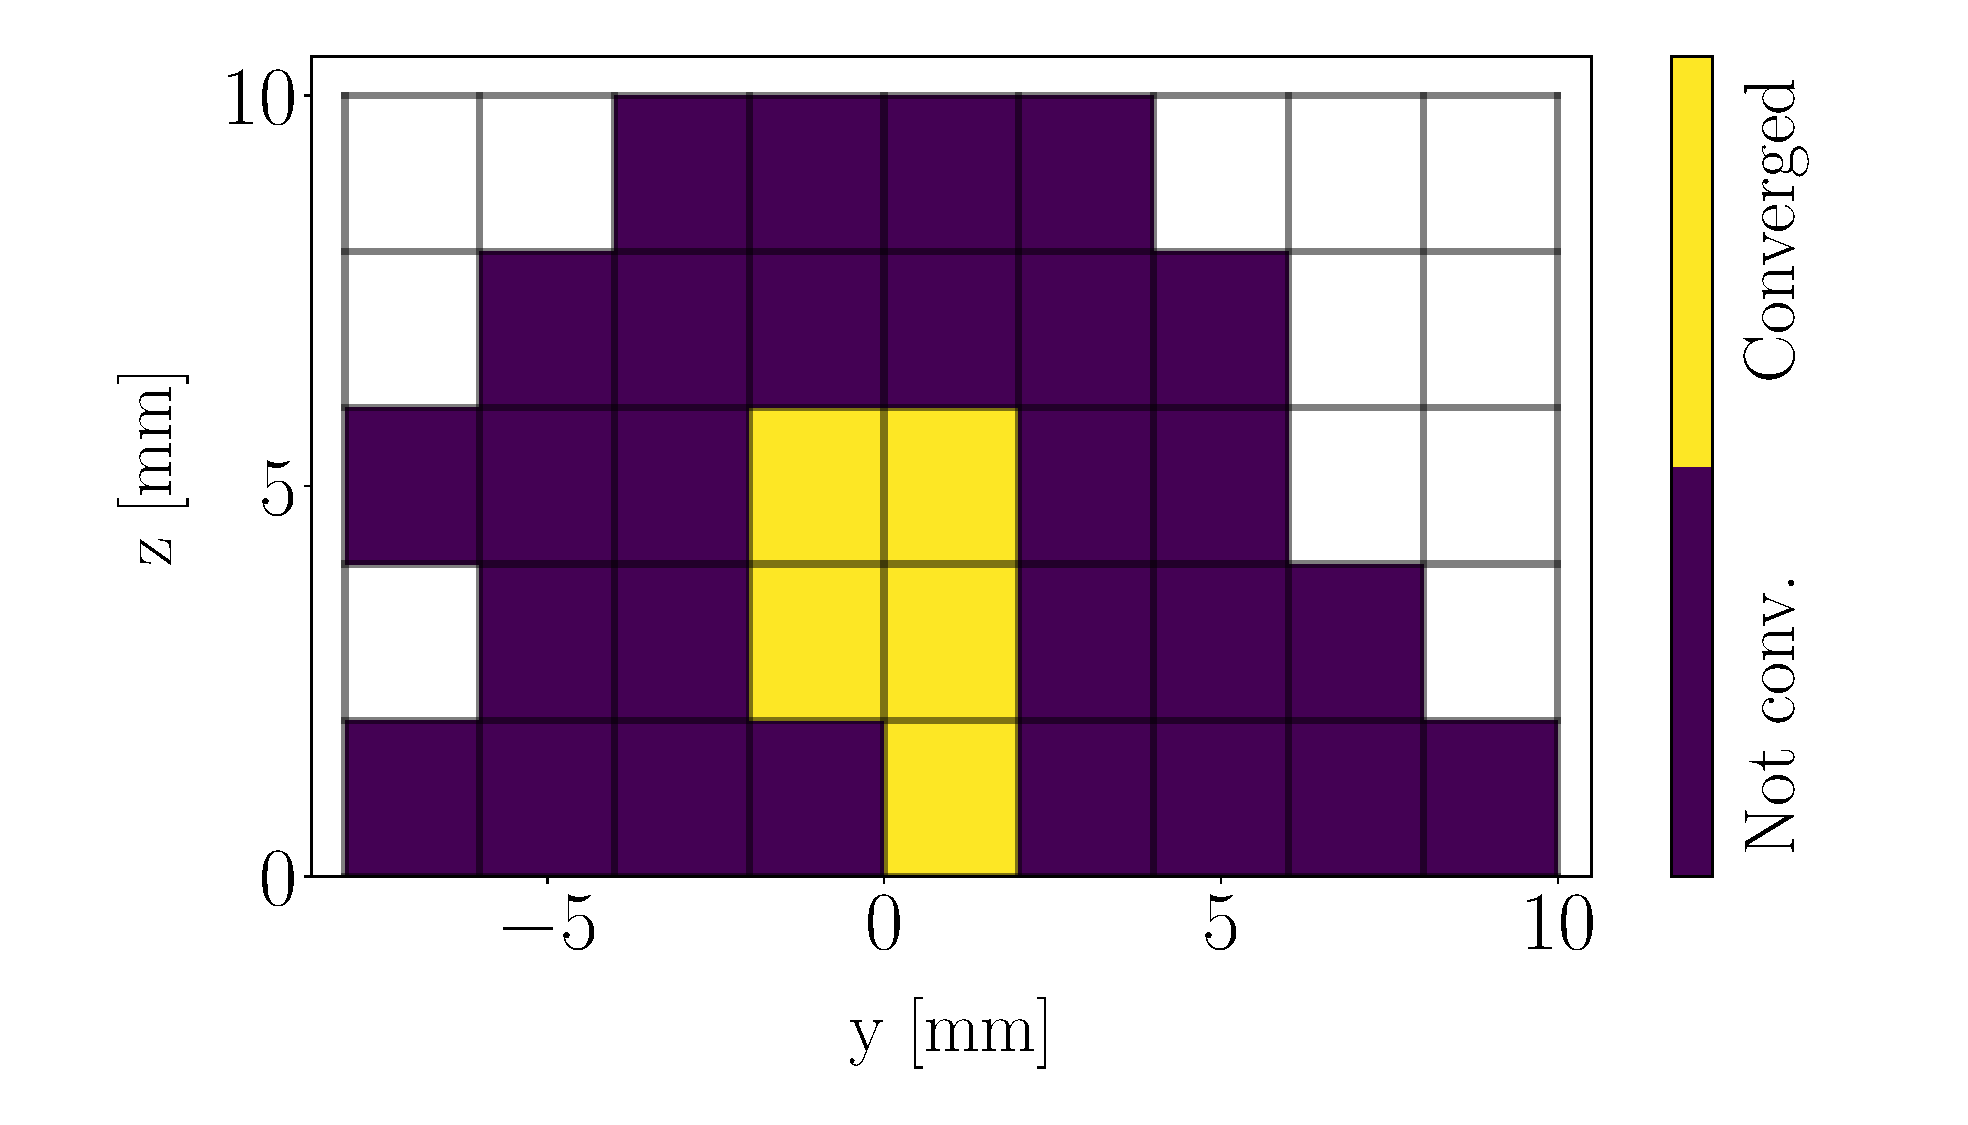
\includegraphics[scale=\scaleSLIJICF]{./part2_developments/figures_ch5_resolved_JICF/injectors_SLI/uG75_dx20_x15_convergence_map}
   %\caption{Case UG100\_DX10: crossflow planes}
   %\label{} 
\end{subfigure}

\vskip\baselineskip

\begin{subfigure}[b]{0.3\textwidth}
	\centering
   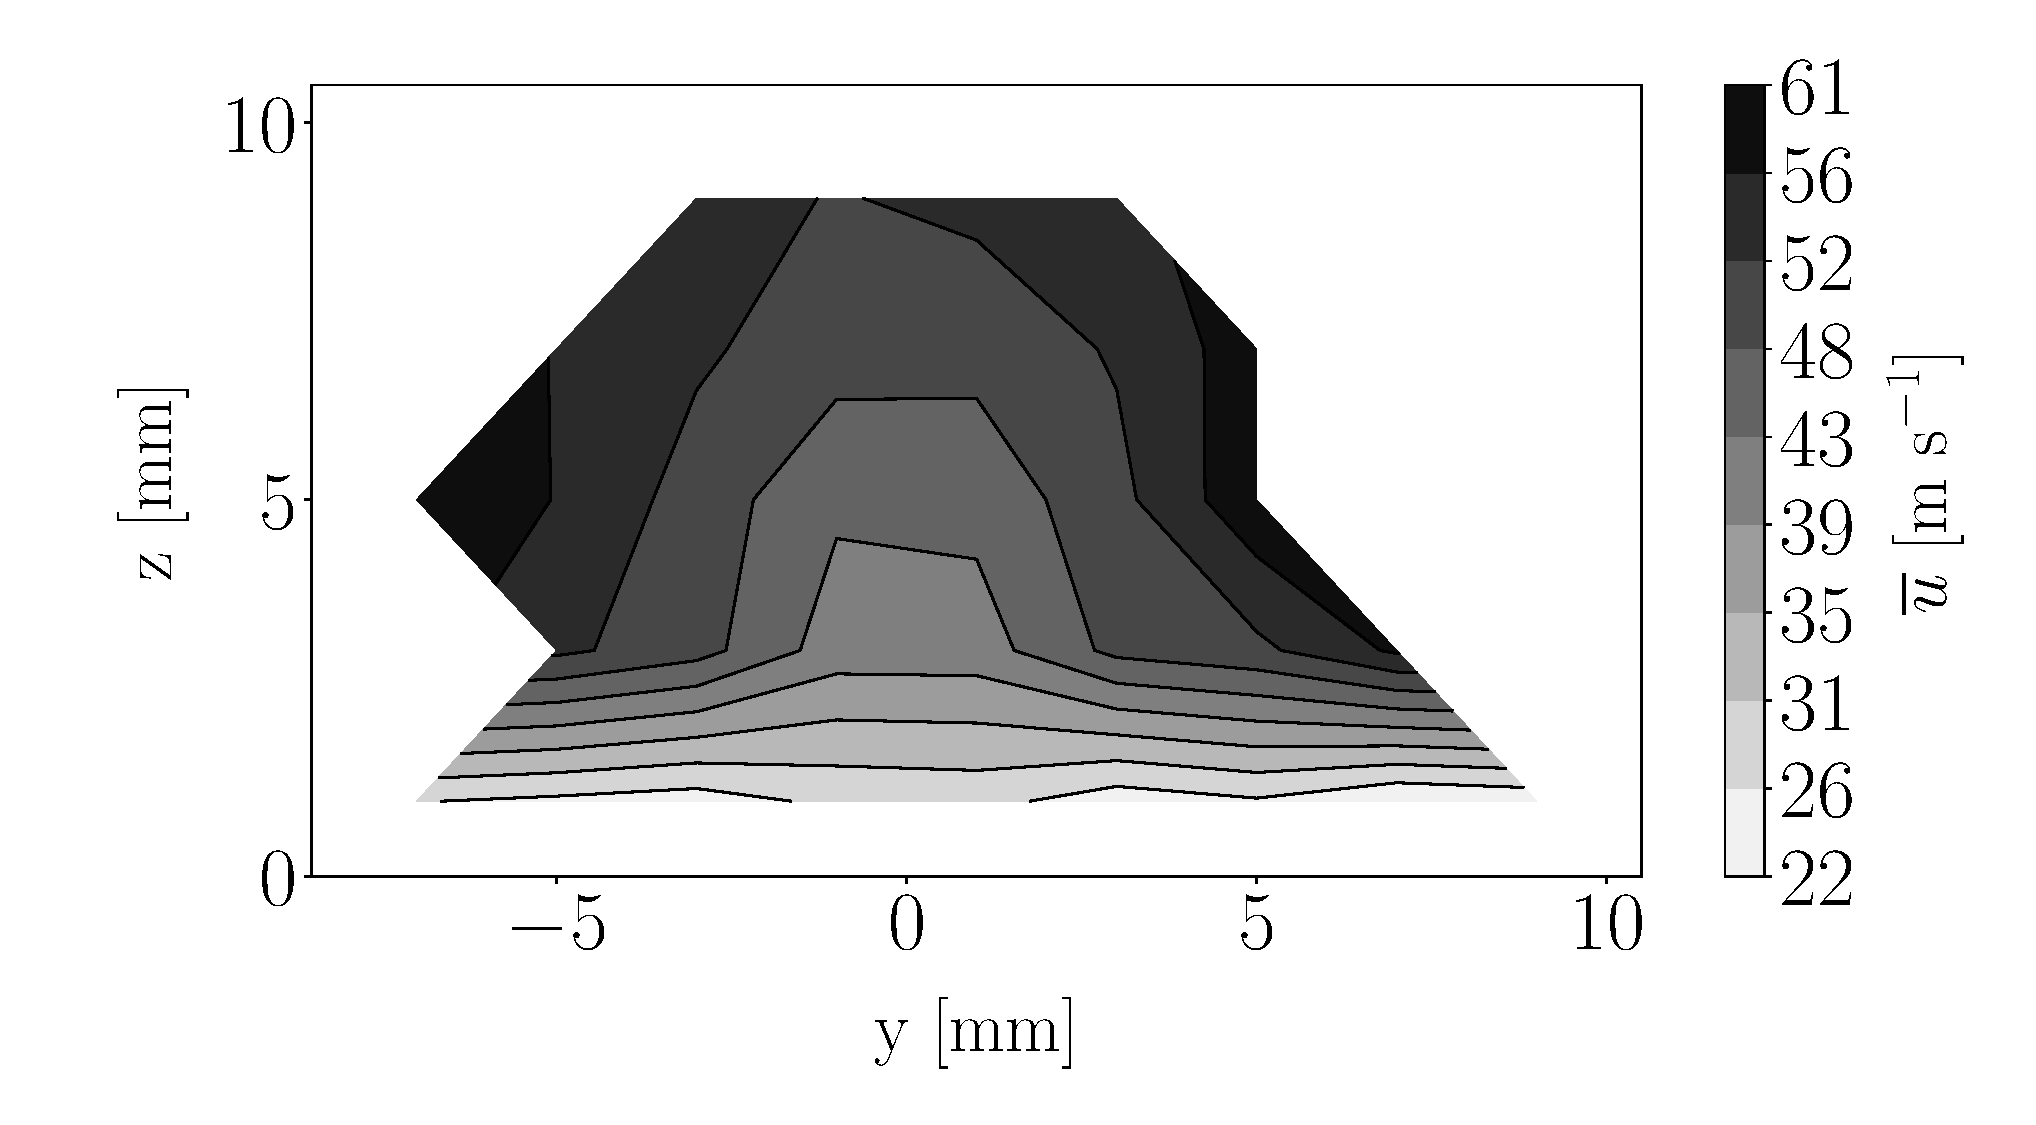
\includegraphics[scale=\scaleSLIJICF]{./part2_developments/figures_ch5_resolved_JICF/injectors_SLI/uG75_dx20_x15_ux_mean_map}
   %\caption{Case UG100\_DX20: crossflow planes}
   %\label{} 
\end{subfigure}
   \hspace{0.17in}
\begin{subfigure}[b]{0.3\textwidth}
	\centering
   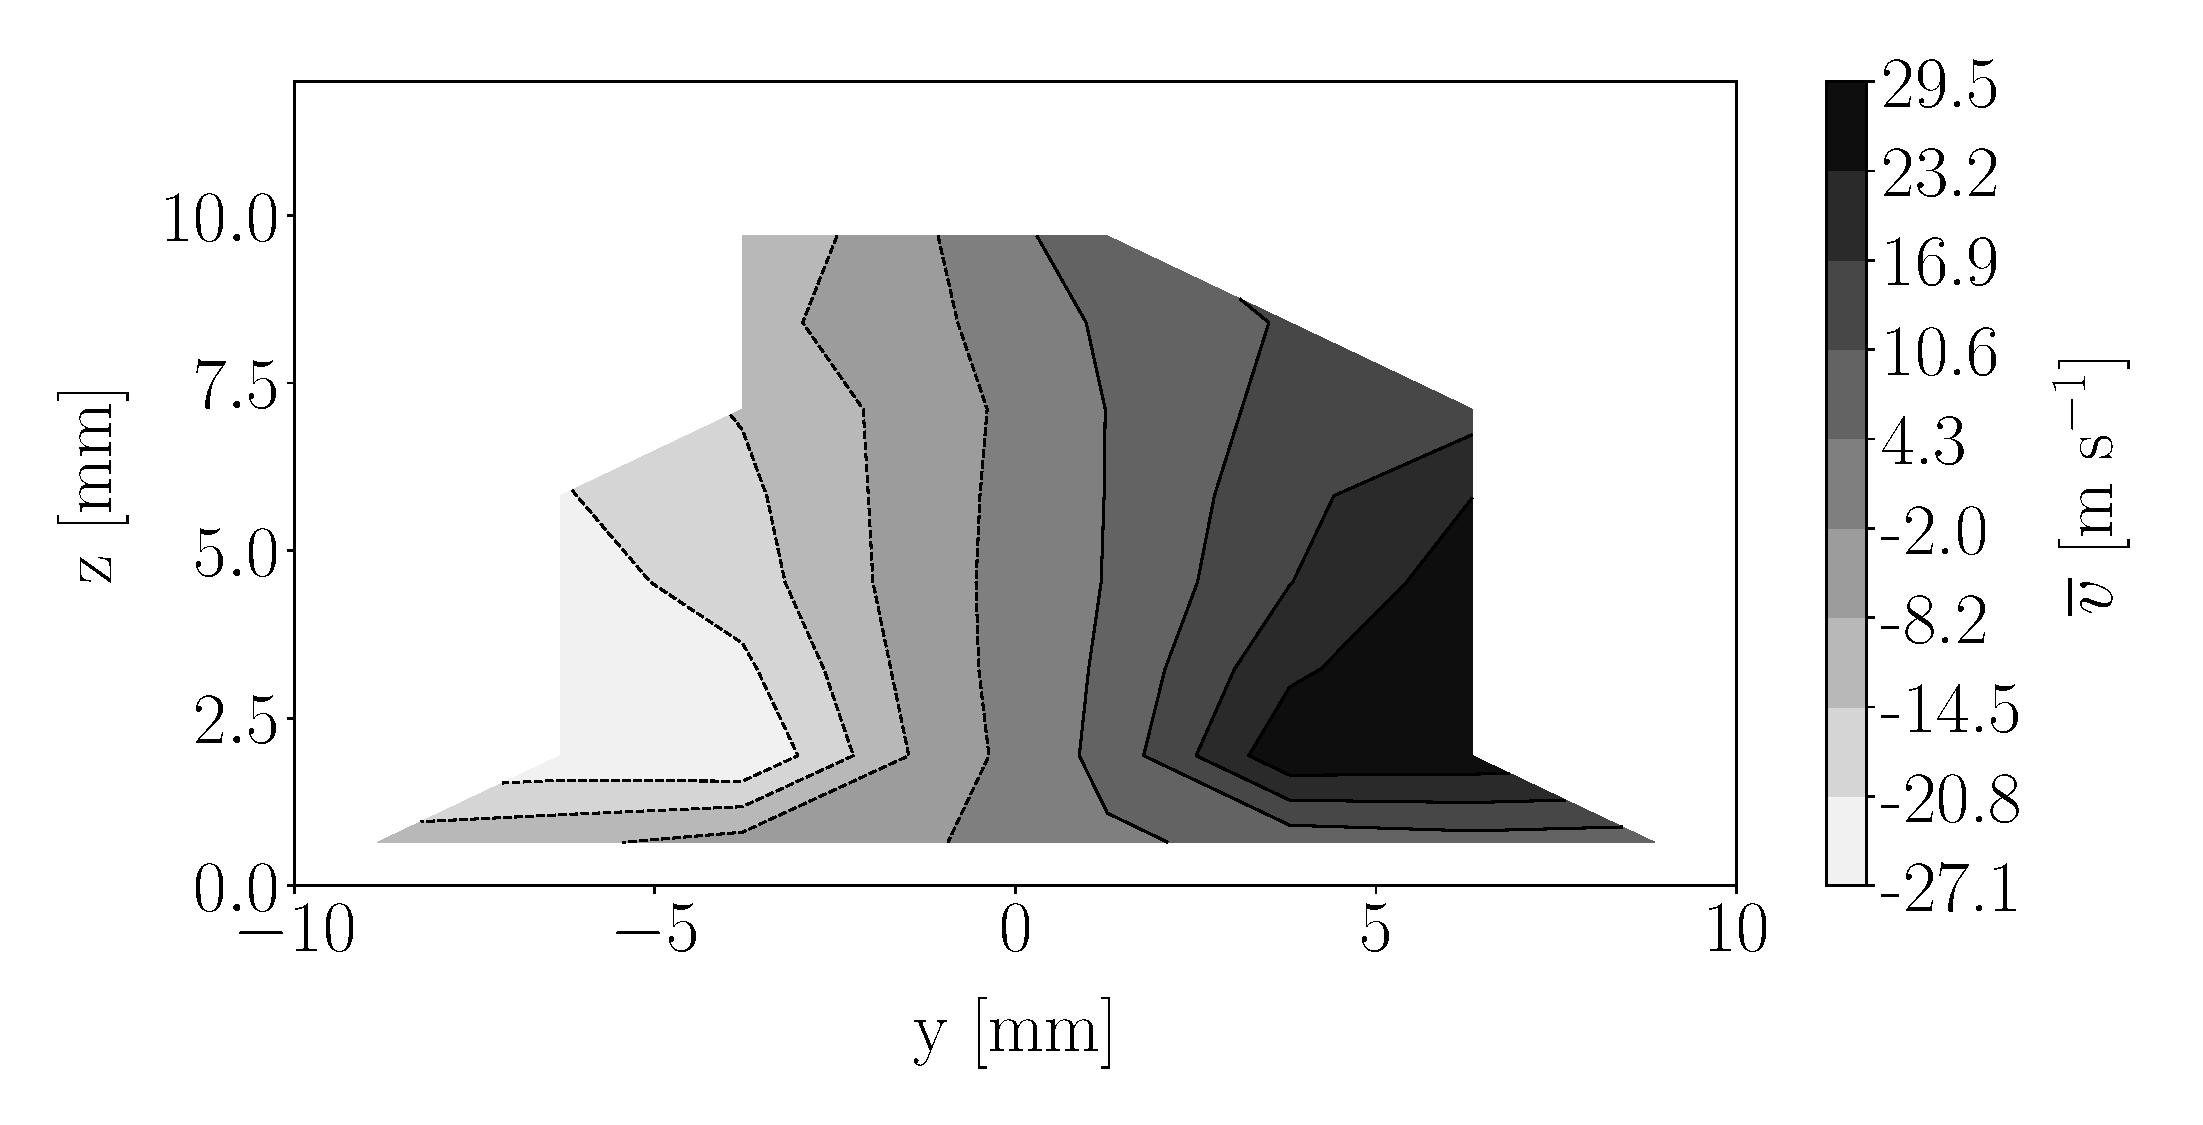
\includegraphics[scale=\scaleSLIJICF]{./part2_developments/figures_ch5_resolved_JICF/injectors_SLI/uG75_dx20_x15_uy_mean_map}
   %\caption{Case UG100\_DX20: filming planes}
   %\label{}
\end{subfigure}
   \hspace{0.17in}
\begin{subfigure}[b]{0.3\textwidth}
	\centering
   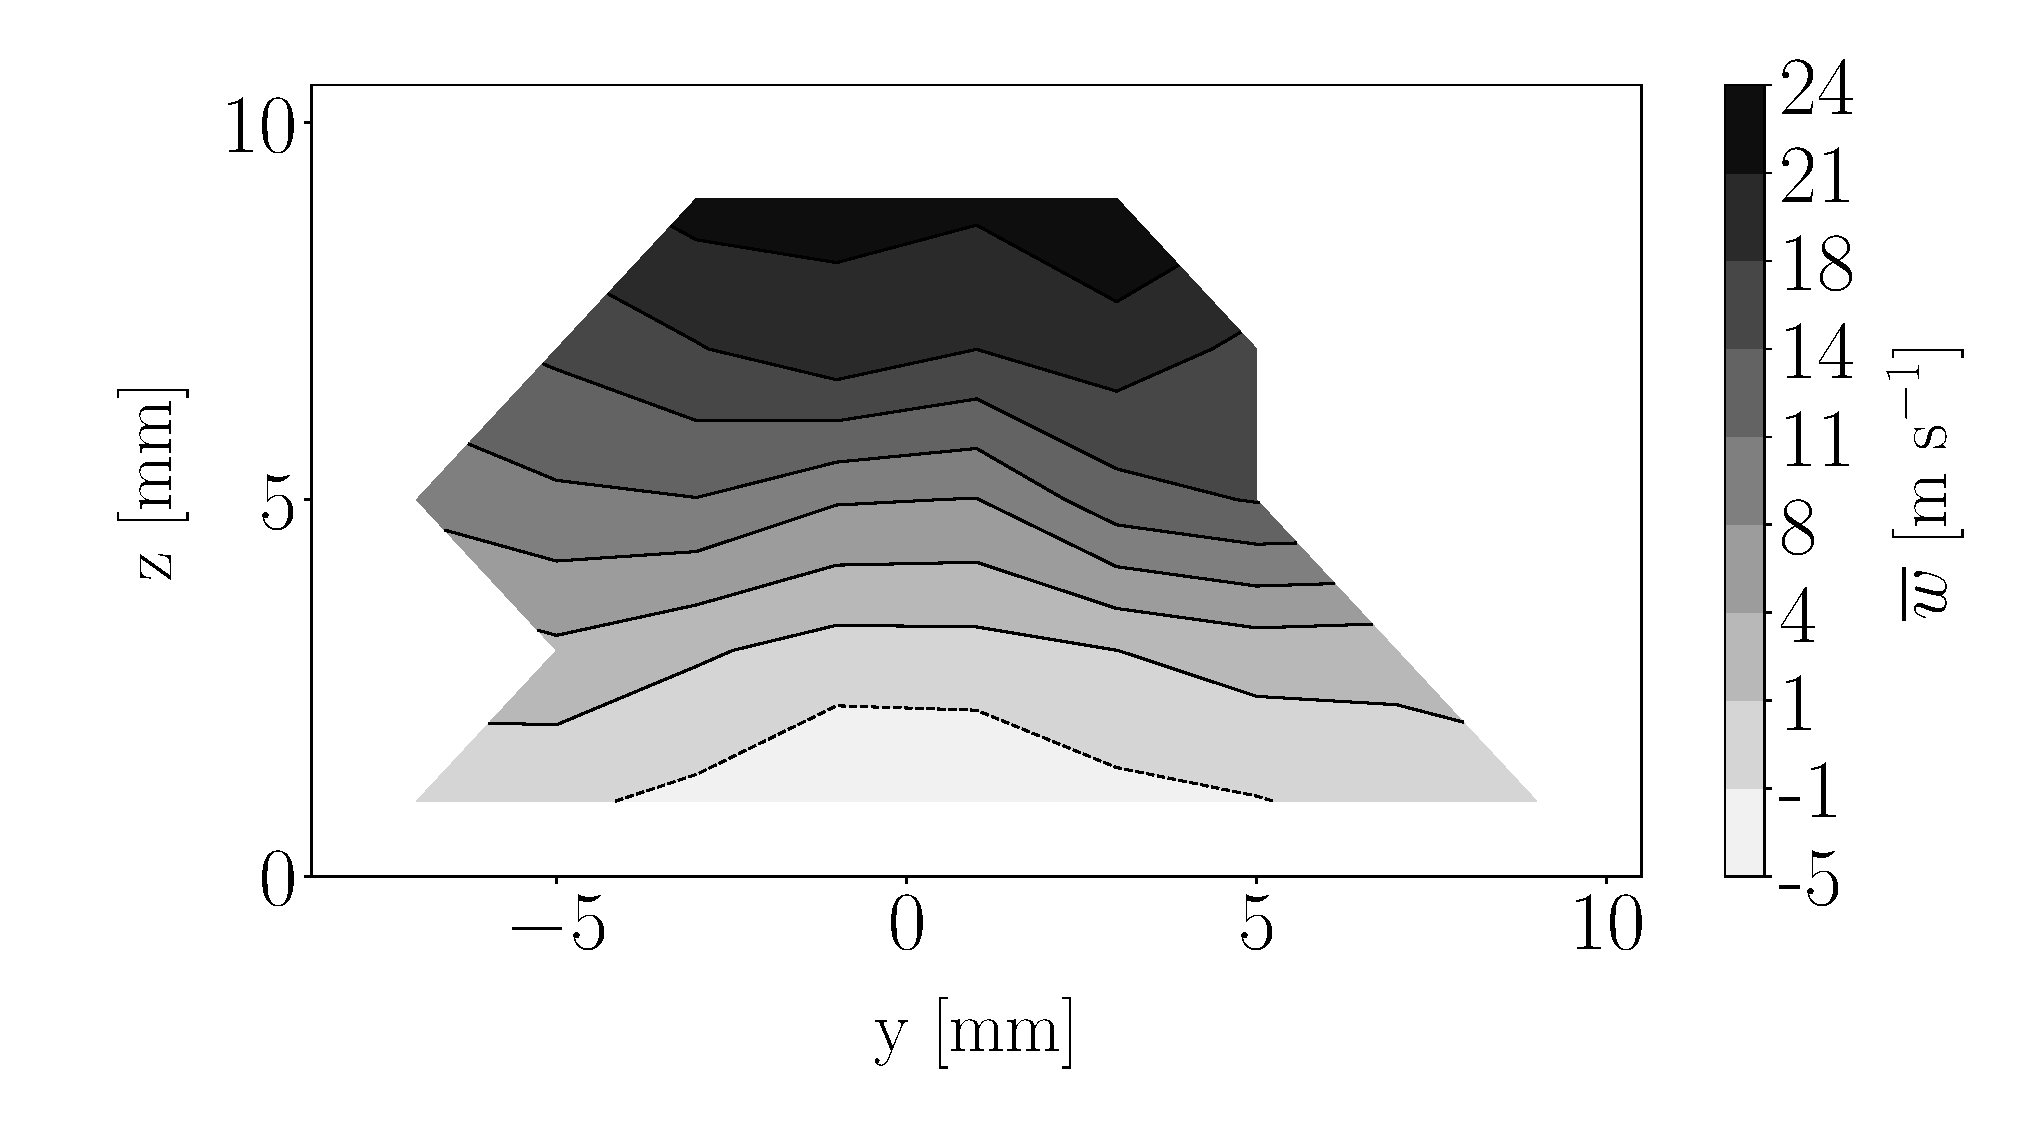
\includegraphics[scale=\scaleSLIJICF]{./part2_developments/figures_ch5_resolved_JICF/injectors_SLI/uG75_dx20_x15_uz_mean_map}
   %\caption{Case UG100\_DX10: crossflow planes}
   %\label{} 
\end{subfigure}
\caption{Spray states at x = 15 mm for case UG75\_DX20}
\label{fig:injectors_sli_uG75_dx20_x15}
\end{figure}


\clearpage

\subsubsection*{Case UG100\_DX10}



%%%%%%%%%%%%%%%% UG100_DX10, x = 5 mm


\begin{figure}[h!]
\centering
\begin{subfigure}[b]{0.3\textwidth}
	\centering
   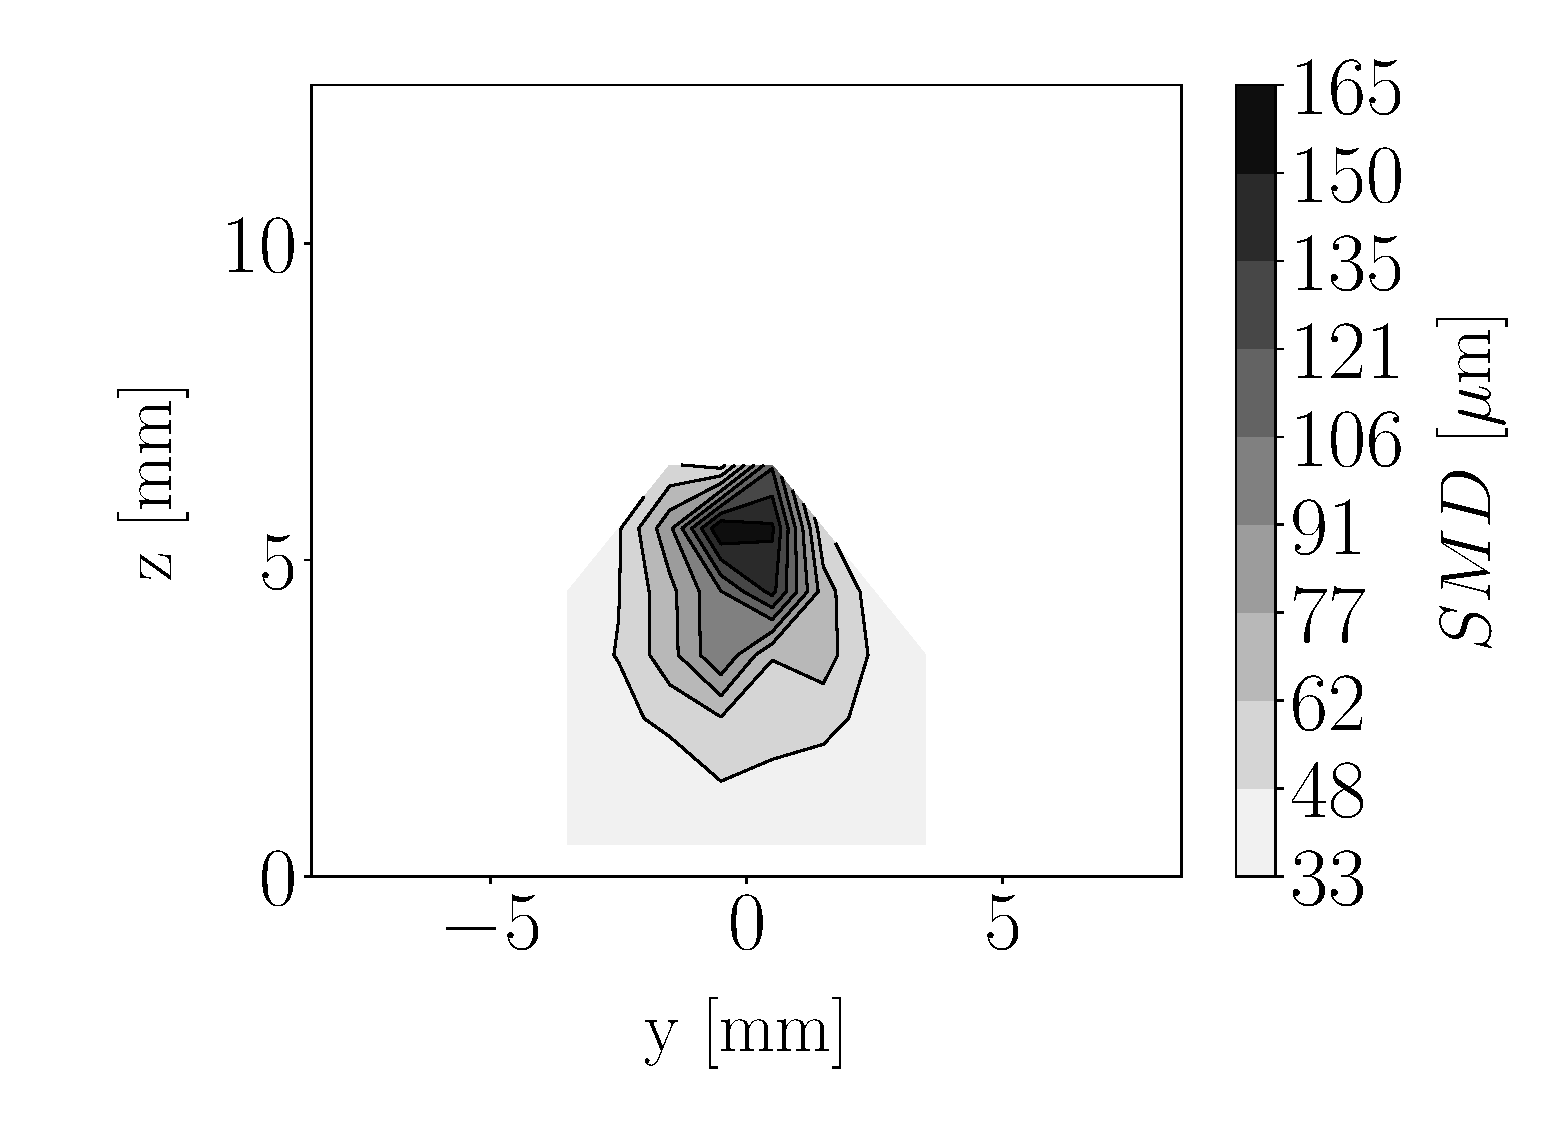
\includegraphics[scale=\scaleSLIJICF]{./part2_developments/figures_ch5_resolved_JICF/injectors_SLI/uG100_dx10_x05_SMD_map}
   %\caption{Case UG100\_DX20: crossflow planes}
   %\label{} 
\end{subfigure}
   \hspace{0.17in}
\begin{subfigure}[b]{0.3\textwidth}
	\centering
   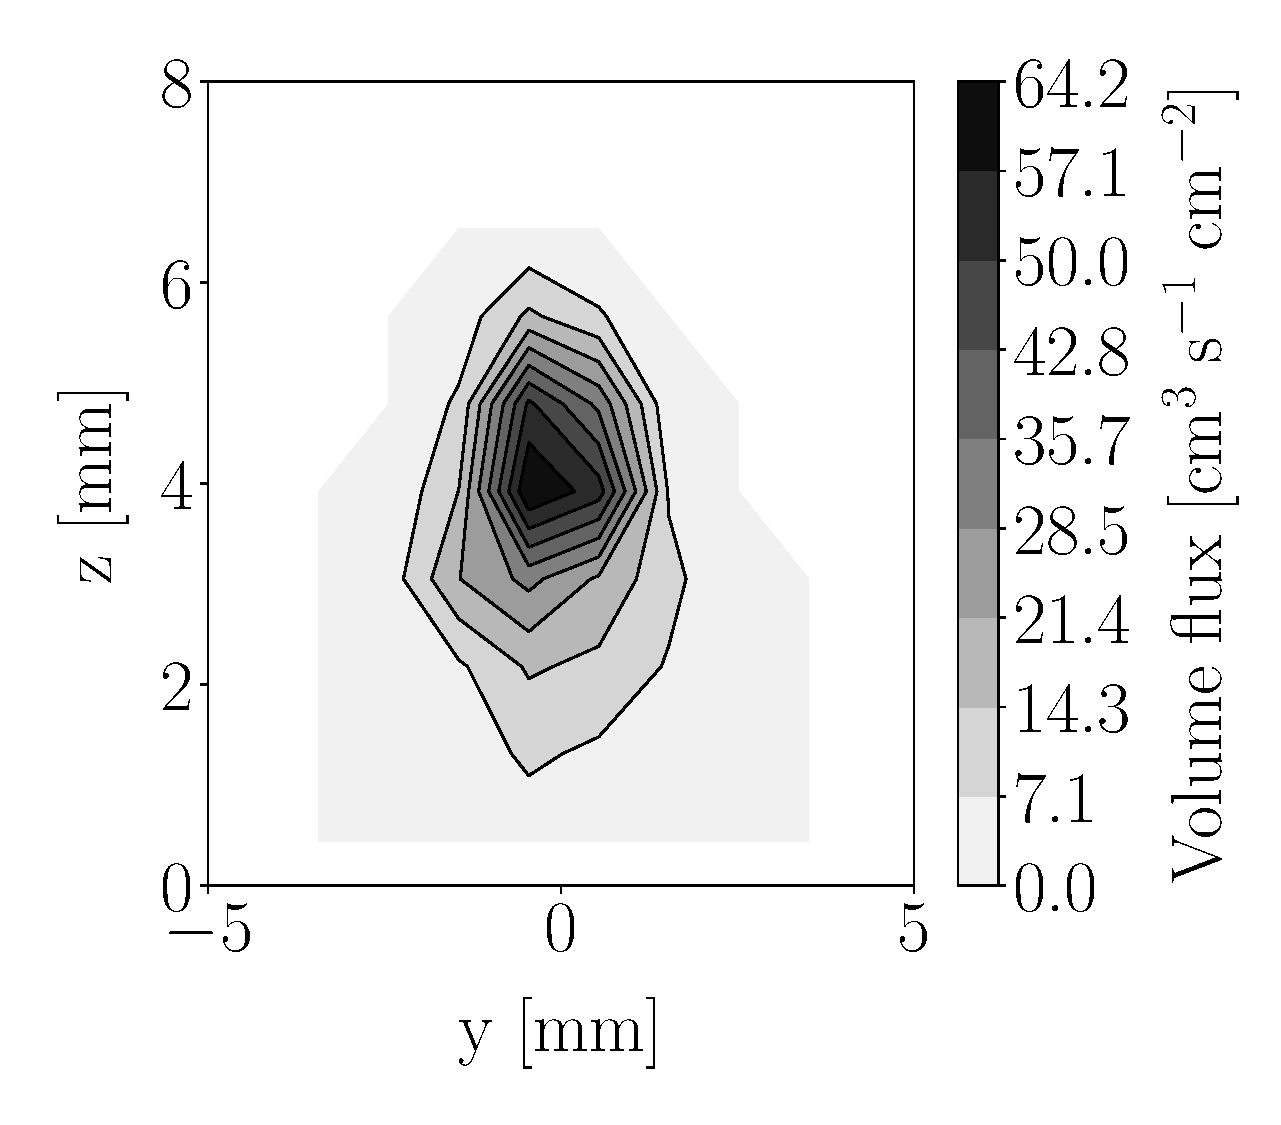
\includegraphics[scale=\scaleSLIJICF]{./part2_developments/figures_ch5_resolved_JICF/injectors_SLI/uG100_dx10_x05_volume_flux_map}
   %\caption{Case UG100\_DX20: filming planes}
   %\label{}
\end{subfigure}
   \hspace{0.17in}
\begin{subfigure}[b]{0.3\textwidth}
	\centering
   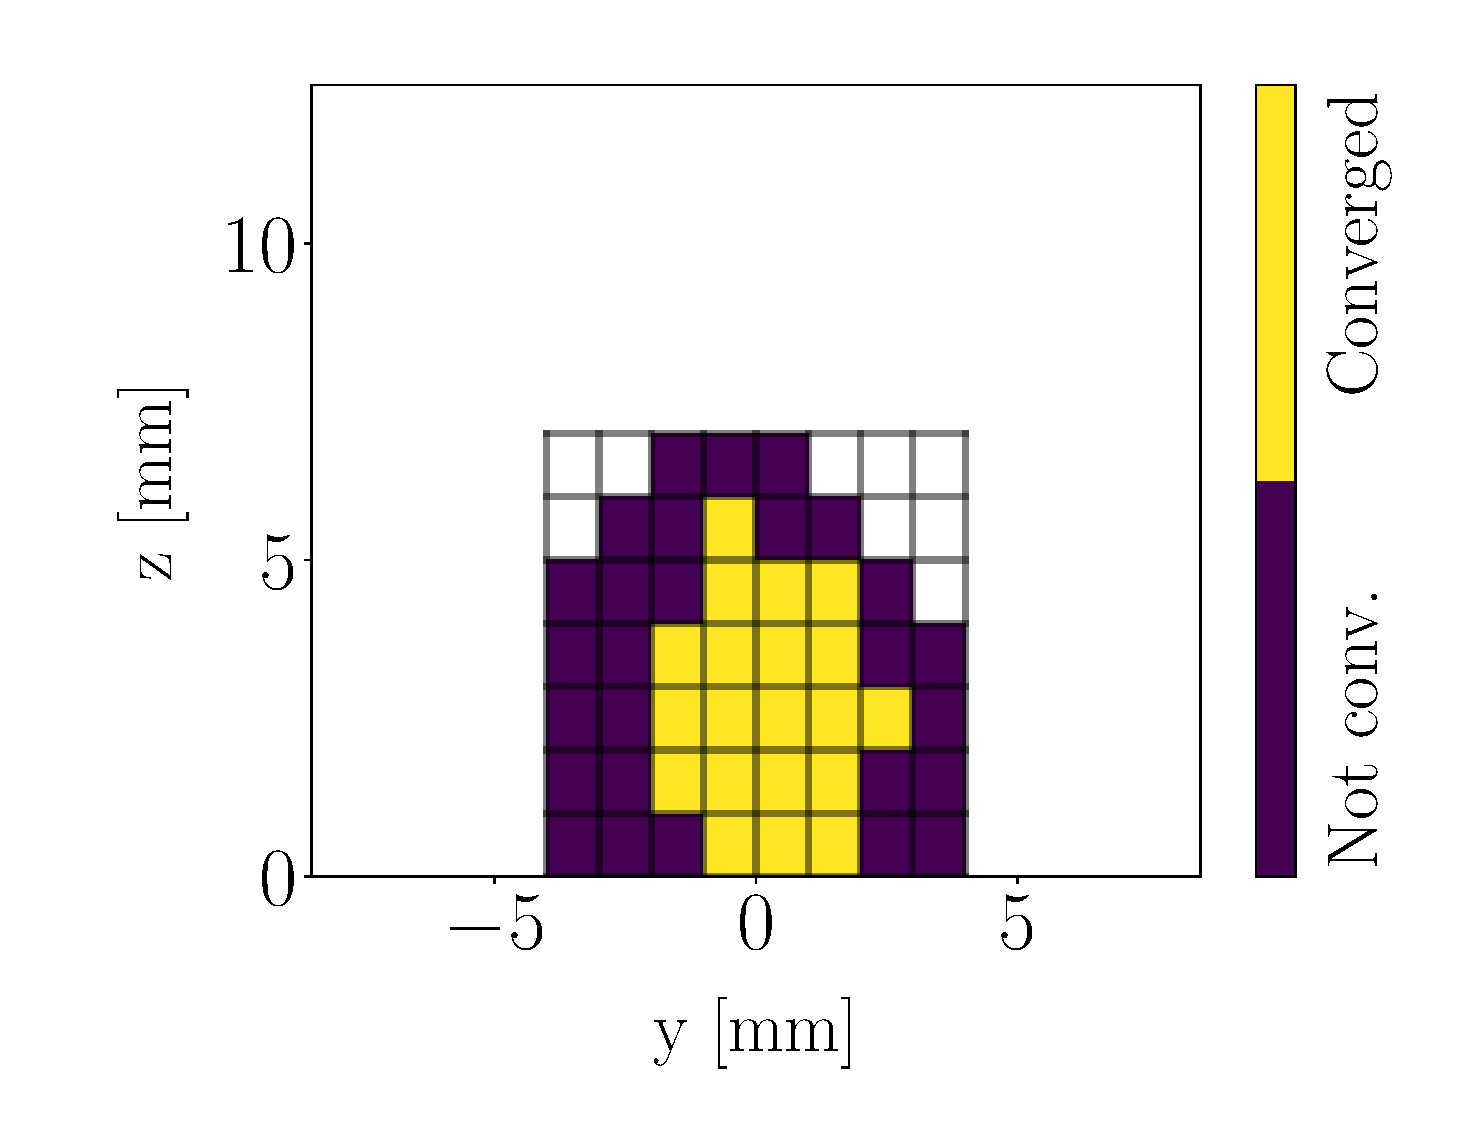
\includegraphics[scale=\scaleSLIJICF]{./part2_developments/figures_ch5_resolved_JICF/injectors_SLI/uG100_dx10_x05_convergence_map}
   %\caption{Case UG100\_DX10: crossflow planes}
   %\label{} 
\end{subfigure}

\vskip\baselineskip

\begin{subfigure}[b]{0.3\textwidth}
	\centering
   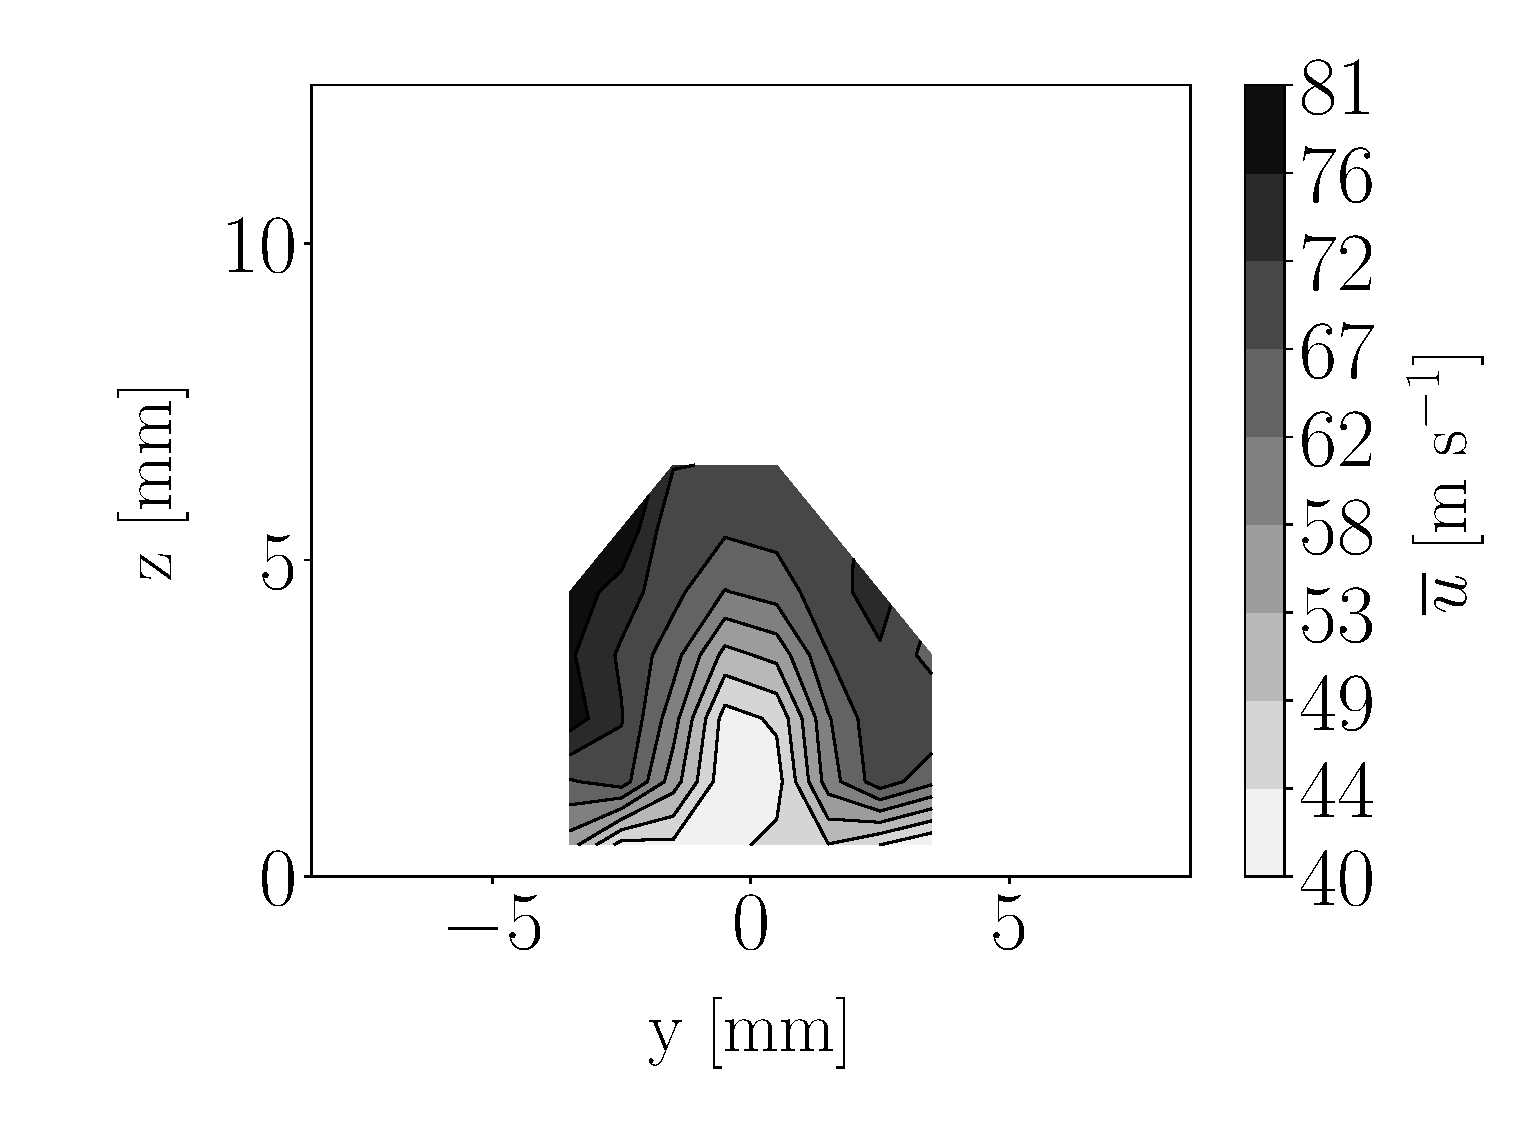
\includegraphics[scale=\scaleSLIJICF]{./part2_developments/figures_ch5_resolved_JICF/injectors_SLI/uG100_dx10_x05_ux_mean_map}
   %\caption{Case UG100\_DX20: crossflow planes}
   %\label{} 
\end{subfigure}
   \hspace{0.17in}
\begin{subfigure}[b]{0.3\textwidth}
	\centering
   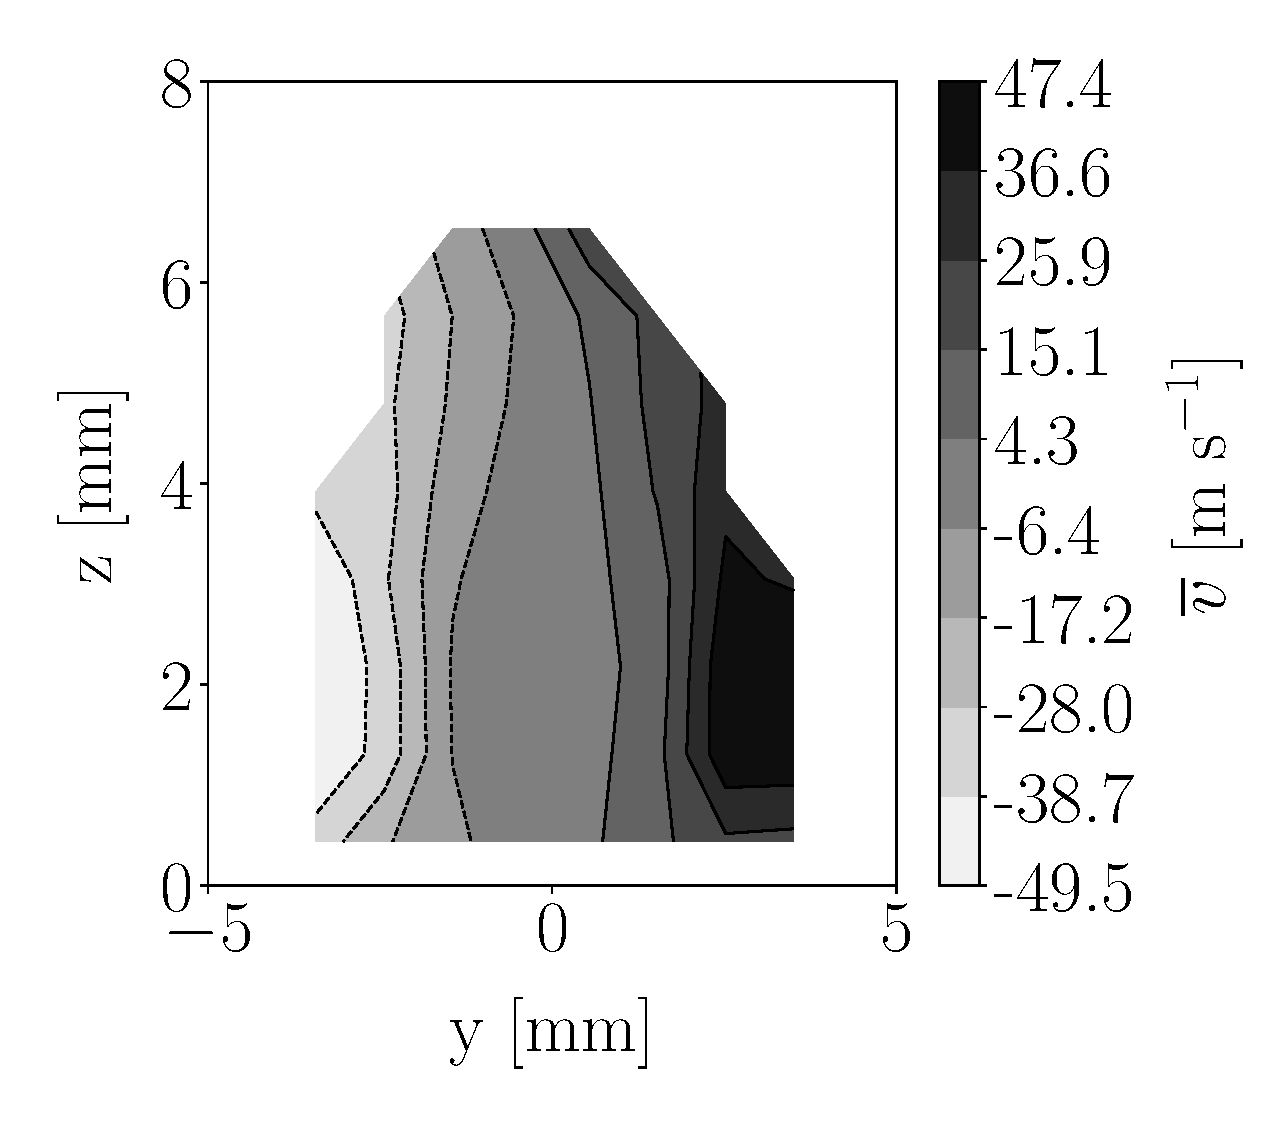
\includegraphics[scale=\scaleSLIJICF]{./part2_developments/figures_ch5_resolved_JICF/injectors_SLI/uG100_dx10_x05_uy_mean_map}
   %\caption{Case UG100\_DX20: filming planes}
   %\label{}
\end{subfigure}
   \hspace{0.17in}
\begin{subfigure}[b]{0.3\textwidth}
	\centering
   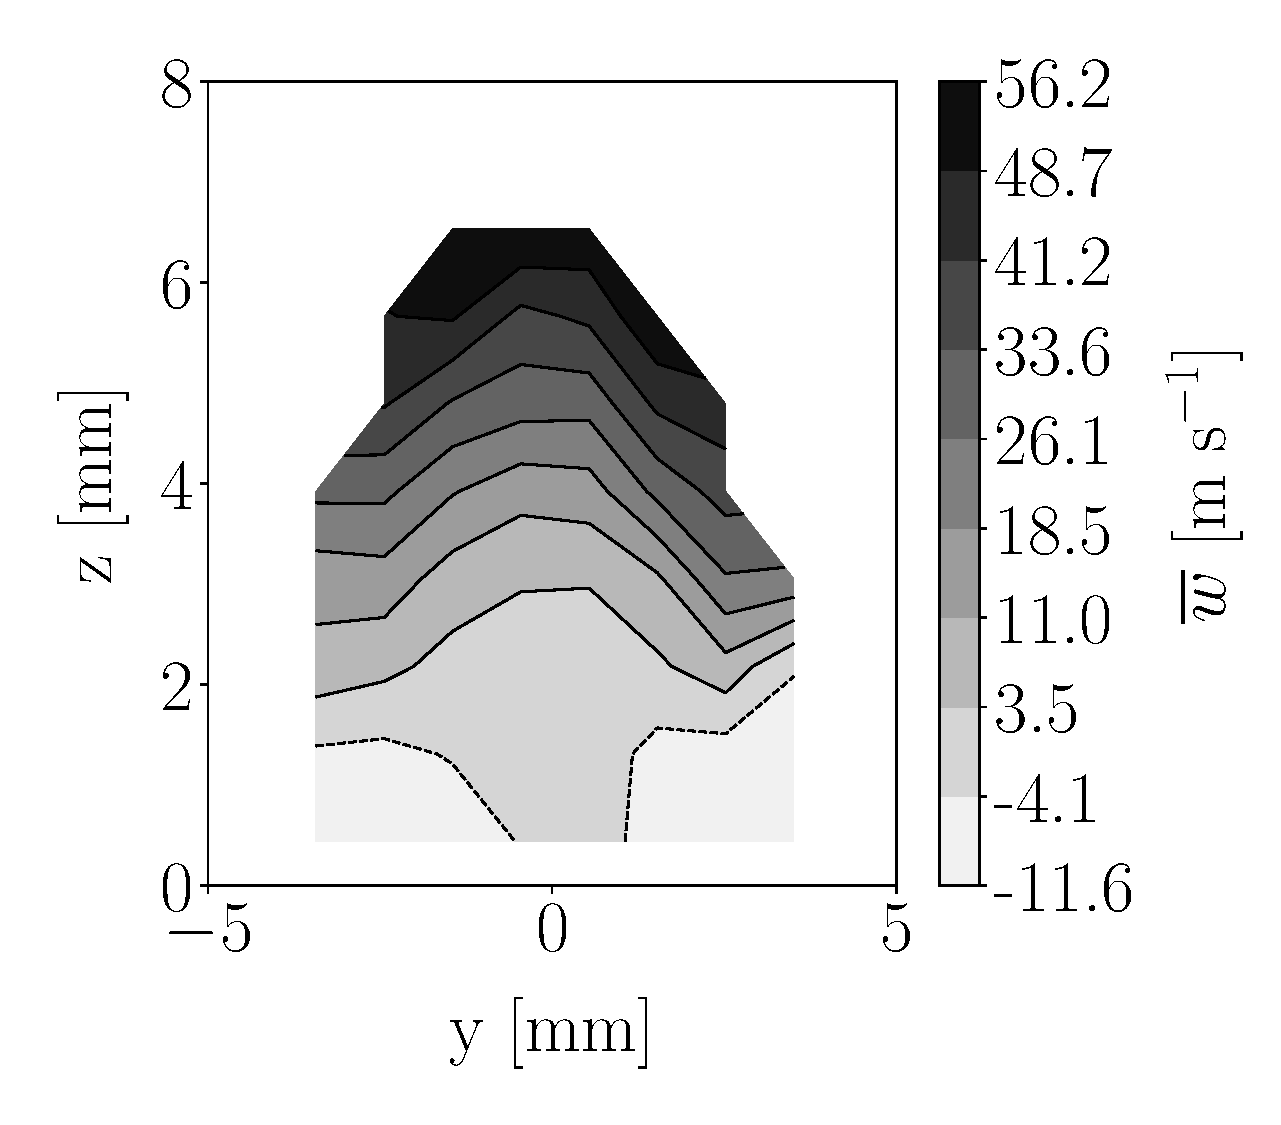
\includegraphics[scale=\scaleSLIJICF]{./part2_developments/figures_ch5_resolved_JICF/injectors_SLI/uG100_dx10_x05_uz_mean_map}
   %\caption{Case UG100\_DX10: crossflow planes}
   %\label{} 
\end{subfigure}
\caption{Spray states at x = 5 mm for case UG100\_DX10}
\label{fig:injectors_sli_uG100_dx10_x05}
\end{figure}


%%%%%%%%%%%%%%%% UG100_DX10, x = 10 mm


\begin{figure}[h!]
\centering\begin{subfigure}[b]{0.3\textwidth}
	\centering
   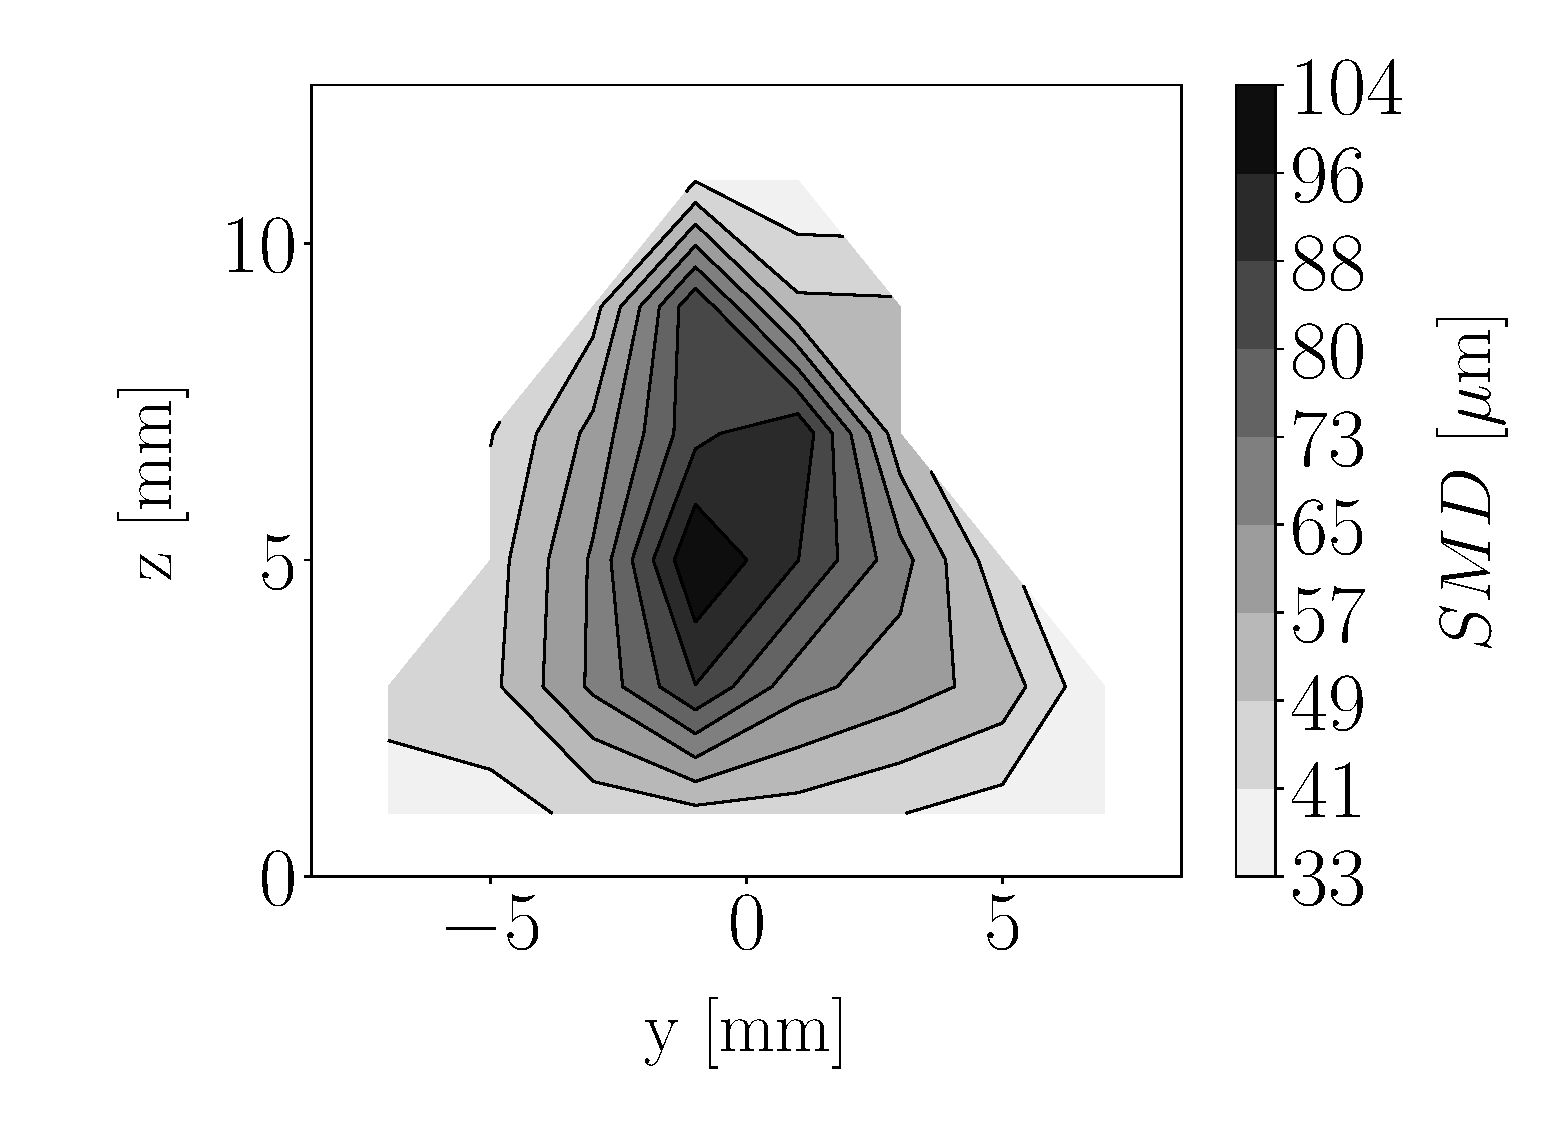
\includegraphics[scale=\scaleSLIJICF]{./part2_developments/figures_ch5_resolved_JICF/injectors_SLI/uG100_dx10_x10_SMD_map}
   %\caption{Case UG100\_DX20: crossflow planes}
   %\label{} 
\end{subfigure}
   \hspace{0.17in}
\begin{subfigure}[b]{0.3\textwidth}
	\centering
   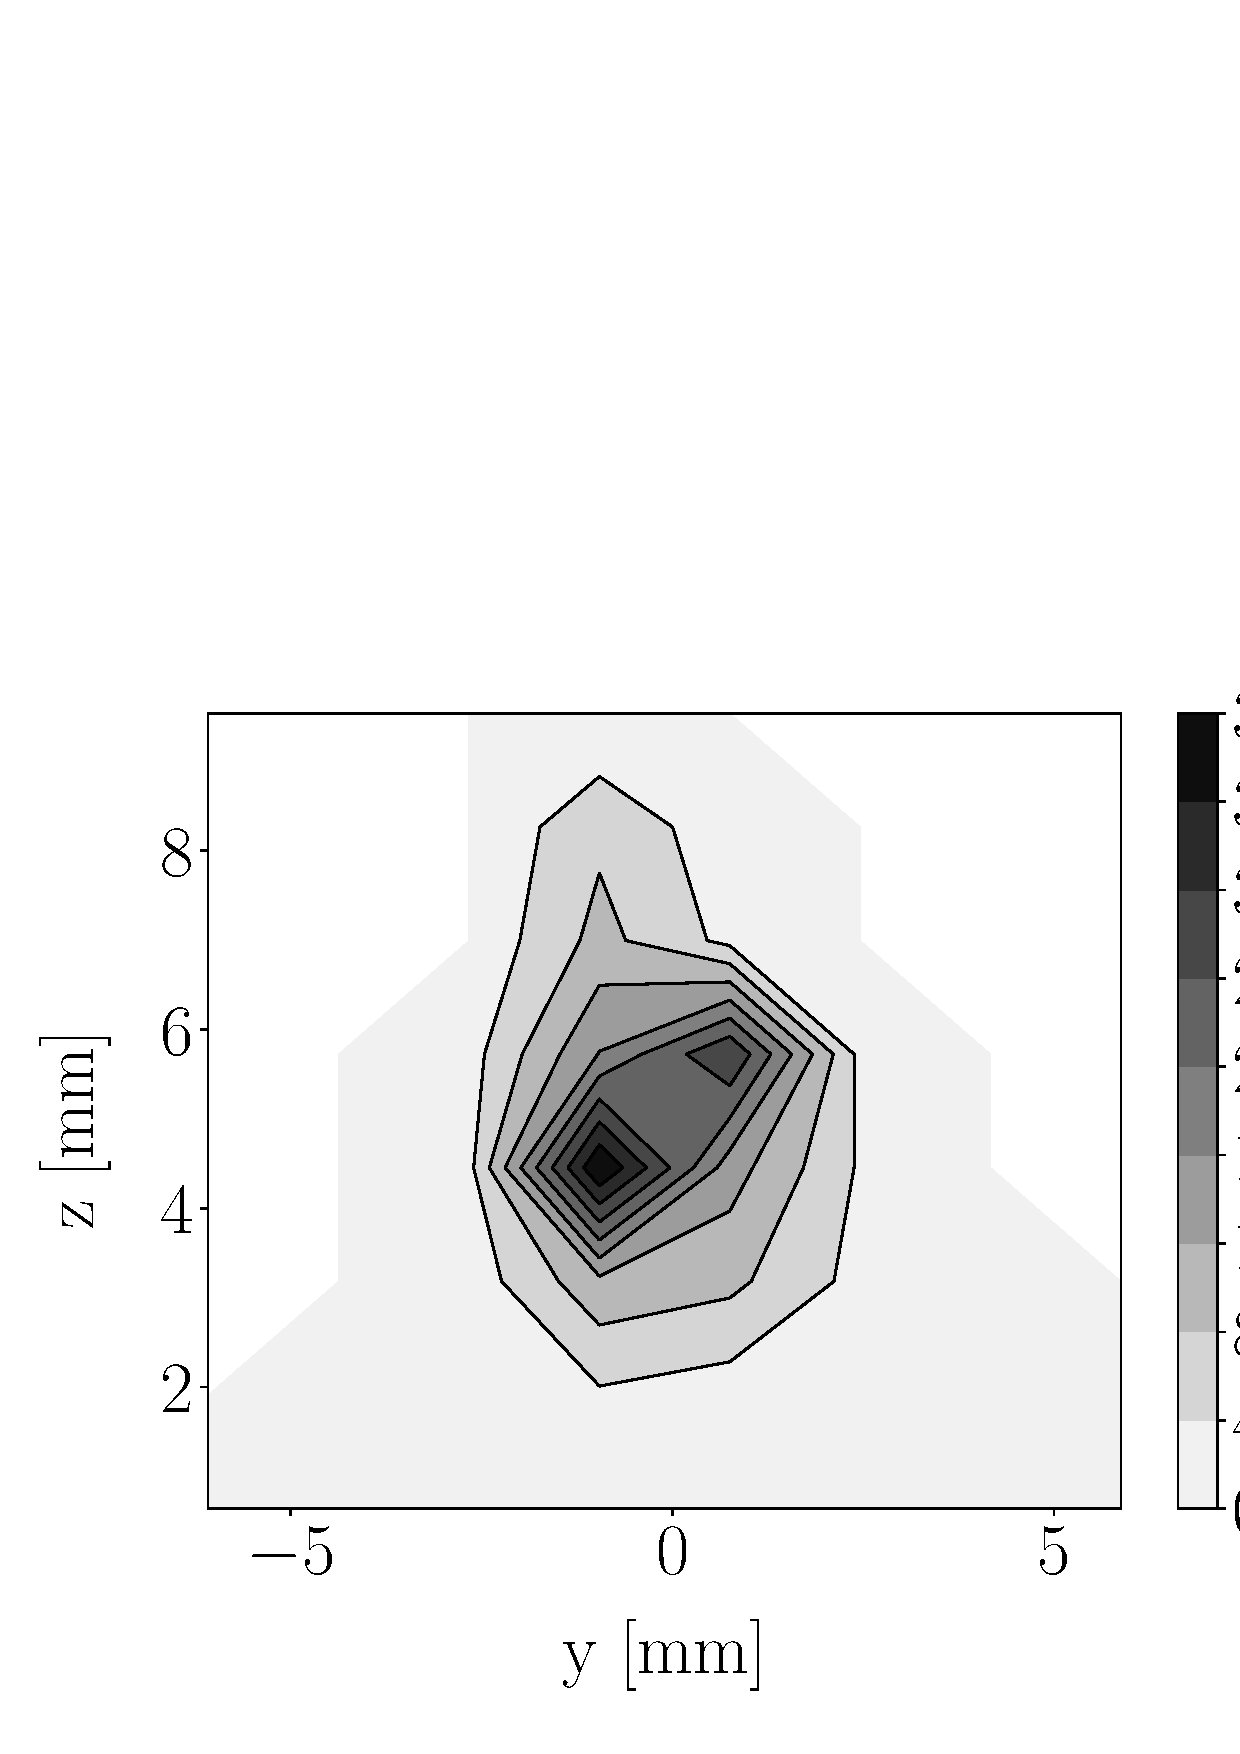
\includegraphics[scale=\scaleSLIJICF]{./part2_developments/figures_ch5_resolved_JICF/injectors_SLI/uG100_dx10_x10_volume_flux_map}
   %\caption{Case UG100\_DX20: filming planes}
   %\label{}
\end{subfigure}
   \hspace{0.17in}
\begin{subfigure}[b]{0.3\textwidth}
	\centering
   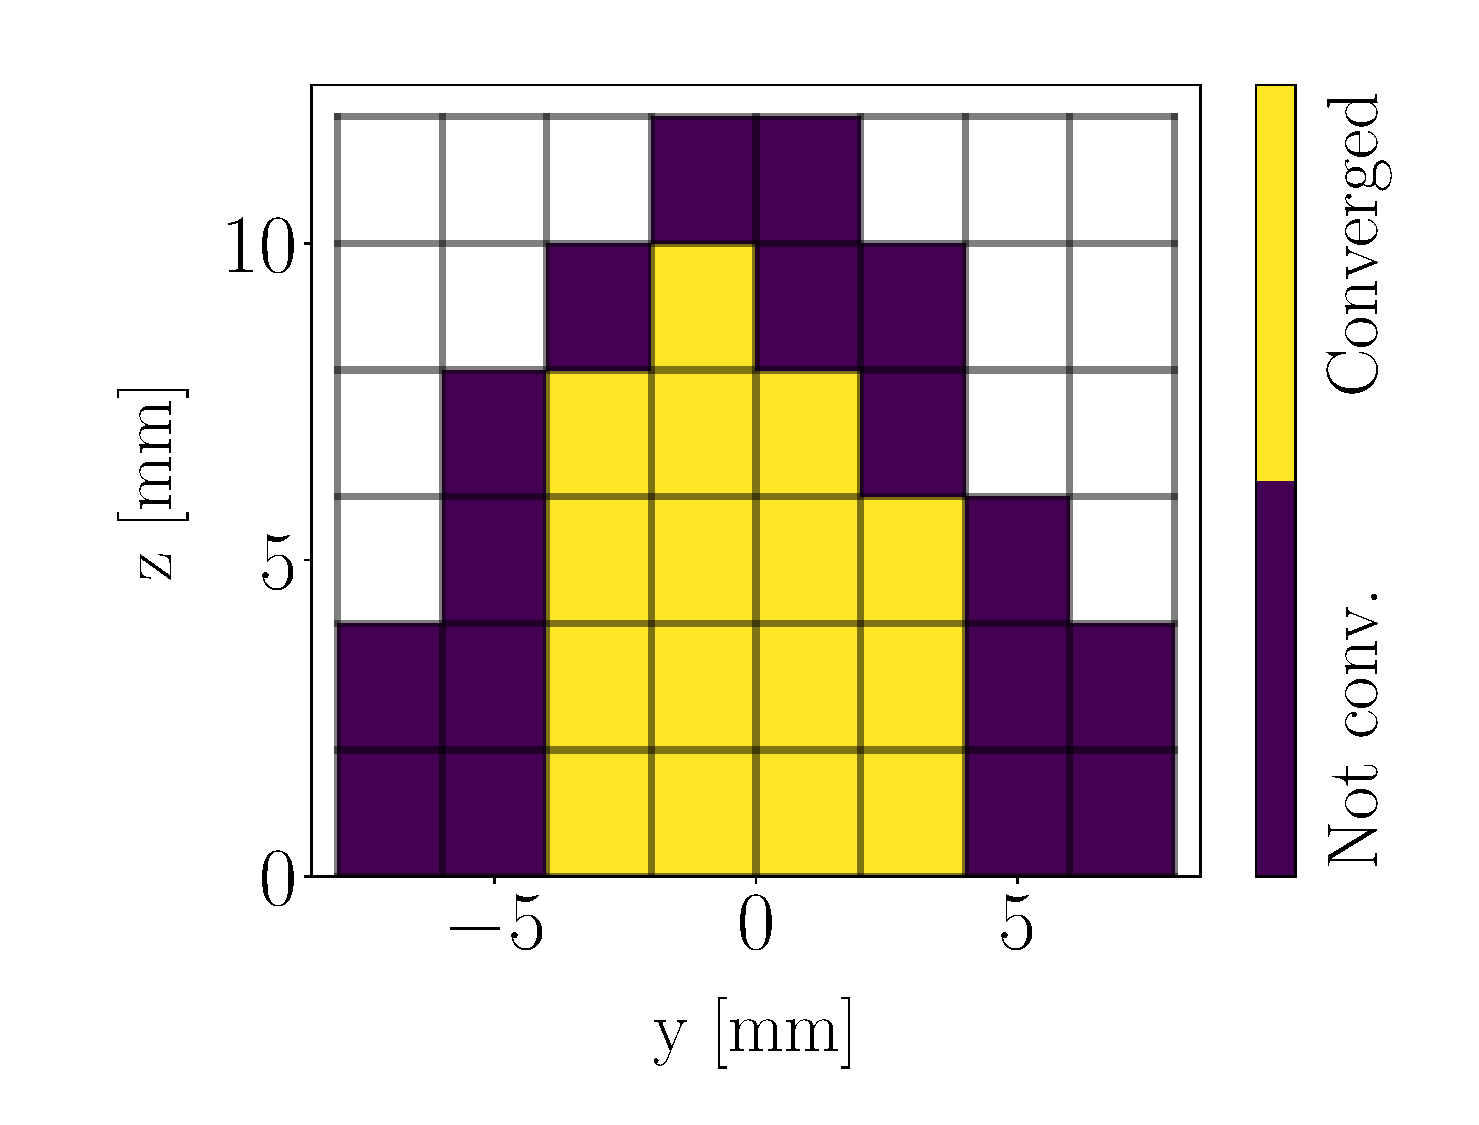
\includegraphics[scale=\scaleSLIJICF]{./part2_developments/figures_ch5_resolved_JICF/injectors_SLI/uG100_dx10_x10_convergence_map}
   %\caption{Case UG100\_DX10: crossflow planes}
   %\label{} 
\end{subfigure}

\vskip\baselineskip

\begin{subfigure}[b]{0.3\textwidth}
	\centering
   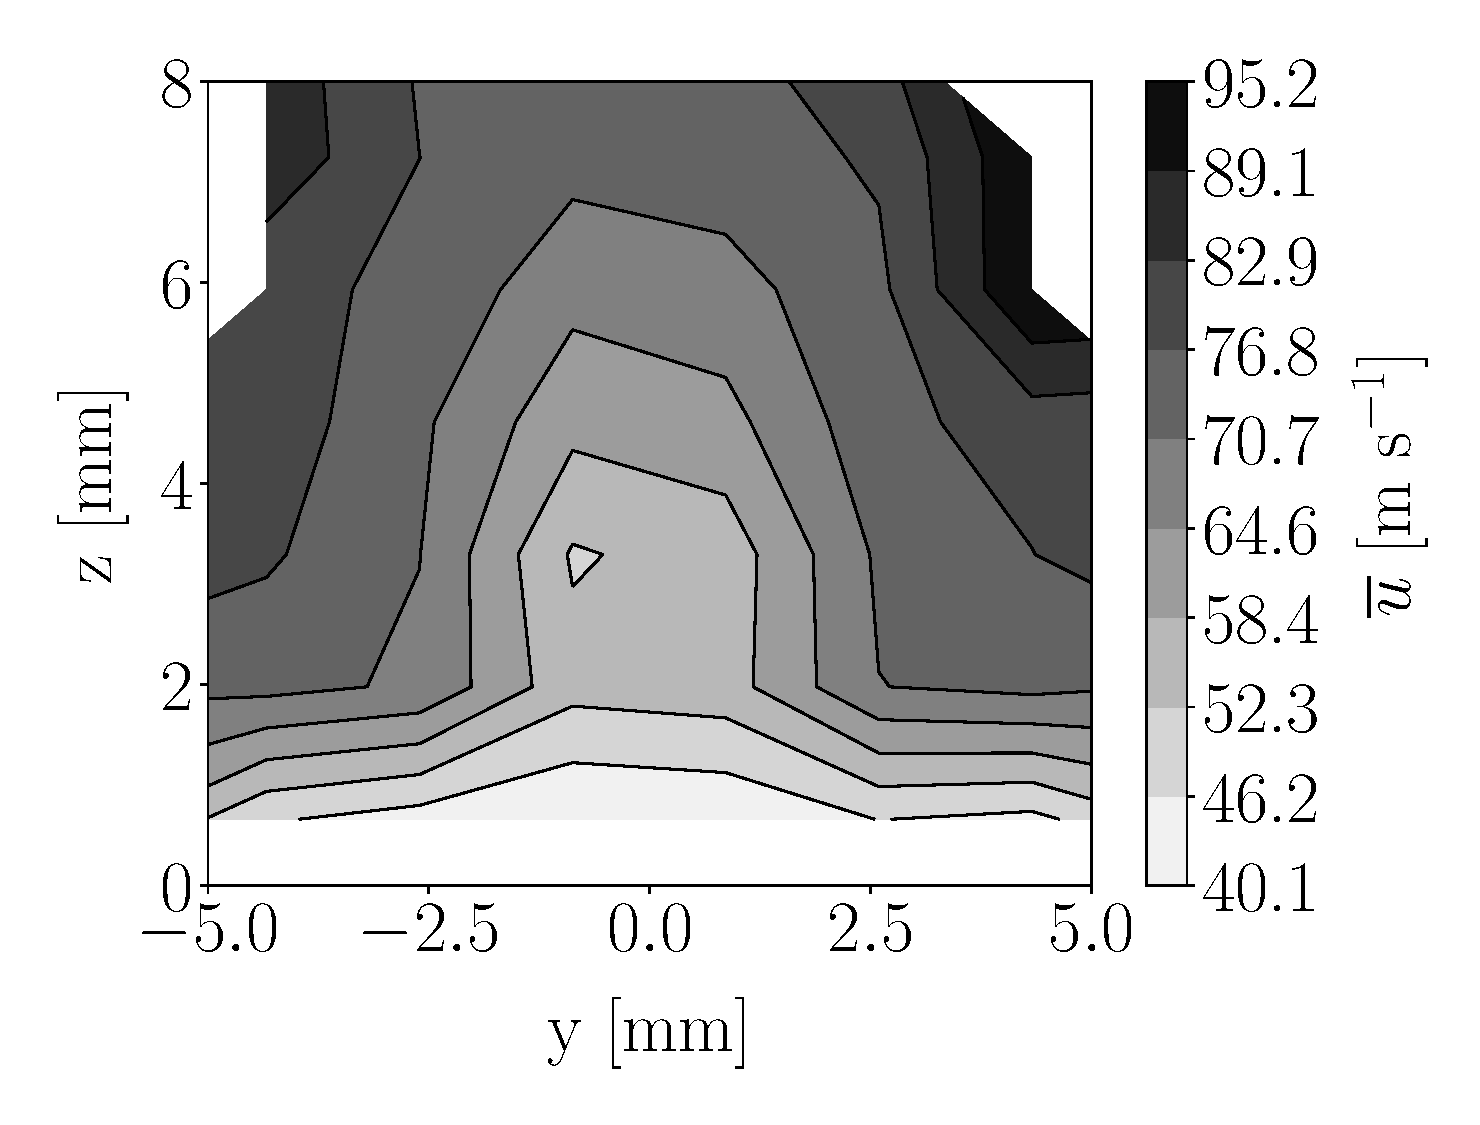
\includegraphics[scale=\scaleSLIJICF]{./part2_developments/figures_ch5_resolved_JICF/injectors_SLI/uG100_dx10_x10_ux_mean_map}
   %\caption{Case UG100\_DX20: crossflow planes}
   %\label{} 
\end{subfigure}
   \hspace{0.17in}
\begin{subfigure}[b]{0.3\textwidth}
	\centering
   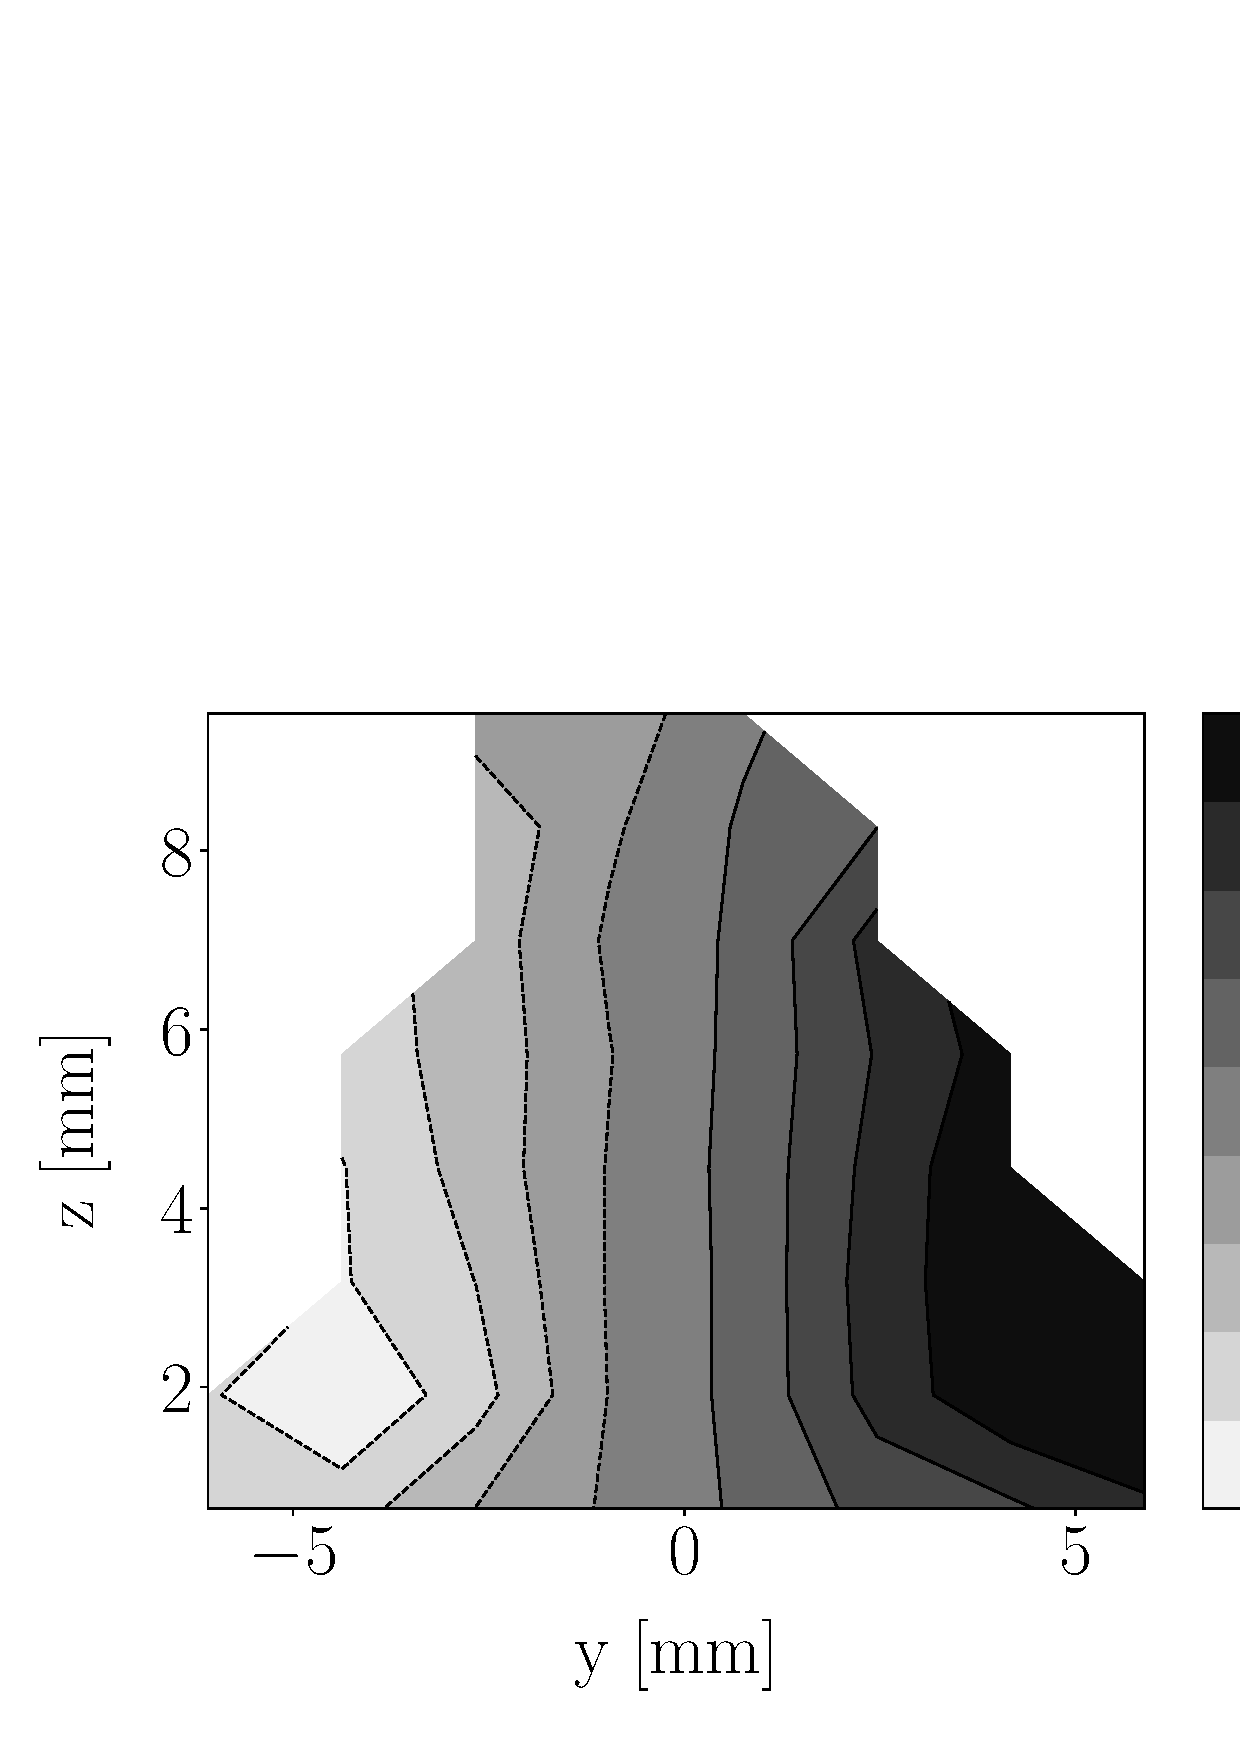
\includegraphics[scale=\scaleSLIJICF]{./part2_developments/figures_ch5_resolved_JICF/injectors_SLI/uG100_dx10_x10_uy_mean_map}
   %\caption{Case UG100\_DX20: filming planes}
   %\label{}
\end{subfigure}
   \hspace{0.17in}
\begin{subfigure}[b]{0.3\textwidth}
	\centering
   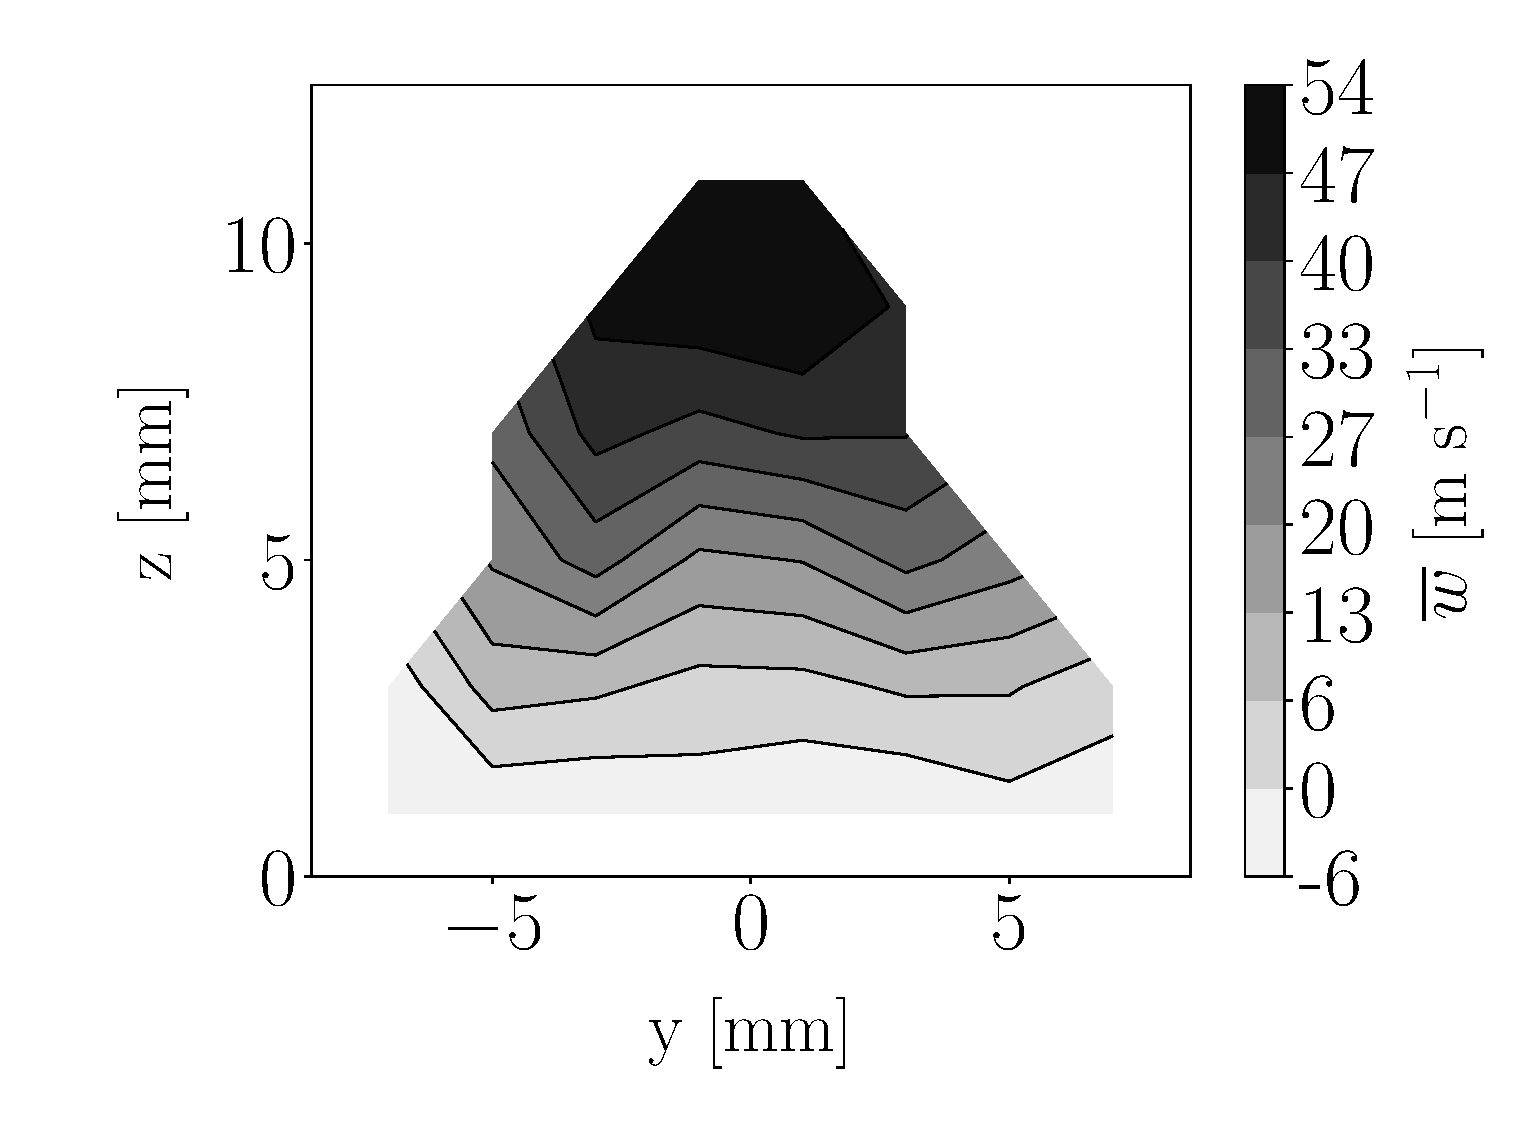
\includegraphics[scale=\scaleSLIJICF]{./part2_developments/figures_ch5_resolved_JICF/injectors_SLI/uG100_dx10_x10_uz_mean_map}
   %\caption{Case UG100\_DX10: crossflow planes}
   %\label{} 
\end{subfigure}
\caption{Spray states at x = 10 mm for case UG100\_DX10}
\label{fig:injectors_sli_uG100_dx10_x10}
\end{figure}


\clearpage

\subsubsection*{Case UG100\_DX20}



%%%%%%%%%%%%%%%% UG100_DX20, x = 5 mm


\begin{figure}[h!]
\centering
\begin{subfigure}[b]{0.3\textwidth}
	\centering
   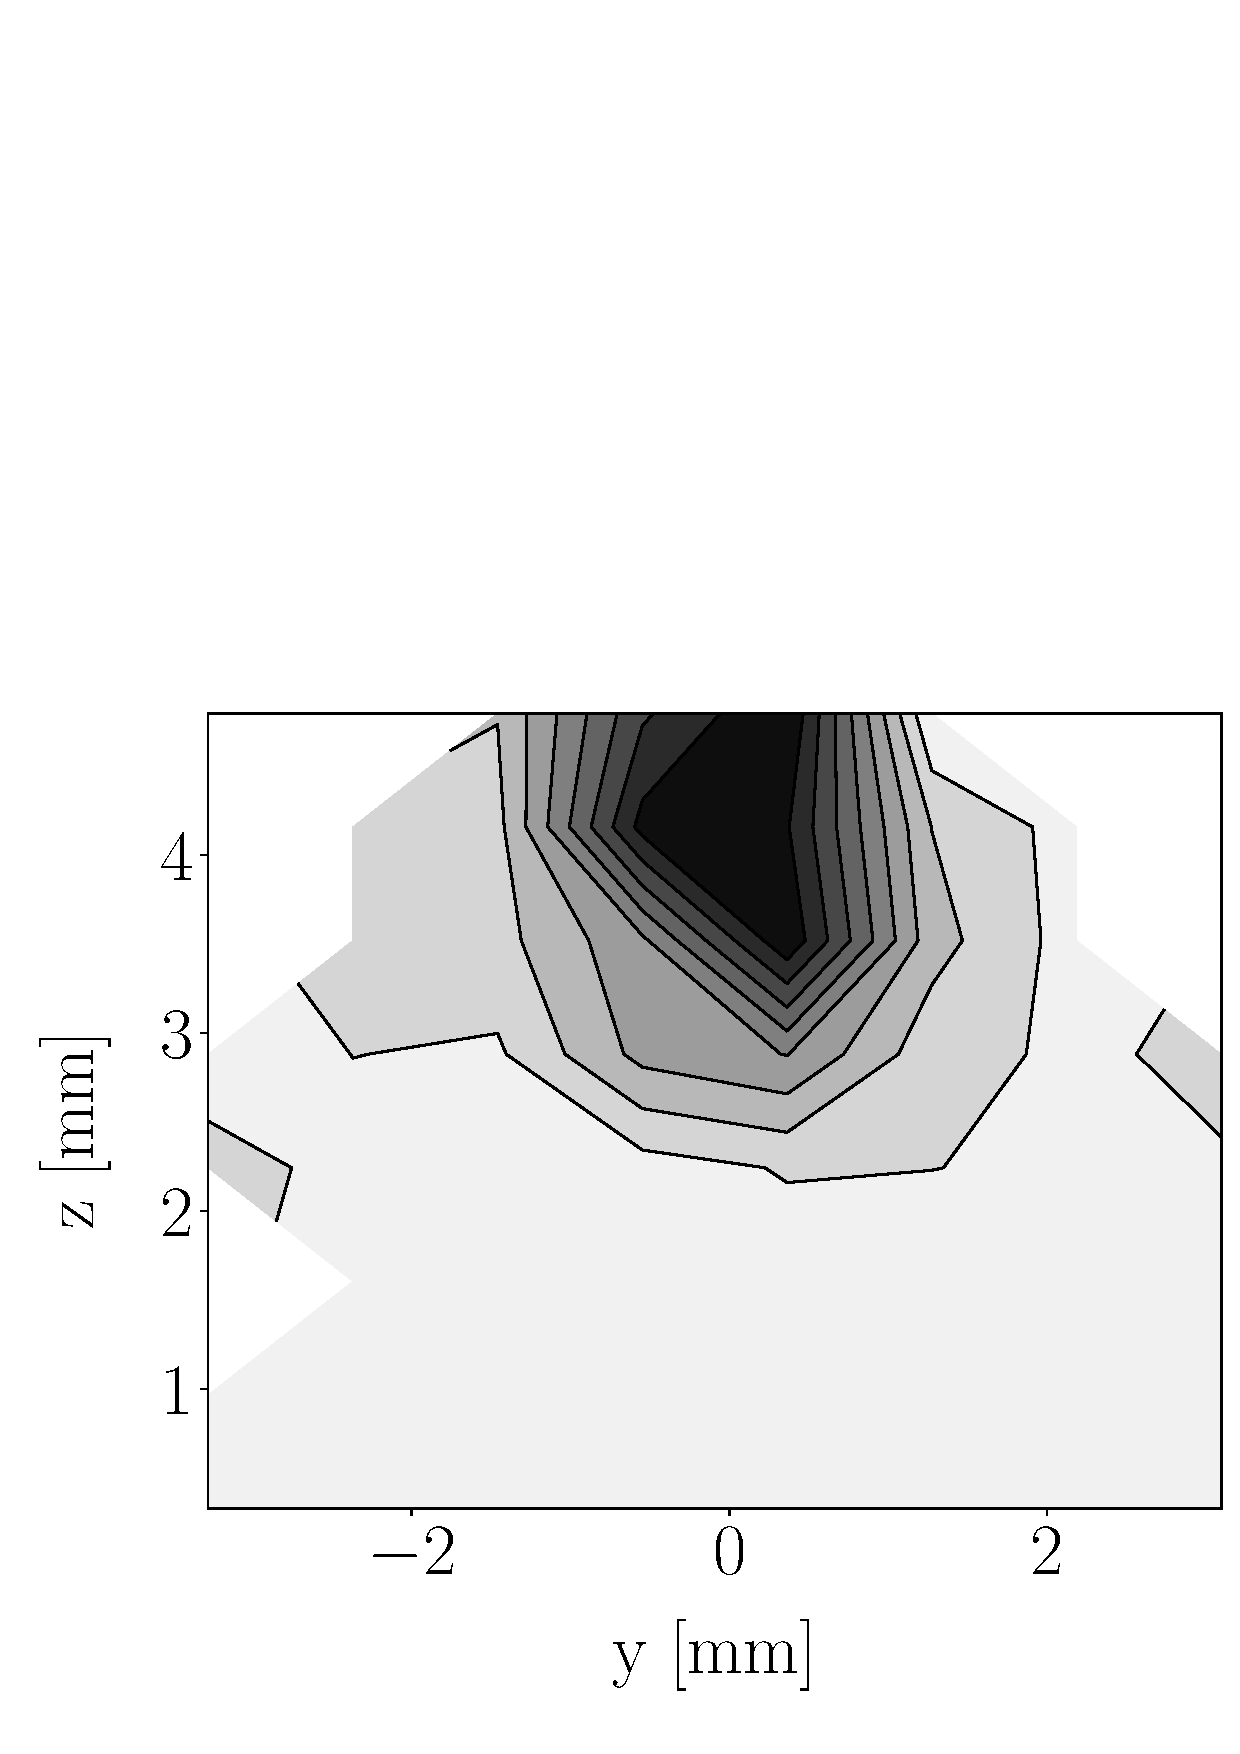
\includegraphics[scale=\scaleSLIJICF]{./part2_developments/figures_ch5_resolved_JICF/injectors_SLI/uG100_dx20_x05_SMD_map}
   %\caption{Case UG100\_DX20: crossflow planes}
   %\label{} 
\end{subfigure}
   \hspace{0.17in}
\begin{subfigure}[b]{0.3\textwidth}
	\centering
   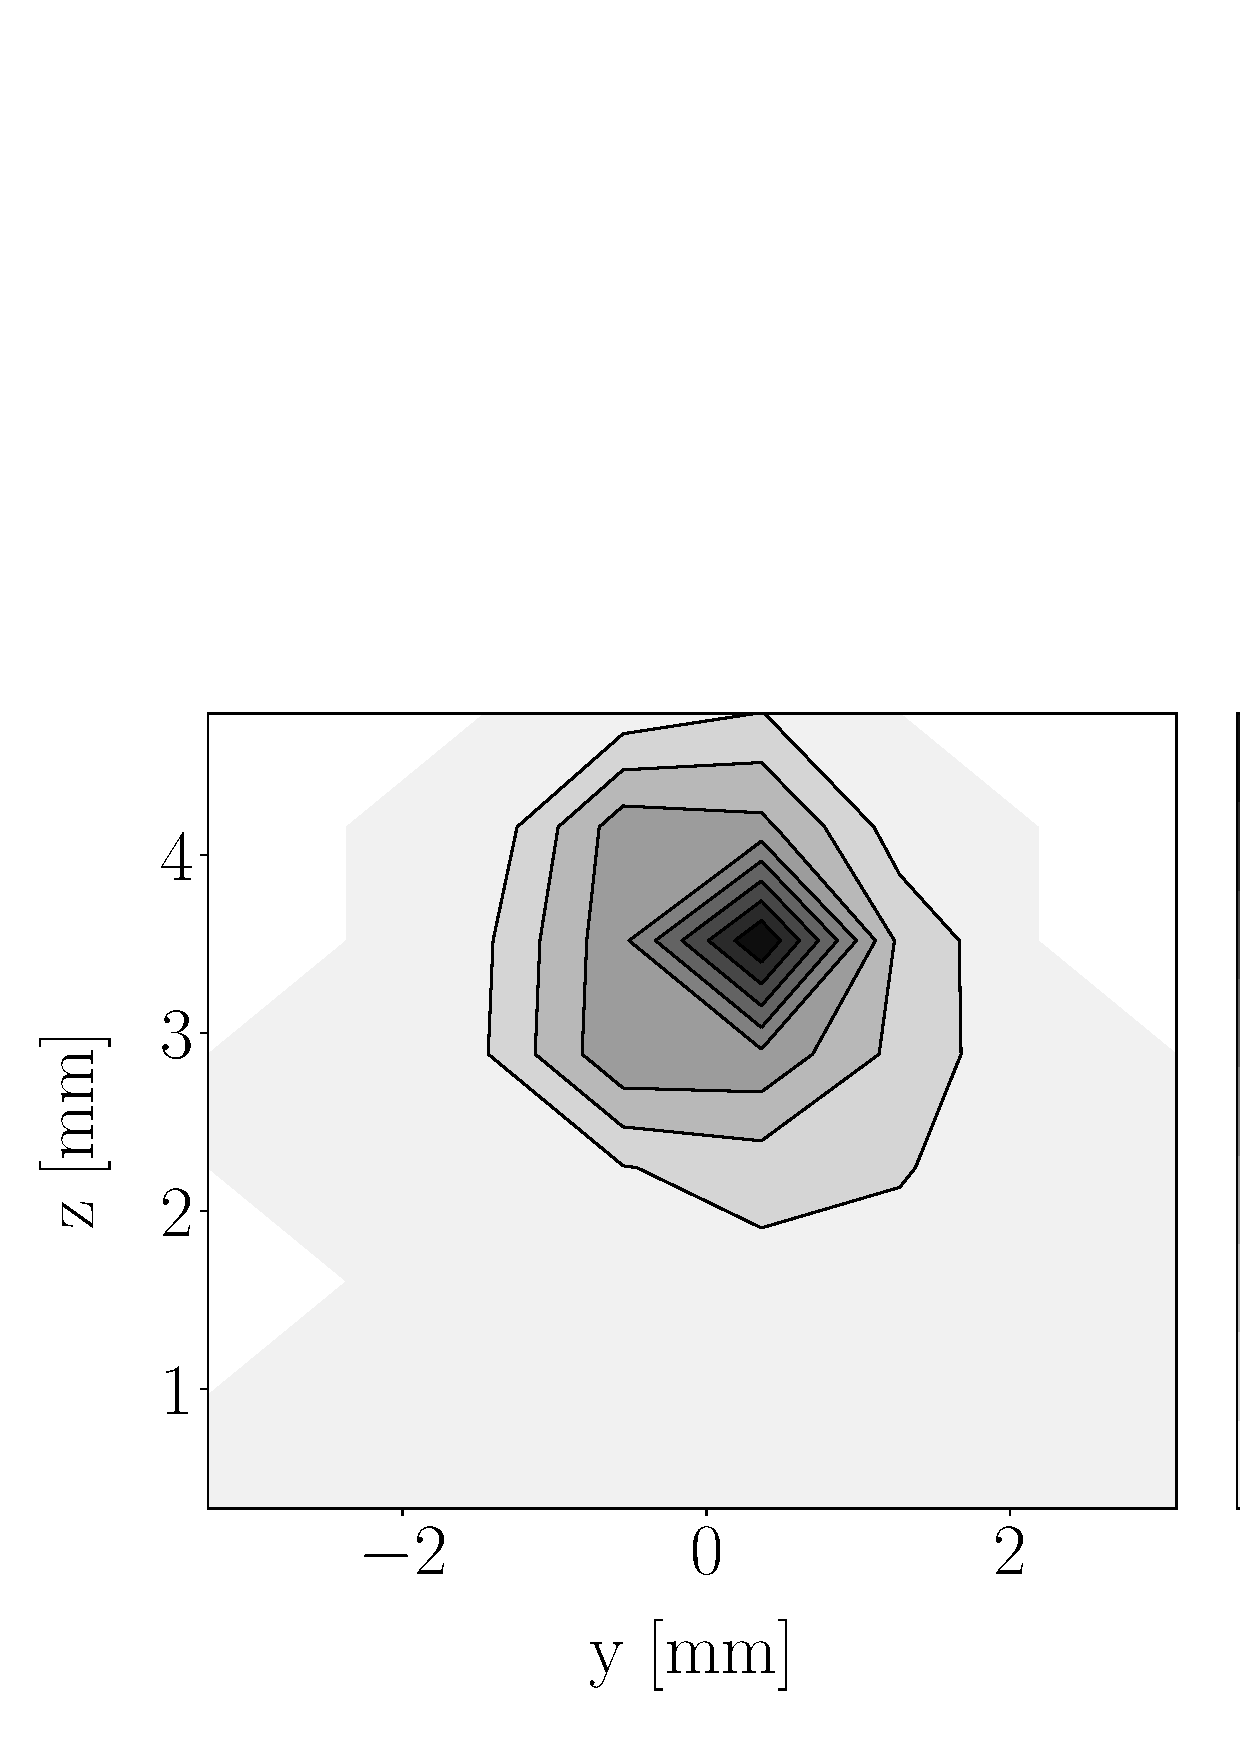
\includegraphics[scale=\scaleSLIJICF]{./part2_developments/figures_ch5_resolved_JICF/injectors_SLI/uG100_dx20_x05_volume_flux_map}
   %\caption{Case UG100\_DX20: filming planes}
   %\label{}
\end{subfigure}
   \hspace{0.17in}
\begin{subfigure}[b]{0.3\textwidth}
	\centering
   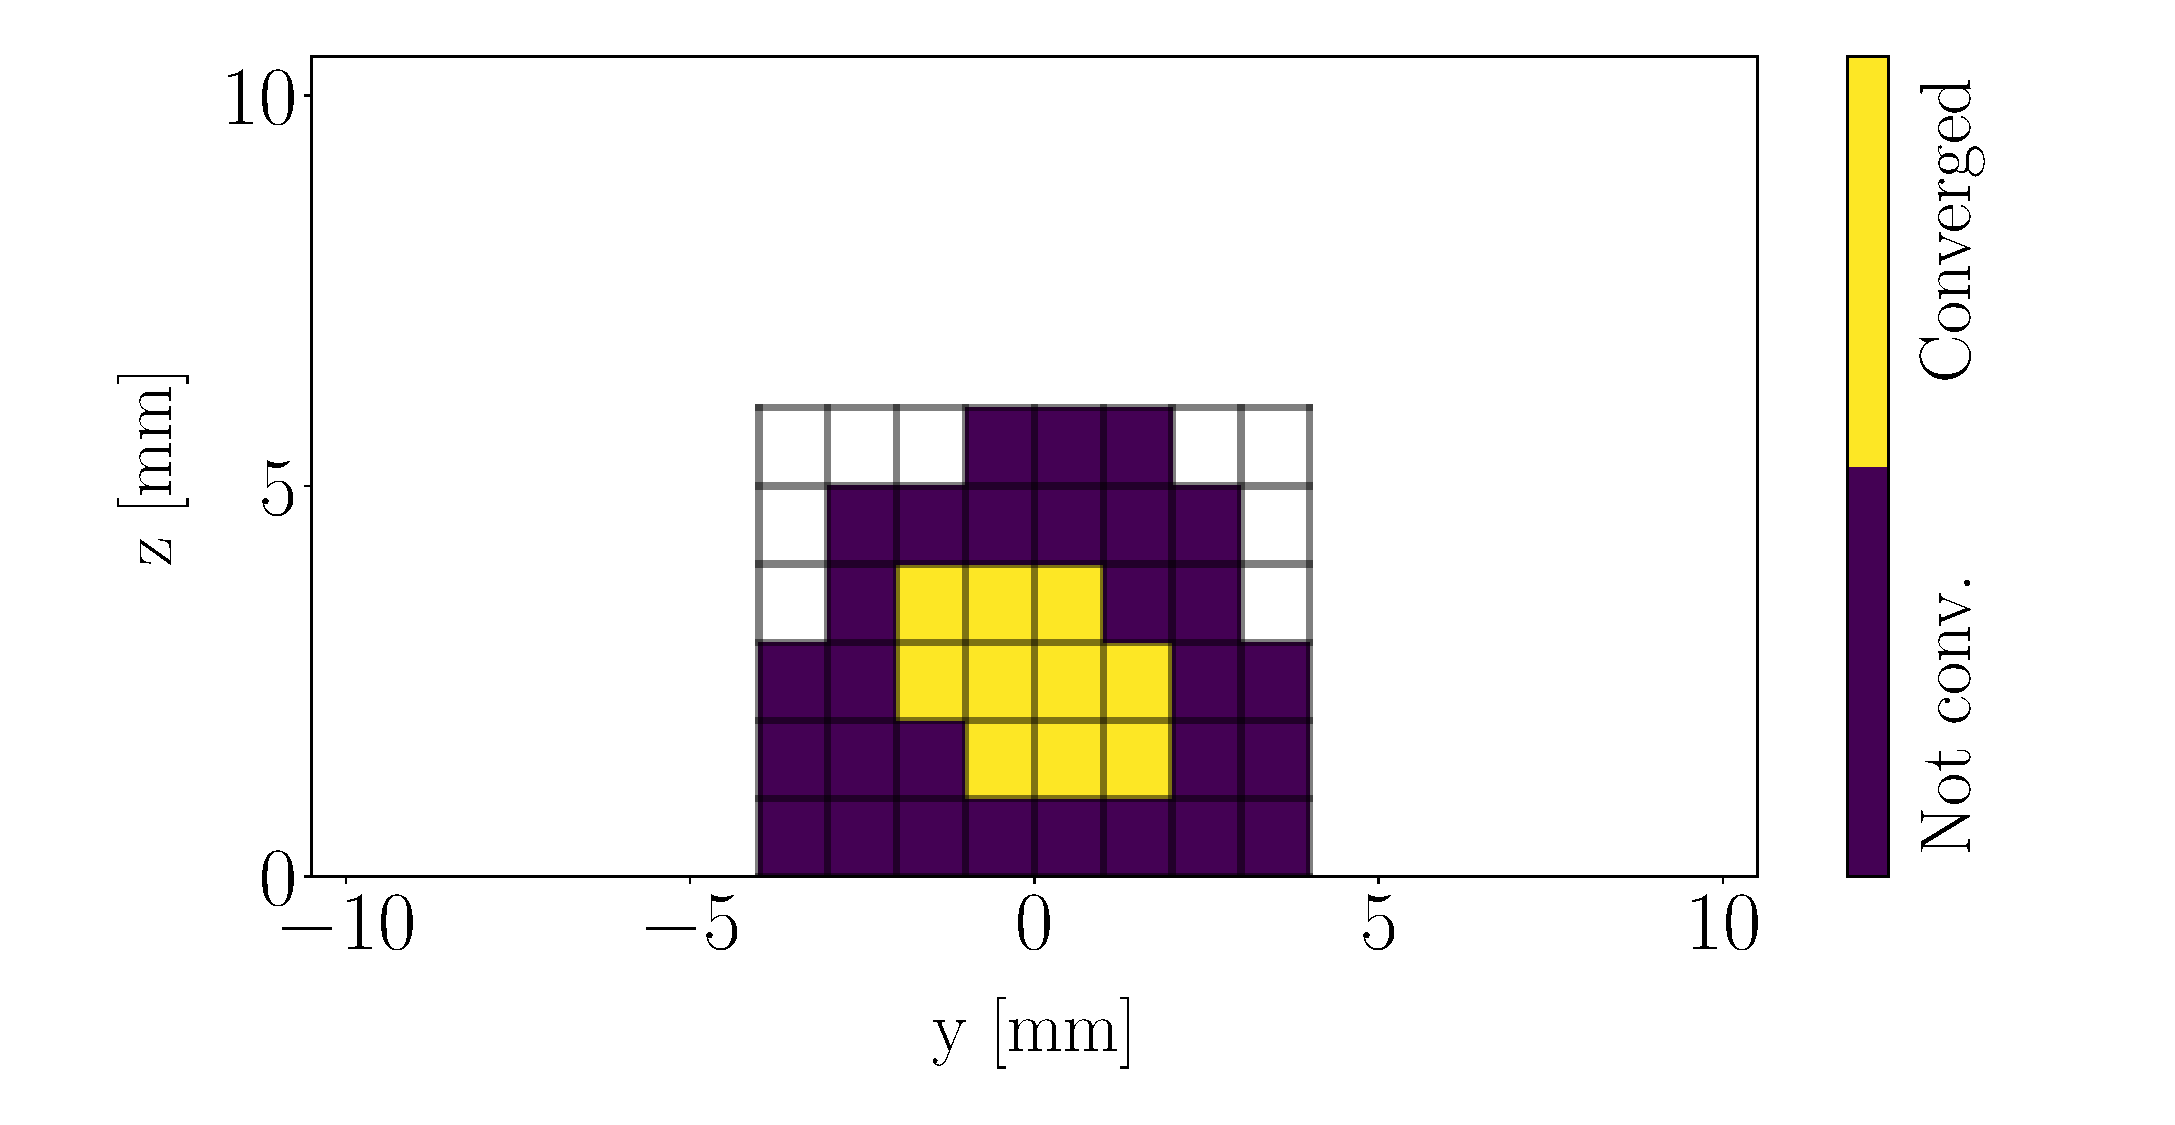
\includegraphics[scale=\scaleSLIJICF]{./part2_developments/figures_ch5_resolved_JICF/injectors_SLI/uG100_dx20_x05_convergence_map}
   %\caption{Case UG100\_DX10: crossflow planes}
   %\label{} 
\end{subfigure}

\vskip\baselineskip

\begin{subfigure}[b]{0.3\textwidth}
	\centering
   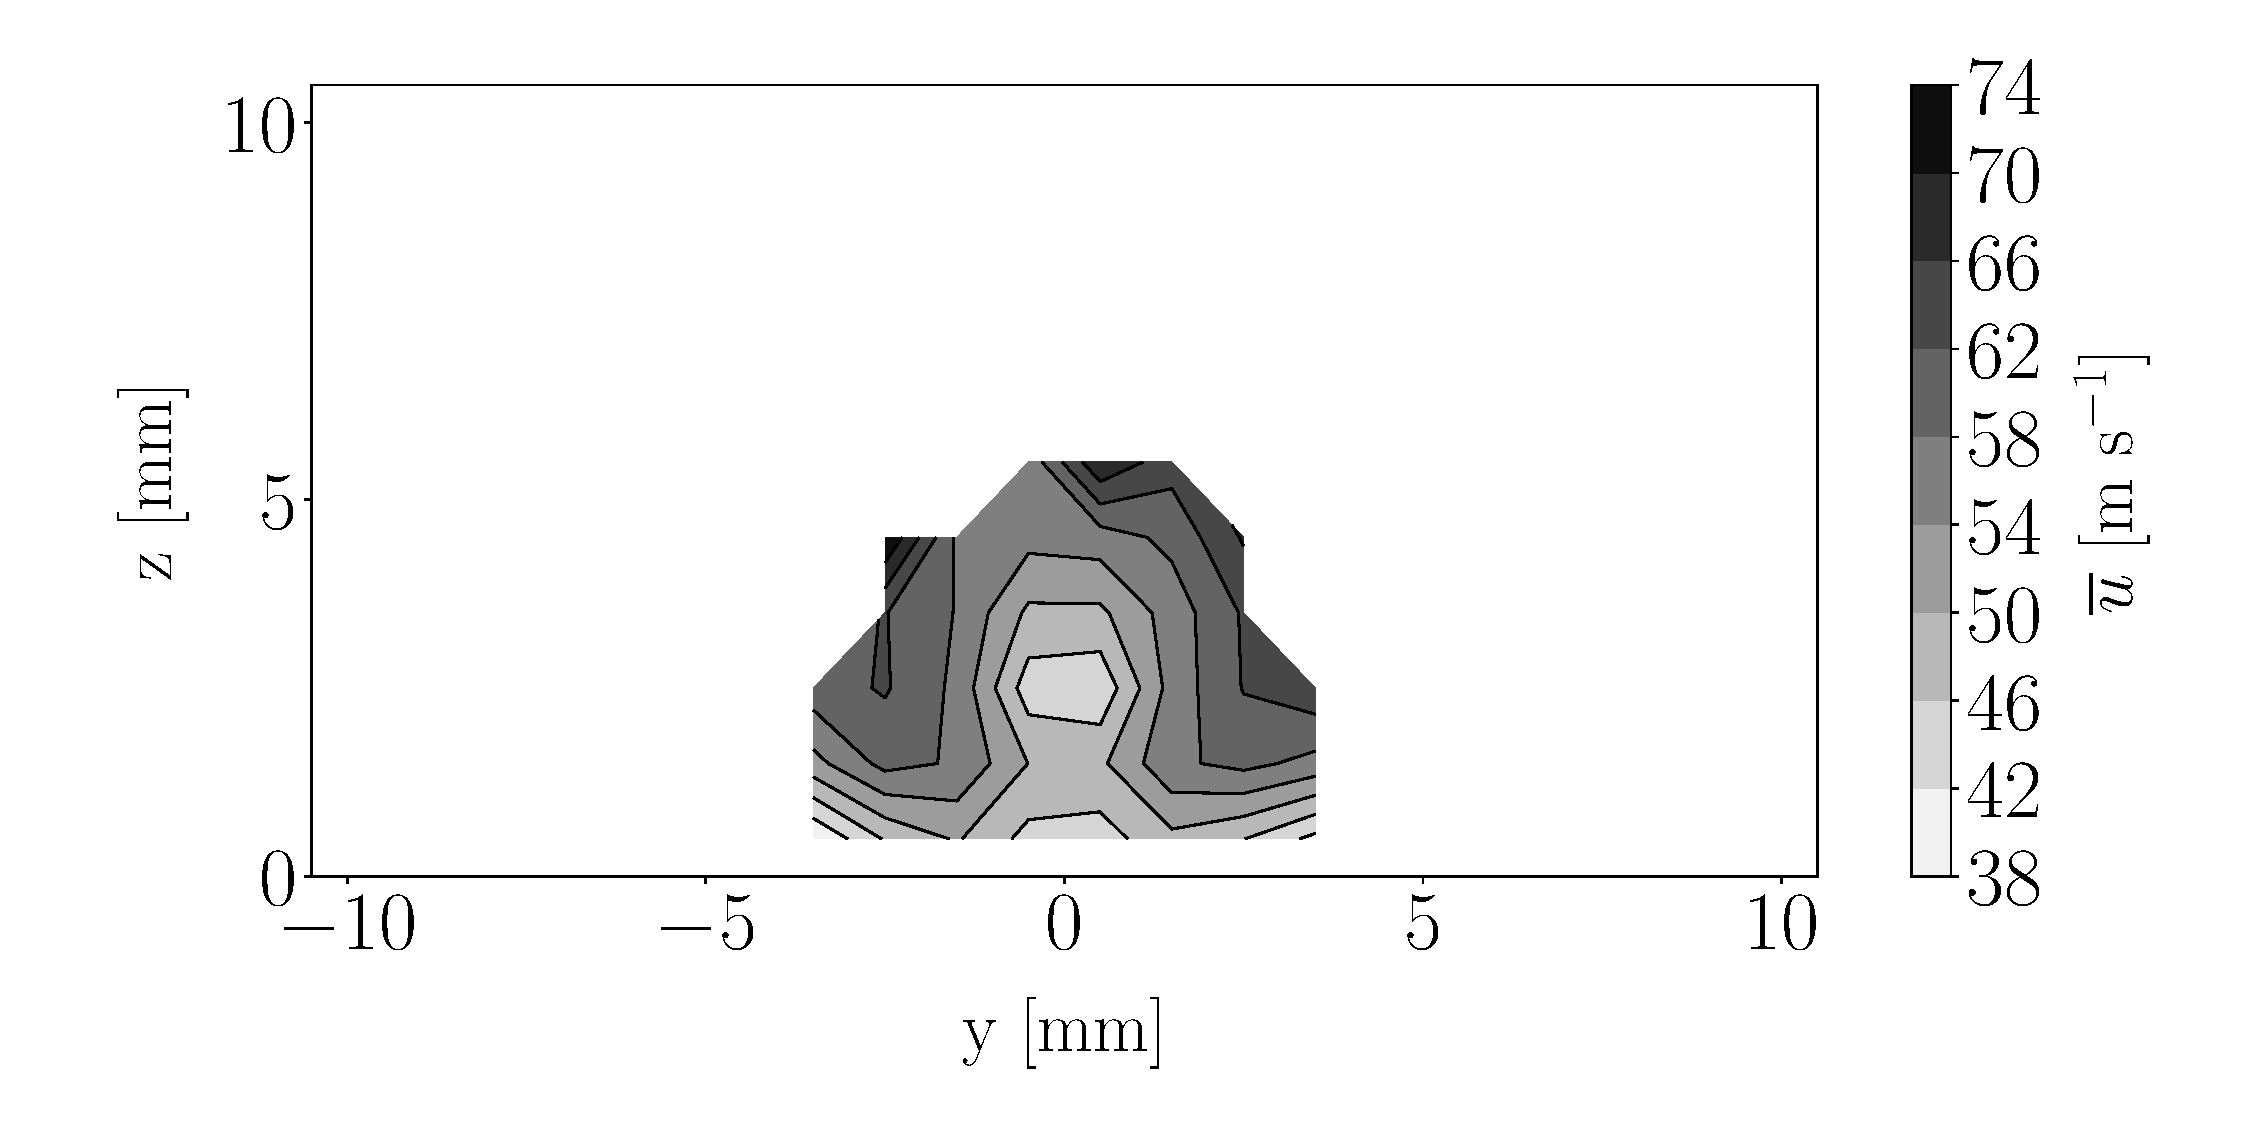
\includegraphics[scale=\scaleSLIJICF]{./part2_developments/figures_ch5_resolved_JICF/injectors_SLI/uG100_dx20_x05_ux_mean_map}
   %\caption{Case UG100\_DX20: crossflow planes}
   %\label{} 
\end{subfigure}
   \hspace{0.17in}
\begin{subfigure}[b]{0.3\textwidth}
	\centering
   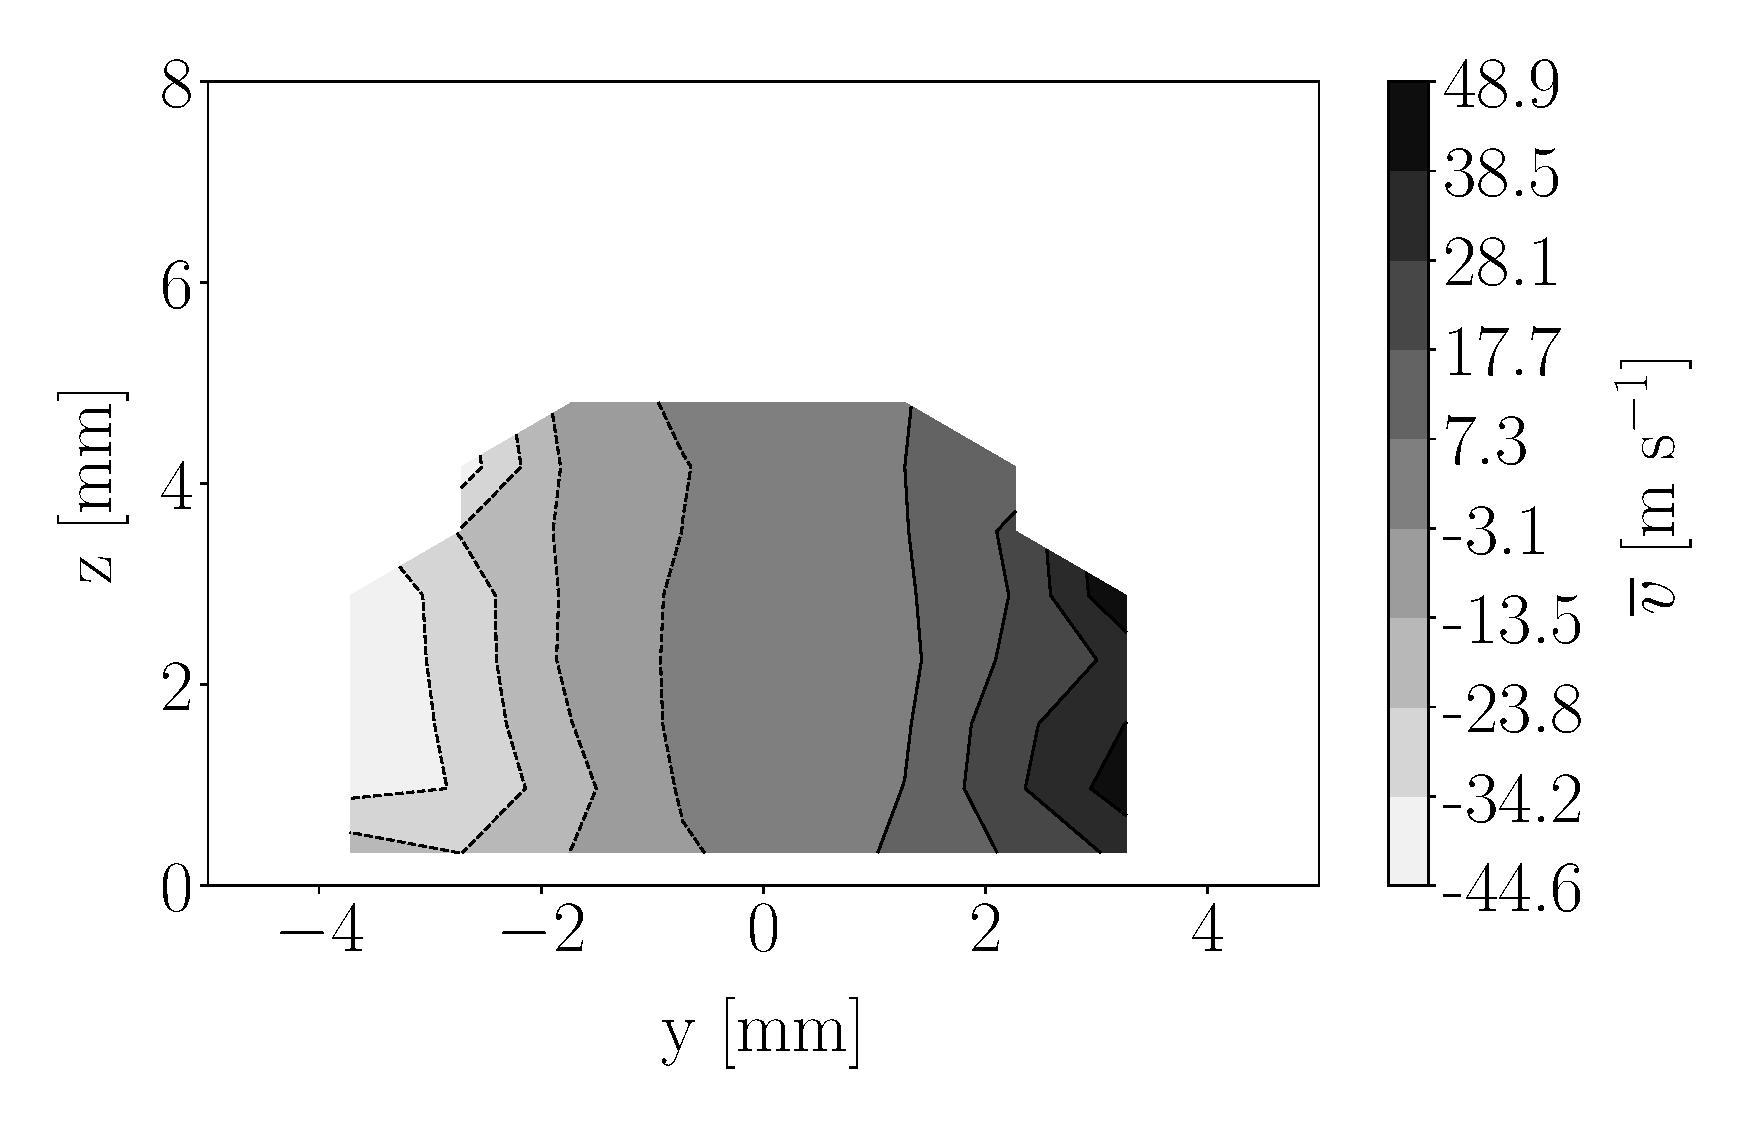
\includegraphics[scale=\scaleSLIJICF]{./part2_developments/figures_ch5_resolved_JICF/injectors_SLI/uG100_dx20_x05_uy_mean_map}
   %\caption{Case UG100\_DX20: filming planes}
   %\label{}
\end{subfigure}
   \hspace{0.17in}
\begin{subfigure}[b]{0.3\textwidth}
	\centering
   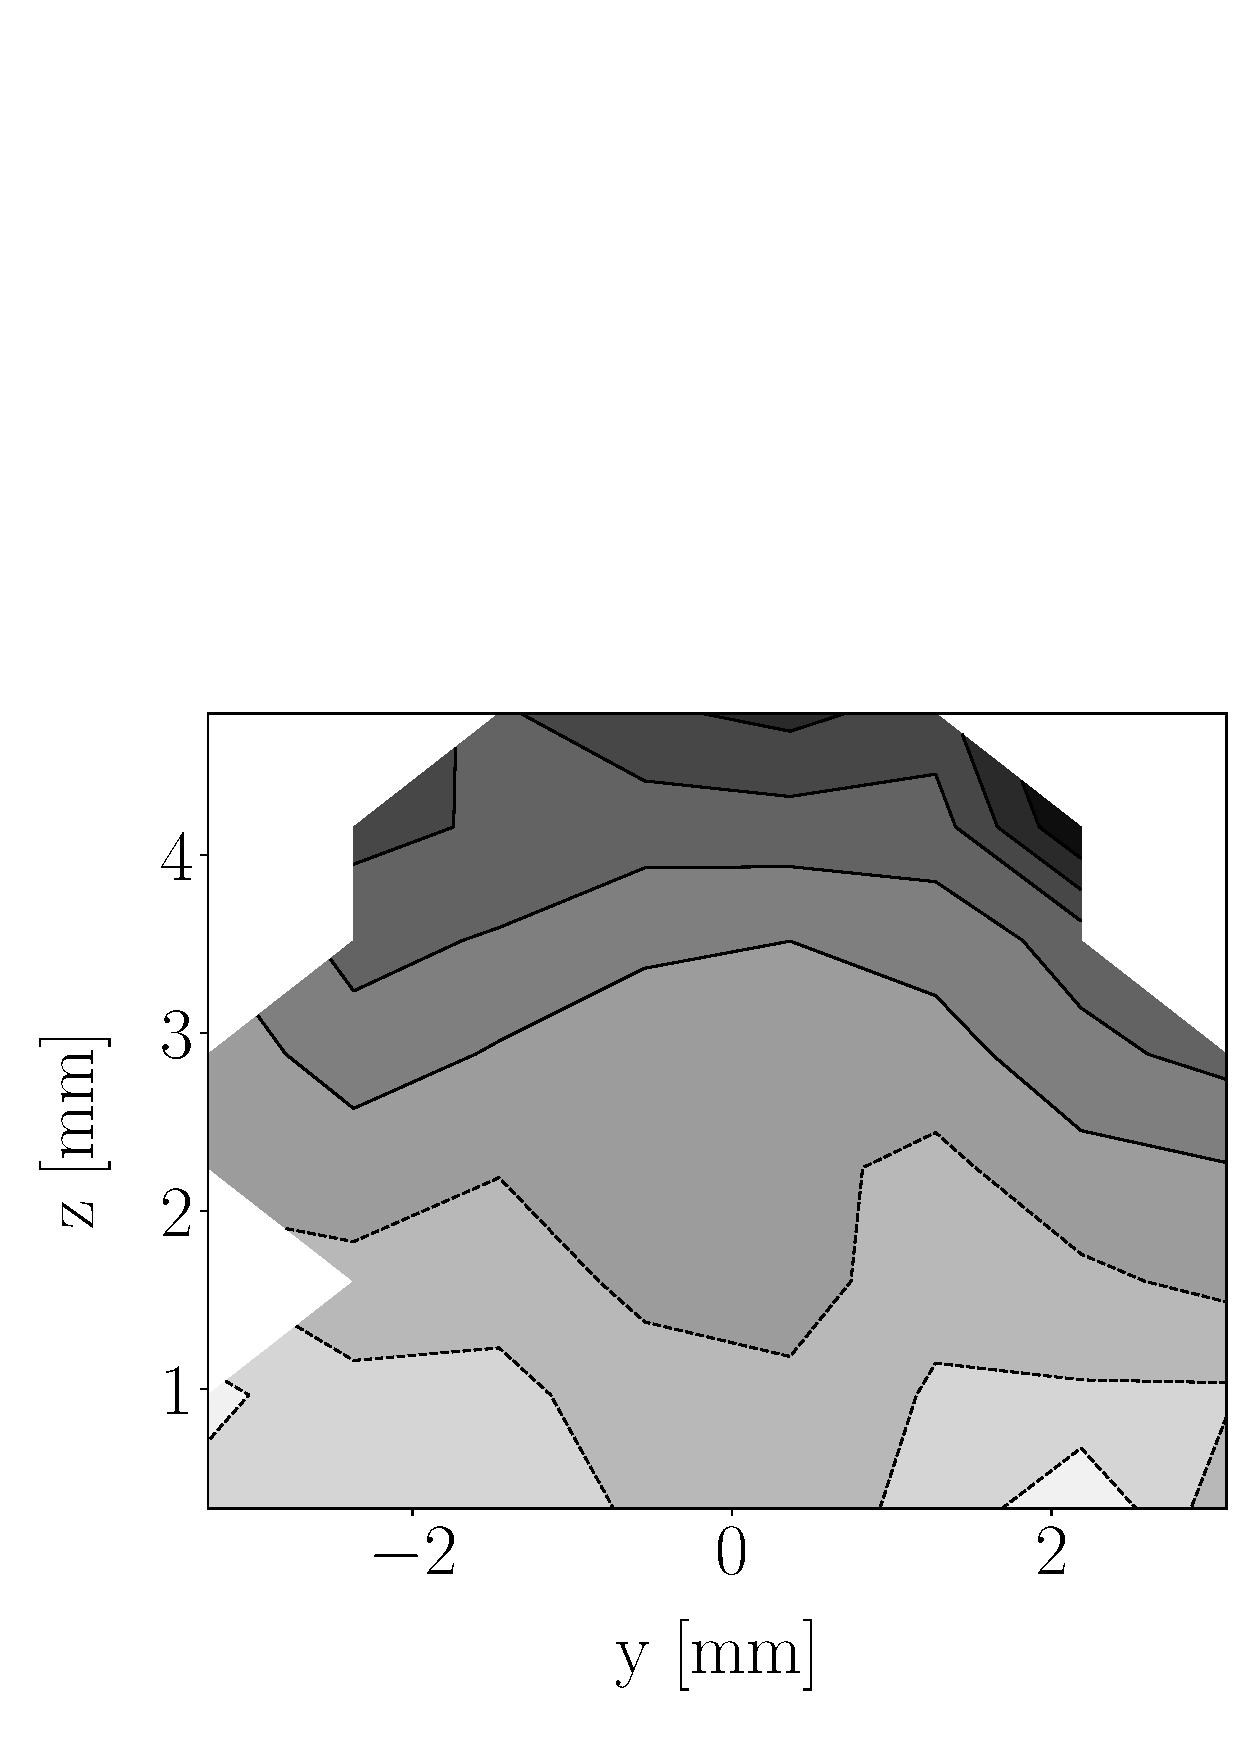
\includegraphics[scale=\scaleSLIJICF]{./part2_developments/figures_ch5_resolved_JICF/injectors_SLI/uG100_dx20_x05_uz_mean_map}
   %\caption{Case UG100\_DX10: crossflow planes}
   %\label{} 
\end{subfigure}
\caption{Spray states at x = 5 mm for case UG100\_DX20}
\label{fig:injectors_sli_uG100_dx20_x05}
\end{figure}


%%%%%%%%%%%%%%%% UG100_DX10, x = 10 mm


\begin{figure}[h!]
\centering
\begin{subfigure}[b]{0.3\textwidth}
	\centering
   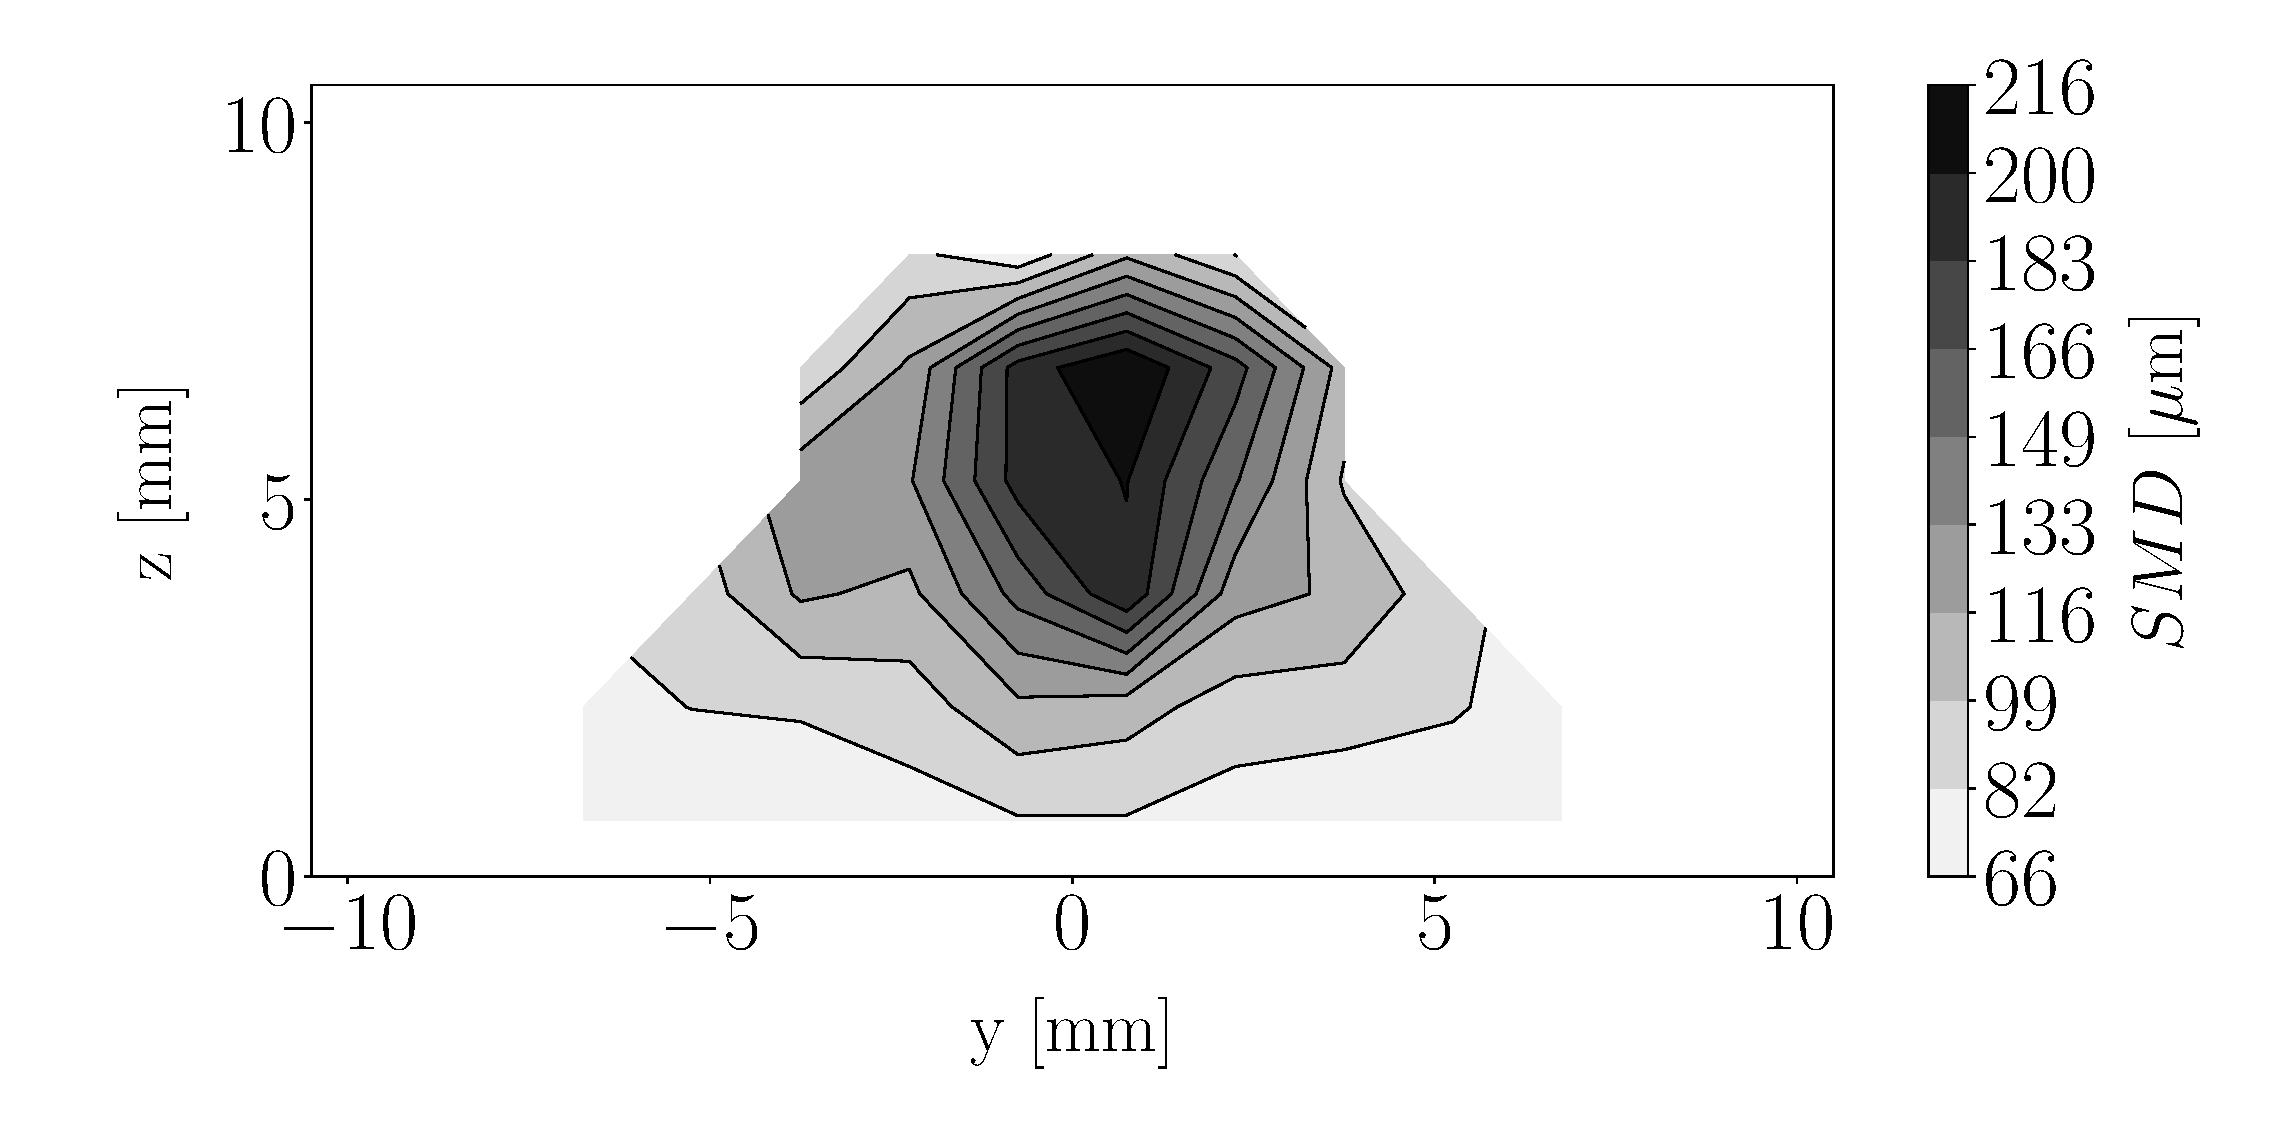
\includegraphics[scale=\scaleSLIJICF]{./part2_developments/figures_ch5_resolved_JICF/injectors_SLI/uG100_dx20_x10_SMD_map}
   %\caption{Case UG100\_DX20: crossflow planes}
   %\label{} 
\end{subfigure}
   \hspace{0.17in}
\begin{subfigure}[b]{0.3\textwidth}
	\centering
   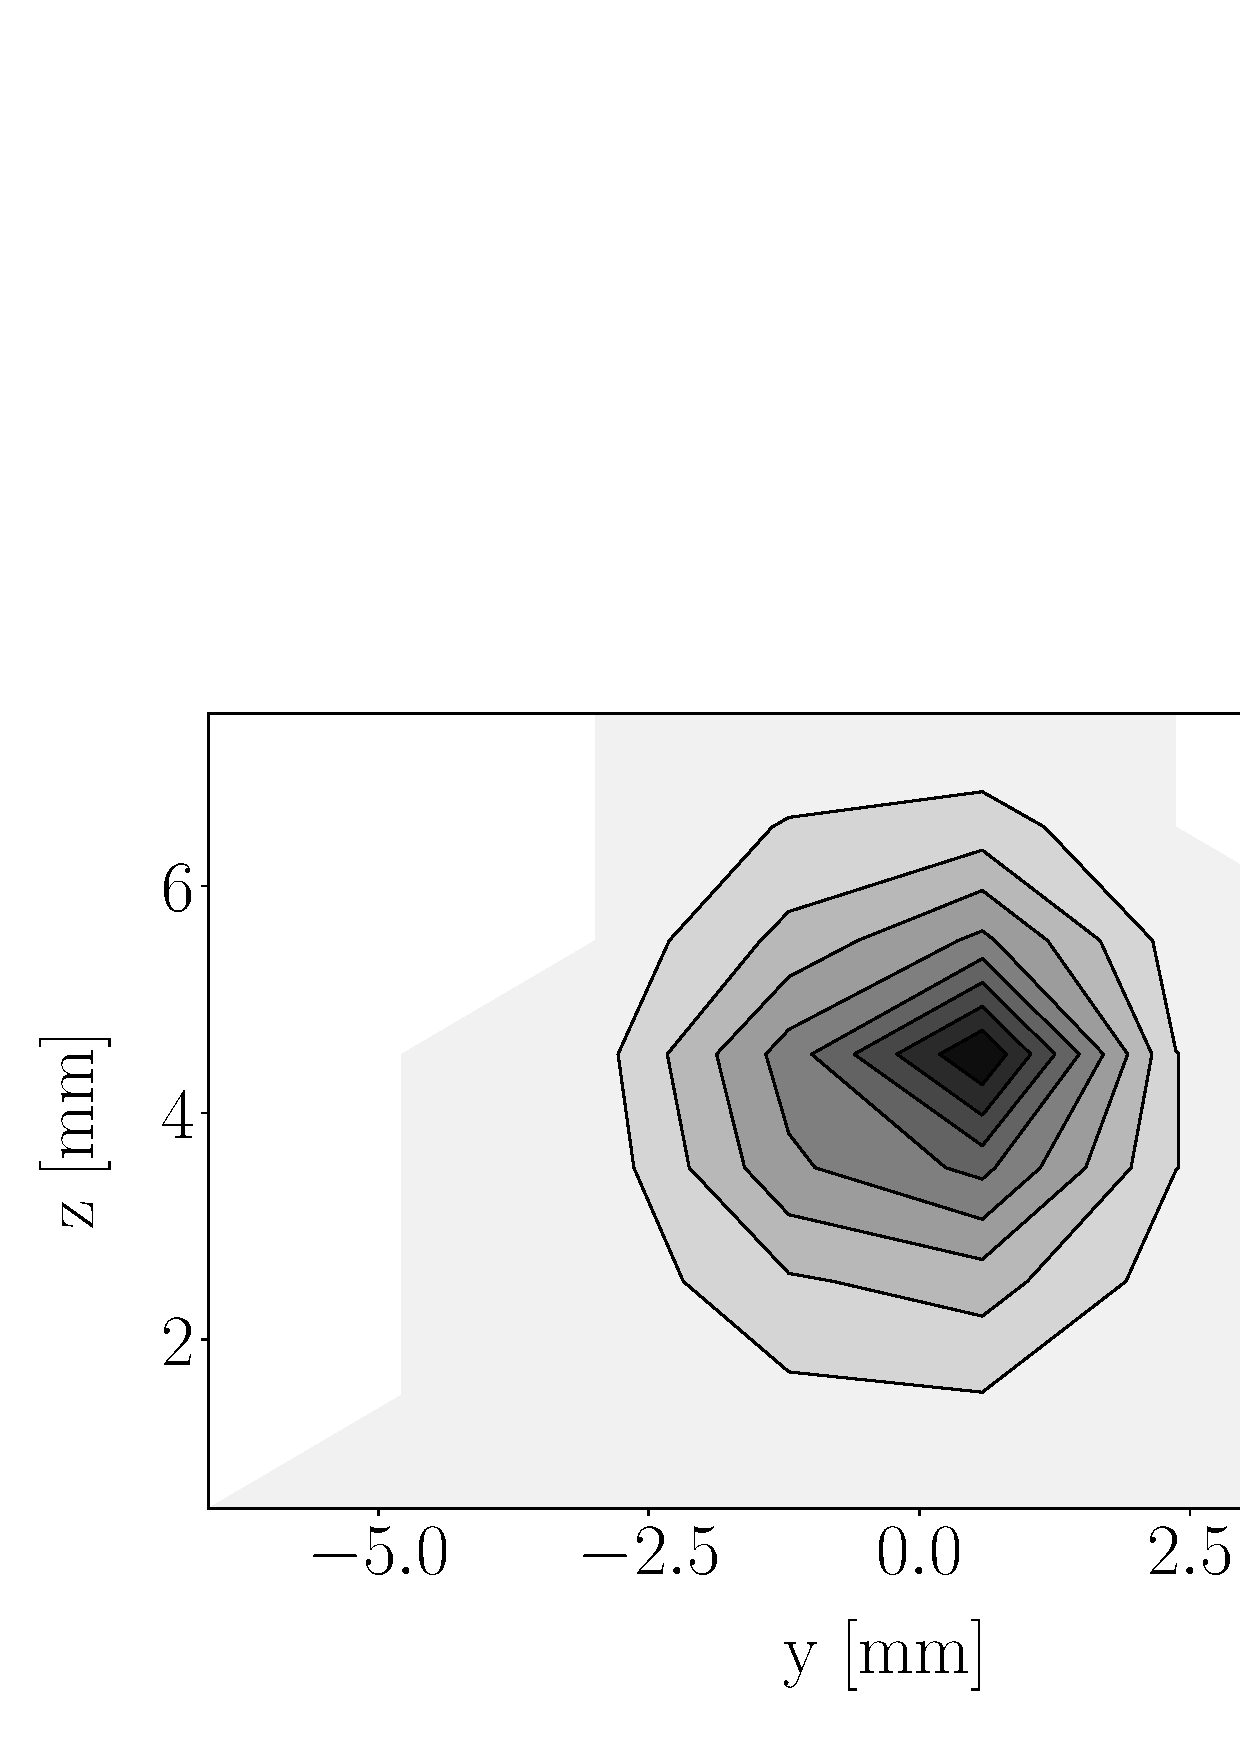
\includegraphics[scale=\scaleSLIJICF]{./part2_developments/figures_ch5_resolved_JICF/injectors_SLI/uG100_dx20_x10_volume_flux_map}
   %\caption{Case UG100\_DX20: filming planes}
   %\label{}
\end{subfigure}
   \hspace{0.17in}
\begin{subfigure}[b]{0.3\textwidth}
	\centering
   \includegraphics[scale=\scaleSLIJICF]{./part2_developments/figures_ch5_resolved_JICF/injectors_SLI/uG100_dx20_x10_convergence_map}
   %\caption{Case UG100\_DX10: crossflow planes}
   %\label{} 
\end{subfigure}

\vskip\baselineskip

\begin{subfigure}[b]{0.3\textwidth}
	\centering
   \includegraphics[scale=\scaleSLIJICF]{./part2_developments/figures_ch5_resolved_JICF/injectors_SLI/uG100_dx20_x10_ux_mean_map}
   %\caption{Case UG100\_DX20: crossflow planes}
   %\label{} 
\end{subfigure}
   \hspace{0.17in}
\begin{subfigure}[b]{0.3\textwidth}
	\centering
   \includegraphics[scale=\scaleSLIJICF]{./part2_developments/figures_ch5_resolved_JICF/injectors_SLI/uG100_dx20_x10_uy_mean_map}
   %\caption{Case UG100\_DX20: filming planes}
   %\label{}
\end{subfigure}
   \hspace{0.17in}
\begin{subfigure}[b]{0.3\textwidth}
	\centering
   \includegraphics[scale=\scaleSLIJICF]{./part2_developments/figures_ch5_resolved_JICF/injectors_SLI/uG100_dx20_x10_uz_mean_map}
   %\caption{Case UG100\_DX10: crossflow planes}
   %\label{} 
\end{subfigure}
\caption{Spray states at x = 10 mm for case UG100\_DX20}
\label{fig:injectors_sli_uG100_dx20_x10}
\end{figure}


%%%%%%%%%%%%%%%% UG100_DX10, x = 15 mm


\begin{figure}[h!]
\centering
\begin{subfigure}[b]{0.3\textwidth}
	\centering
   \includegraphics[scale=\scaleSLIJICF]{./part2_developments/figures_ch5_resolved_JICF/injectors_SLI/uG100_dx20_x15_SMD_map}
   %\caption{Case UG100\_DX20: crossflow planes}
   %\label{} 
\end{subfigure}
   \hspace{0.17in}
\begin{subfigure}[b]{0.3\textwidth}
	\centering
   \includegraphics[scale=\scaleSLIJICF]{./part2_developments/figures_ch5_resolved_JICF/injectors_SLI/uG100_dx20_x15_volume_flux_map}
   %\caption{Case UG100\_DX20: filming planes}
   %\label{}
\end{subfigure}
   \hspace{0.17in}
\begin{subfigure}[b]{0.3\textwidth}
	\centering
   \includegraphics[scale=\scaleSLIJICF]{./part2_developments/figures_ch5_resolved_JICF/injectors_SLI/uG100_dx20_x15_convergence_map}
   %\caption{Case UG100\_DX10: crossflow planes}
   %\label{} 
\end{subfigure}

\vskip\baselineskip

\begin{subfigure}[b]{0.3\textwidth}
	\centering
   \includegraphics[scale=\scaleSLIJICF]{./part2_developments/figures_ch5_resolved_JICF/injectors_SLI/uG100_dx20_x15_ux_mean_map}
   %\caption{Case UG100\_DX20: crossflow planes}
   %\label{} 
\end{subfigure}
   \hspace{0.17in}
\begin{subfigure}[b]{0.3\textwidth}
	\centering
   \includegraphics[scale=\scaleSLIJICF]{./part2_developments/figures_ch5_resolved_JICF/injectors_SLI/uG100_dx20_x15_uy_mean_map}
   %\caption{Case UG100\_DX20: filming planes}
   %\label{}
\end{subfigure}
   \hspace{0.17in}
\begin{subfigure}[b]{0.3\textwidth}
	\centering
   \includegraphics[scale=\scaleSLIJICF]{./part2_developments/figures_ch5_resolved_JICF/injectors_SLI/uG100_dx20_x15_uz_mean_map}
   %\caption{Case UG100\_DX10: crossflow planes}
   %\label{} 
\end{subfigure}
\caption{Spray states at x = 15 mm for case UG100\_DX20}
\label{fig:injectors_sli_uG100_dx20_x15}
\end{figure}

%\subsection{Feeding the models (??)}
%Find a more attractive name


\clearpage

\subsubsection*{Case UG100\_DX20\_NT}



%%%%%%%%%%%%%%%% UG100_DX20_NT, x = 5 mm


\begin{figure}[h!]
\centering
\begin{subfigure}[b]{0.3\textwidth}
	\centering
   \includegraphics[scale=\scaleSLIJICF]{./part2_developments/figures_ch5_resolved_JICF/injectors_SLI/uG100_dx20_x05_NT_SMD_map}
   %\caption{Case UG100\_DX20: crossflow planes}
   %\label{} 
\end{subfigure}
   \hspace{0.17in}
\begin{subfigure}[b]{0.3\textwidth}
	\centering
   \includegraphics[scale=\scaleSLIJICF]{./part2_developments/figures_ch5_resolved_JICF/injectors_SLI/uG100_dx20_x05_NT_volume_flux_map}
   %\caption{Case UG100\_DX20: filming planes}
   %\label{}
\end{subfigure}
   \hspace{0.17in}
\begin{subfigure}[b]{0.3\textwidth}
	\centering
   \includegraphics[scale=\scaleSLIJICF]{./part2_developments/figures_ch5_resolved_JICF/injectors_SLI/uG100_dx20_x05_NT_convergence_map}
   %\caption{Case UG100\_DX10: crossflow planes}
   %\label{} 
\end{subfigure}

\vskip\baselineskip

\begin{subfigure}[b]{0.3\textwidth}
	\centering
   \includegraphics[scale=\scaleSLIJICF]{./part2_developments/figures_ch5_resolved_JICF/injectors_SLI/uG100_dx20_x05_NT_ux_mean_map}
   %\caption{Case UG100\_DX20: crossflow planes}
   %\label{} 
\end{subfigure}
   \hspace{0.17in}
\begin{subfigure}[b]{0.3\textwidth}
	\centering
   \includegraphics[scale=\scaleSLIJICF]{./part2_developments/figures_ch5_resolved_JICF/injectors_SLI/uG100_dx20_x05_NT_uy_mean_map}
   %\caption{Case UG100\_DX20: filming planes}
   %\label{}
\end{subfigure}
   \hspace{0.17in}
\begin{subfigure}[b]{0.3\textwidth}
	\centering
   \includegraphics[scale=\scaleSLIJICF]{./part2_developments/figures_ch5_resolved_JICF/injectors_SLI/uG100_dx20_x05_NT_uz_mean_map}
   %\caption{Case UG100\_DX10: crossflow planes}
   %\label{} 
\end{subfigure}
\caption{Spray states at x = 5 mm for case UG100\_DX20\_NT}
\label{fig:injectors_sli_uG100_dx20_x05_NT}
\end{figure}


%%%%%%%%%%%%%%%% UG100_DX20_NT, x = 10 mm

\begin{figure}[h!]
\centering
\begin{subfigure}[b]{0.3\textwidth}
	\centering
   \includegraphics[scale=\scaleSLIJICF]{./part2_developments/figures_ch5_resolved_JICF/injectors_SLI/uG100_dx20_x10_NT_SMD_map}
   %\caption{Case UG100\_DX20: crossflow planes}
   %\label{} 
\end{subfigure}
   \hspace{0.17in}
\begin{subfigure}[b]{0.3\textwidth}
	\centering
   \includegraphics[scale=\scaleSLIJICF]{./part2_developments/figures_ch5_resolved_JICF/injectors_SLI/uG100_dx20_x10_NT_volume_flux_map}
   %\caption{Case UG100\_DX20: filming planes}
   %\label{}
\end{subfigure}
   \hspace{0.17in}
\begin{subfigure}[b]{0.3\textwidth}
	\centering
   \includegraphics[scale=\scaleSLIJICF]{./part2_developments/figures_ch5_resolved_JICF/injectors_SLI/uG100_dx20_x10_NT_convergence_map}
   %\caption{Case UG100\_DX10: crossflow planes}
   %\label{} 
\end{subfigure}

\vskip\baselineskip

\begin{subfigure}[b]{0.3\textwidth}
	\centering
   \includegraphics[scale=\scaleSLIJICF]{./part2_developments/figures_ch5_resolved_JICF/injectors_SLI/uG100_dx20_x10_NT_ux_mean_map}
   %\caption{Case UG100\_DX20: crossflow planes}
   %\label{} 
\end{subfigure}
   \hspace{0.17in}
\begin{subfigure}[b]{0.3\textwidth}
	\centering
   \includegraphics[scale=\scaleSLIJICF]{./part2_developments/figures_ch5_resolved_JICF/injectors_SLI/uG100_dx20_x10_NT_uy_mean_map}
   %\caption{Case UG100\_DX20: filming planes}
   %\label{}
\end{subfigure}
   \hspace{0.17in}
\begin{subfigure}[b]{0.3\textwidth}
	\centering
   \includegraphics[scale=\scaleSLIJICF]{./part2_developments/figures_ch5_resolved_JICF/injectors_SLI/uG100_dx20_x10_NT_uz_mean_map}
   %\caption{Case UG100\_DX10: crossflow planes}
   %\label{} 
\end{subfigure}
\caption{Spray states at x = 10 mm for case UG100\_DX20\_NT}
\label{fig:injectors_sli_uG100_dx20_x10_NT}
\end{figure}


\clearpage



\subsection{Inhomogeneity of sprays}
\label{subsec:SPS_inhomogeneity_sprays}

The resulting spray from a JICF is highly polydisperse and velocity-inhomogeneous, as shown by the spatial distribution of SMD and mean velocities in the previous maps. The proposed SLI approach allows to account in a direct manner of this polydisperse and inhomogeneous nature of the spray when prescribing spatially discretized statistics in dispersed-phase simulations. This spatial discretization procedure can also be seen as dividing the global in-plane accumulated spray into several individual sprays, each one of them contained in every discretization probe. Each of these sprays then can be represented as a monodisperse spray by accounting only for mean statistics on the diameters and velocities, such as the SMD and mean velocities. However, the polydispersity and inhomogeneity of each probe's spray should also be taken into account when performing injection.

In order to illustrate this inhomogeneity within the local probes, Figure \ref{fig:injectors_SLI_extra_UG100_DX10_x05} shows the maps of volume flux, arithmetic mean and volume-weighted velocities at $x = 5$ mm for case UG100\_DX10. The discretization grid is shown, and the probe containing the spray with the largest flux (i.e. with more droplets) is highlighted in blue. The velocity maps show a different spatial distribution of the velocity when considering volume-weighted or not: the VW velocity displays lower values in all the plane, since actually more importance is given to the large droplets which have less velocity than the smaller ones due to a lower relaxation time towards the gaseous phase. Exceptions are seen in the regions with the lowest volume fluxes, since in those the amount of droplets is scarce and the mean and volume-weighted velocities are closer (and identical in probes containing sprays with only one sampled droplet). The spray at the probe containing the maximum flux is analyzed by plotting the histograms of droplet size $D$ and axial velocity $u$ as well as the scatterplot $D - u$ in Figure \ref{fig:injectors_SLI_extra_UG100_DX10_x05}. In the size histogram the SMD is highlighted: if only the SMD is injected in the dispersed-phase simulations, a wide range of droplets sizes is actually neglected when prescribing the spray. Injection of a spray size distribution $f_0$ better representing the spray histogram will solvent this issue. The velocity histogram shows also a wide range of droplets velocities with respect to the mean ones: injecting a stochastic velocity given by a law such as the one from Eq. (\ref{eq:ch4_lagrangian_injection_velocity_with_mean_and_rms}), which also accounts for the RMS component will then consider the inhomogeneity of the droplets velocities. It is also noticeable the difference between arithmetic mean and VW velocities, 52 against 44 $m s^{-1}$ respectively: such differences at injection could greatly impact secondary atomization of droplets, which is highly dependent on the $We$ based on the relative velocity. These two influences, i.e polydispersity through $f_0$ and variations in injection velocity through Eq. (\ref{eq:ch4_lagrangian_injection_velocity_with_mean_and_rms}), will be investigated in the next chapter. What is still missing is, however, a prescription of the velocities based on both $f_0$ and inhomogeneous velocity where the actual injection velocity is conditioned to its size. The scatterplot $D-u$ at Figure \ref{fig:injectors_SLI_extra_UG100_DX10_x05} right. The arithmetic mean and VW velocities are represented by the horizontal black lines, while the $SMD$ is given by the vertical green line. The points where curves cross would represent the injection velocity and diameters if a monodisperse spray were to be injected: considering also the RMS through Eq. (\ref{eq:ch4_lagrangian_injection_velocity_with_mean_and_rms}) would enlarge the range of velocities to be injected, while also including a $f_0$ would enlarge the range of droplets sizes injected. The red line would represent the approach where the droplets velocities are prescribed according to their size: this strategy is called sectional approach, and has been succesfully tested in lagrangian sprays \citepColor[vie_accounting_2013]. Such technique has not been implemented in this work, but is considered as an interesting perspective for the future of SLI.


\begin{figure}[h!]
\centering
\begin{subfigure}[b]{0.3\textwidth}
	\centering
   \includegraphics[scale=0.225]{./part2_developments/figures_ch5_resolved_JICF/injectors_SLI_extra/uG100_dx10_x05_volume_flux_map}
   %\caption{Case UG100\_DX20: crossflow planes}
   %\label{} 
\end{subfigure}
   \hspace{0.17in}
\begin{subfigure}[b]{0.3\textwidth}
	\centering
   \includegraphics[scale=0.225]{./part2_developments/figures_ch5_resolved_JICF/injectors_SLI_extra/uG100_dx10_x05_ux_mean_map}
   %\caption{Case UG100\_DX20: filming planes}
   %\label{}
\end{subfigure}
   \hspace{0.17in}
\begin{subfigure}[b]{0.3\textwidth}
	\centering
   \includegraphics[scale=0.225]{./part2_developments/figures_ch5_resolved_JICF/injectors_SLI_extra/uG100_dx10_x05_ux_mean_VW_map}
   %\caption{Case UG100\_DX10: crossflow planes}
   %\label{} 
\end{subfigure}

\caption{Volume flux, arithmetic mean and volume-weighted axial velocities at $x = 5$ mm from case UG100\_DX10}
\label{fig:injectors_SLI_extra_UG100_DX10_x05}
\end{figure}

\clearpage


\begin{figure}[h!]
\centering
\begin{subfigure}[b]{0.3\textwidth}
	\centering
   \includegraphics[scale=0.24]{./part2_developments/figures_ch5_resolved_JICF/injectors_SLI_extra/uG100_dx10_x05_size_histogram}
   %\caption{Case UG100\_DX20: crossflow planes}
   %\label{} 
\end{subfigure}
   \hspace{0.17in}
\begin{subfigure}[b]{0.3\textwidth}
	\centering
   \includegraphics[scale=0.24]{./part2_developments/figures_ch5_resolved_JICF/injectors_SLI_extra/uG100_dx10_x05_vel_histogram}
   %\caption{Case UG100\_DX20: filming planes}
   %\label{}
\end{subfigure}
   \hspace{0.17in}
\begin{subfigure}[b]{0.3\textwidth}
	\centering
   \includegraphics[scale=0.24]{./part2_developments/figures_ch5_resolved_JICF/injectors_SLI_extra/uG100_dx10_x05_vel_scatter}
   %\caption{Case UG100\_DX10: crossflow planes}
   %\label{} 
\end{subfigure}

\caption[Histograms of droplets diameters $D$ (\textsl{left}) and axial velocity $u$ (\textsl{center}), and scatterplot $D - u$ (\textsl{right})]{Histograms of droplets diameters $D$ (\textsl{left}) and axial velocity $u$ (\textsl{center}), and scatterplot $D - u$ (\textsl{right}) for the spray contained within the highlighted probe of Figure \ref{fig:injectors_SLI_extra_UG100_DX10_x05}}
\label{fig:injectors_extra_velocities_interesting}
\end{figure}



